%Version 3.1 December 2024
\documentclass[pdflatex,sn-mathphys-num,referee,lineno]{sn-jnl}

\usepackage{graphicx}%
\usepackage{xr}%
\externaldocument{../supplementary/supplementary_material}%
\usepackage{multirow}%
\usepackage{amsmath,amssymb,amsfonts}%
\usepackage{amsthm}%
\usepackage{mathrsfs}%
\usepackage[title]{appendix}%
\usepackage{xcolor}%
\usepackage{textcomp}%
\usepackage{manyfoot}%
\usepackage{booktabs}%
\usepackage{algorithm}%
\usepackage{algorithmicx}%
\usepackage{algpseudocode}%
\usepackage{listings}%
\usepackage{pdflscape}% For landscape pages
\usepackage{rotating}%
\graphicspath{{../figures/}}

\theoremstyle{thmstyleone}%
\newtheorem{theorem}{Theorem}%
\newtheorem{proposition}[theorem]{Proposition}%

\theoremstyle{thmstyletwo}%
\newtheorem{example}{Example}%
\newtheorem{remark}{Remark}%

\theoremstyle{thmstylethree}%
\newtheorem{definition}{Definition}%

\raggedbottom

\begin{document}

\title[C1Q/SPP1 Macrophage Spatial Context]{C1Q/SPP1 Macrophage Spatial Context as a Cross-Dataset Traceability Feature in Non-Small Cell Lung Cancer: A Public Multi-Cohort Cancer-Informatics Evidence Synthesis}

\author*[1]{\fnm{Anonymous} \sur{Author}}

\affil*[1]{\orgname{Anonymous Institution}, \orgaddress{\country{Anonymous}}}

\abstract{\textbf{Objectives:} Public cancer-informatics resources provide an opportunity to test whether macrophage-associated complement programs are traceable features of non-small cell lung cancer (NSCLC) tumor-microenvironment context. However, retrospective multi-omics analyses are vulnerable to overinterpretation when prognostic, spatial, and immunotherapy-response signals are presented as clinical tools or mechanistic proof.

    \textbf{Methods:} We performed a conservative public-data evidence synthesis centered on the C1Q/SPP1 macrophage axis. Bulk transcriptomic and clinical data from TCGA NSCLC were used for discovery and score-behavior assessment after quality control. External prognostic traceability was evaluated in GSE31210 patients with complete follow-up. Two small NSCLC immune-checkpoint-blockade (ICB) cohorts and one melanoma exploratory ICB cohort were analyzed separately as response-association datasets. Spatial context was assessed using 10x Visium sections and Nanostring CosMx SMI data, with inference emphasized at the patient, section, or sample-contrast level rather than at the spot or single-cell count level. Mendelian-randomization analyses were used for gene prioritization, not as definitive causal or therapeutic evidence.

    \textbf{Results:} Nested cross-validation identified a stable 95-feature set enriched for immune and macrophage-context signals. C1QA, C1QB, and C1QC showed section-level spatial autocorrelation in patient-limited spatial datasets (Moran's I approximately 0.35--0.39), whereas SPP1 showed stronger spatial clustering (Moran's I = 0.712), consistent with a distinct macrophage-associated compartmentalized context. Retrospective model benchmarking showed statistically detectable but modest prognostic discrimination in TCGA and attenuated external performance in GSE31210; therefore, the model is reported as exploratory score behavior rather than as a clinical prediction tool. The ICB cohorts showed directional response associations, but sample size and tumor-type heterogeneity preclude clinical claims.

    \textbf{Conclusions:} C1Q/SPP1 captures a cross-dataset macrophage-spatial context in public NSCLC resources and may serve as a traceability feature for immune-active versus macrophage-compartmentalized tumor-microenvironment states. The findings are hypothesis-generating and require prospective, spatially resolved, and experimental validation before clinical implementation or therapeutic targeting can be considered.}

\keywords{Non-small cell lung cancer, Cancer informatics, C1Q, SPP1, macrophage context, spatial transcriptomics, reproducibility, traceability feature}

\maketitle

\section{Introduction}\label{sec:intro}

Non-small cell lung cancer (NSCLC) remains a major cause of cancer mortality, and immune checkpoint blockade has improved outcomes for a subset of patients \cite{sungGlobalCancerStatistics2021b, chenNonsmallcellLungCancers2014, reckPembrolizumabChemotherapyPDL1positive2016, herbstAtezolizumabFirstlineTreatment2020, gandhiPembrolizumabChemotherapyMetastatic2018}. However, PD-L1 expression, tumor mutational burden, and bulk immune-expression summaries do not fully capture the spatial and cellular organization of the tumor microenvironment (TME) \cite{marabelleAssociationTumourMutational2020, topalianMechanismdrivenBiomarkersGuide2016}. Spatial transcriptomics and single-cell technologies now make it possible to examine whether immune programs visible in bulk data also map to spatial contexts that can be traced across available datasets \cite{stahlVisualizationAnalysisGene2016, marxMethodYearSpatially2021, zilionisSinglecellTranscriptomicsHuman2019}.

C1q, encoded by \textit{C1QA}, \textit{C1QB}, and \textit{C1QC}, is produced largely by macrophage and dendritic-cell lineages in the TME. Prior work suggests that complement-associated macrophage states may accompany either immune activation or tumor-promoting inflammation, depending on context. \textit{SPP1}-positive macrophage programs, by contrast, are often linked to stromal remodeling and immune exclusion. These observations motivate a narrower and more testable question: can the C1Q/SPP1 macrophage axis be traced across public NSCLC transcriptomic, spatial, and clinical resources without overstating clinical or mechanistic certainty?

The present study is intentionally framed as a public cancer-informatics evidence synthesis. We do not claim to establish a clinical diagnostic assay, a treatment-selection tool, or a definitive mechanism. Instead, we evaluate whether C1Q/SPP1 behaves as a traceability feature linking macrophage context, spatial organization, retrospective survival associations, and exploratory immunotherapy-response signals. This conservative framing separates data-supported observations from hypotheses that require prospective and experimental validation.

\section{Methods}\label{sec:methods}

\subsection{Study Design and Evidence Hierarchy}\label{subsec:study_design}

This study used a staged, retrospective public-data design \cite{subramanianMultiomicsDataIntegration2020, chaudharyDeepLearningBased2018, sammutMultiomicMachineLearning2022}. The evidence hierarchy was defined before interpretation: (1) TCGA NSCLC was used for discovery and internal score-behavior assessment; (2) GEO cohorts were used for external prognostic traceability where complete follow-up was available; (3) Visium and CosMx SMI datasets were used to evaluate spatial context, with inference emphasized at the patient, section, or paired-contrast level; and (4) immunotherapy-treated cohorts were treated as exploratory response-association datasets because of small sample sizes and tumor-type heterogeneity (Figure \ref{fig:1}).

\subsubsection{Data Acquisition and Quality Control}

\textbf{Discovery Cohort (TCGA):} TCGA LUAD and LUSC transcriptomic and clinical data were retrieved from the NCI Genomic Data Commons \cite{hoadleyCelloforiginPatternsDominate2018a, thecancergenomeatlasresearchnetworkComprehensiveMolecularProfiling2014a}. A total of 1,100 TCGA NSCLC tumor samples were initially considered (595 LUAD and 505 LUSC). After quality control and availability filtering, 1,038 samples contributed to discovery analyses. Analyses requiring complete survival, stage, or model features used the corresponding complete-case subsets; denominators are reported with each analysis.

\textbf{Spatial Transcriptomics Data:} For spatially resolved context analysis, we incorporated 10x Genomics Visium and Nanostring CosMx SMI datasets. Quality control, normalization, and platform-specific processing are described in the Supplementary Methods and source-data manifest. Spatial inference was deliberately anchored to patient, section, or sample-contrast units; spots and cells were treated as measurement units within those samples rather than as independent biological replicates.
\begin{itemize}
    \item \textbf{10x Visium:} Included 8 tissue sections from 1 patient (Supplementary Table S12), utilizing a 55 $\mu$m spot diameter for tissue-level spatial mapping.
    \item \textbf{CosMx SMI:} Encompassed 8 tissue sections from 5 NSCLC patients, containing approximately 800,000 profiled cells targeted with a 960-gene RNA panel. Cell counts were treated as descriptive observations; independent inference was anchored to samples, sections, and paired contrasts.
\end{itemize}

\textbf{External Cohorts:} Clinical and expression data were retrieved from GEO. GSE31210 contained 226 lung adenocarcinoma samples after exclusion of non-tumor controls and 178 patients with complete follow-up for survival analysis. GSE126044 and GSE135222 were treated as small NSCLC ICB response-association cohorts, whereas GSE91061 was treated as a melanoma exploratory cohort only. These datasets were not pooled as confirmatory NSCLC immunotherapy validation.

\subsection{C1Q/SPP1 Traceability Framework}\label{subsec:framework}

We implemented a multi-stage traceability framework to evaluate whether C1Q/SPP1 macrophage context is traceable across data layers:

\textbf{Phase 1: MR-based gene prioritization:} Mendelian randomization (MR) was used to prioritize genes with expression-linked immune-context associations \cite{daveysmithMendelianRandomizationCan2003}, not to prove mechanism or treatment relevance. We used eQTL data from eQTLGen \cite{vosaLargescaleCisTranseQTL2021} and GTEx v8 with TwoSampleMR (v0.5.6), and inspected sensitivity diagnostics before assigning confidence.

\textbf{Phase 2: Retrospective score-behavior assessment:} Machine-learning algorithms were benchmarked to assess whether the stable feature set carried survival-associated signal. The resulting models were not interpreted as clinical tools and no fixed clinical cutoff is proposed.

\textbf{Phase 3: Spatial context characterization:} A C1Q/SPP1-centered scoring approach was used to evaluate macrophage-associated spatial organization and CD8-marker context in Visium and CosMx data.

\begin{table*}[htbp]
    \caption{Claim-evidence-boundary framework used for interpretation}\label{tab:evidence_boundary}
    \small
    \begin{tabular*}{\textwidth}{@{\extracolsep\fill}p{0.18\textwidth}p{0.22\textwidth}p{0.24\textwidth}p{0.20\textwidth}}
        \toprule
        Claim domain & Evidence layer & Supported interpretation & Boundary \\
        \midrule
        C1Q/SPP1 macrophage context & TCGA/GEO transcriptomics, feature stability, immune-context correlations & The axis is traceable across public expression datasets as a macrophage-context feature & Not a diagnostic assay or tumor-specific marker \\
        Spatial organization & Visium sections from one patient and CosMx sections from five NSCLC patients & C1Q and SPP1 show non-random spatial patterns in the available sections & Spots/cells are measurement units, not independent biological replicates; patient-level validation remains limited \\
        MR-based prioritization & eQTL-based two-sample MR with sensitivity diagnostics & MR highlights candidates for follow-up under instrumental-variable assumptions & Not causal proof, target validation, or evidence of therapeutic actionability \\
        Retrospective outcome score & TCGA internal assessment and GSE31210 traceability & The feature set carries modest outcome-linked signal and can be used descriptively & No locked clinical cutoff, no prospective validation, and no treatment-selection claim \\
        ICB response association & Two small NSCLC ICB cohorts and one melanoma exploratory cohort & Directional response-associated separation is observed in small cohorts & Not NSCLC ICB validation and not evidence of superiority over PD-L1, TMB, or clinical baselines \\
        \botrule
    \end{tabular*}
    \footnotetext{This table defines the interpretive boundaries used throughout the manuscript and the public evidence-chain map.}
\end{table*}

\subsection{Neighborhood Enrichment Analysis}\label{subsec:neighborhood}

Neighborhood enrichment analysis was performed in CosMx SMI data to describe local co-occurrence between C1Q-associated macrophage states and CD8-marker-positive contexts. A 50 $\mu$m radius was used around each index cell, and observed neighborhood composition was compared with a permutation-based null distribution (N=1,000 permutations). Because the number of independent patients was limited, these results were interpreted as local spatial-context support rather than definitive evidence of cell-cell signaling or causal recruitment.

\subsection{Data Preprocessing and Statistical Analysis}\label{subsec:preprocessing}

\subsubsection{Transcriptome Data Preprocessing}

Bulk transcriptomic datasets were processed using dataset-appropriate normalization. TCGA RNA-seq expression values were filtered for low expression, log-transformed where appropriate, and aligned by gene symbol. External microarray data were quantile normalized or used as normalized series-matrix data when provided by GEO. Cross-platform analyses used within-cohort z-score scaling after feature alignment; platform-specific effects were not interpreted biologically. Excluded samples and feature-retention decisions are documented in the source-data manifest.

\subsubsection{Statistical Analysis}

All statistical analyses were performed using R and Python. Python-based data manipulation and visualization used Pandas \cite{mckinneyDataStructuresStatistical2010a}, NumPy \cite{harrisArrayProgrammingNumPy2020}, SciPy \cite{virtanenSciPy10Fundamental2020}, Matplotlib \cite{hunterMatplotlib2DGraphics2007}, and Seaborn \cite{waskomSeabornStatisticalData2021}. Machine-learning tasks used Scikit-learn \cite{pedregosaScikitlearnMachineLearning2011a}. Survival analysis used Kaplan--Meier curves and Cox proportional hazards models. Model performance was evaluated with time-dependent AUC, concordance index (C-index), and hazard ratios with 95\% confidence intervals where available. Data and code availability are detailed in the Declarations section.

\subsection{Sample Size and Statistical Power}\label{subsec:power}

The TCGA discovery cohort (N=1,038 after quality control) was adequate for exploratory feature discovery and internal score-behavior assessment. External cohorts were smaller and had lower event counts; therefore, external survival and immunotherapy-response results were interpreted as traceability or exploratory association rather than confirmatory validation. No prospective sample-size calculation was possible because the study used public retrospective data.

\subsection{Nested Cross-Validation Framework}\label{sec:nested_cv}

To reduce data leakage and estimate feature stability, we implemented a 5$\times$5 nested cross-validation framework.

\textbf{Outer Loop (Model Evaluation):}
\begin{itemize}
    \item 5-fold stratified cross-validation (StratifiedKFold)
    \item Stratification basis: Vital status (alive/dead)
    \item Each fold: Training set 880 cases (80\%), Test set 220 cases (20\%)
    \item Random seed: 42 (ensuring reproducibility)
\end{itemize}

\textbf{Inner Loop (Feature Selection):}
\begin{itemize}
    \item 5-fold cross-validation within each outer training set
    \item LASSO-based feature selection with $\alpha$ optimization using 5-fold cross-validation and 10-fold grid search ($\alpha$ range: $10^{-5}$ to $10^{-1}$, step size: 0.01). Optimal alpha was selected based on minimum cross-validation error, with final $\lambda = 0.002$ yielding 91 non-zero coefficients (Supplementary Table S2).
    \item Features selected in 100\% of outer folds (frequency = 5/5) retained as ``core features''
\end{itemize}

This double-layer strategy separated feature selection from held-out fold assessment within TCGA. It does not replace independent prospective validation.

\subsection{Mendelian Randomization for Gene Prioritization}

We used two-sample Mendelian randomization \cite{hemaniMRbasePlatformSupports2018b} (MR), implemented in the \textit{TwoSampleMR} R package, as a gene-prioritization layer. MR estimates were interpreted as expression-linked associations under instrumental-variable assumptions, not as proof of spatial mechanism, therapeutic actionability, or clinical utility.

\textbf{Instrumental Variable Selection}
\begin{itemize}
    \item Genome-wide significance threshold: $P < 5 \times 10^{-8}$
    \item Linkage disequilibrium (LD) pruning: $r^2 < 0.001$, window size = 10,000 kb
    \item F-statistics calculated for all IVs, with $F > 10$ indicating strong instruments
\end{itemize}

\textbf{MR Methods}
\begin{itemize}
    \item \textbf{Inverse Variance Weighted (IVW)}: Primary summary estimate under standard MR assumptions.
    \item \textbf{MR-Egger}: Used to assess directional pleiotropy and provide a sensitivity estimate under weaker assumptions.
    \item \textbf{Weighted Median}: Used as a sensitivity estimate when a subset of instruments may be invalid.
\end{itemize}

\textbf{Comprehensive Sensitivity Analyses}:
\begin{enumerate}
    \item \textbf{Instrument strength}: F-statistics (median $F = 52,096.3$, 100\% strong IVs with $F > 10$)
    \item \textbf{Horizontal pleiotropy}: MR-Egger intercept test (18.5\% of genes showed no pleiotropy, $P > 0.050$)
    \item \textbf{Heterogeneity}: Cochran's Q test (62.3\% showed no significant heterogeneity, $P > 0.050$)
    \item \textbf{Outlier detection}: MR-PRESSO identified and removed outlier variants (70.0\% of genes had no outliers, $P > 0.050$)
    \item \textbf{Leave-one-out analysis}: Iteratively excluded each SNP to assess single-variant influence.
\end{enumerate}

\textbf{Exposure and Outcome Definitions}: In all MR analyses, the exposure was defined as eQTL-mediated gene-expression proxies from available summary-statistic resources. Outcomes were immune-context phenotypes or immune-infiltration proxies derived from lung-cancer resources where available. These outcomes should not be interpreted as directly measured single-cell densities or spatial phenotypes.

Detailed MR diagnostic parameters and leave-one-out sensitivity plots are provided in Supplementary Table S11 and Supplementary Figures S9--S10. Very small MR P-values were interpreted as ranking evidence within the analytic pipeline rather than as proportional evidence of effect certainty. Candidates with pleiotropy, heterogeneity, weak instruments, limited colocalization support, or bidirectional signals were interpreted cautiously.

\subsection{Spatial Transcriptomics Analysis}\label{subsec:spatial_methods}

Spatial analyses were designed to test whether C1Q/SPP1-associated expression showed non-random local structure in the available tissue sections. Because the spatial datasets contained few independent patients, all spatial statistics were interpreted as descriptive spatial-context summaries.

\subsubsection{Spatial Autocorrelation Analysis}
We quantified spatial clustering of gene expression using Moran's I statistic implemented in the 'spdep' R package, a measure of spatial autocorrelation ranging from -1 (dispersion) to +1 (clustering). We calculated Moran's I values for candidate genes across spatial locations using a queen contiguity matrix with 10,000 permutations. Genes with Moran's I $>$ 0.35 and corrected $P < 0.001$ were described as spatially clustered. The term ``hotspot'' is used descriptively and does not imply causal organization.

\subsubsection{Cell Type Deconvolution}
Cell-type context in Visium data was estimated using the GigaTIME framework and cross-checked against canonical marker expression, including CD68 for macrophage context and CD8A/CD8B for CD8-marker context. These outputs were used as contextual estimates rather than direct ground-truth cell counts. CosMx SMI was used to inspect single-cell-resolution expression and neighborhood patterns in the available sections.

\subsubsection{Spatial Co-localization Analysis}
To assess spatial context among C1Q, SPP1, and immune-marker programs, we calculated correlations and local spatial statistics across multiple spatial scales (50$\mu$m, 100$\mu$m, and 200$\mu$m where available) \cite{raviSpatiallyResolvedMultiomics2022, liSpatialTranscriptomicsTumor2022}. Bivariate Moran's I, Geary's C, and local indicators of spatial association were used as descriptive spatial summaries with permutation-based significance testing and Benjamini--Hochberg correction. These analyses were interpreted as evidence of co-localization or spatial separation, not as proof of direct biological interaction.

\subsection{Counterfactual Scoring and Sensitivity Analysis}\label{subsec:virtual_ko}
We performed a counterfactual scoring analysis centered on \textit{C1QA}. \textit{C1QA} abundance was reduced computationally and the C1Q composite score, CD8 proxy, Moran's I, network summaries, and risk-score outputs were recomputed. This procedure tests score dependency and internal coherence of the C1Q module; it is not an experimental perturbation and is not interpreted as intervention-like evidence. Dose-response, mediation-style decomposition, bidirectional MR, Steiger directionality comparison, spatial scale-dependency, and specificity analyses were used as sensitivity analyses to assess whether the C1Q/SPP1 signal was internally consistent across analytic views.

\subsection{Retrospective Score Construction and Evaluation}\label{subsec:ml_methods}

We benchmarked eleven candidate supervised algorithms or model families for retrospective survival-associated score behavior: AdaBoost, Random Forest, XGBoost, Logistic Regression, Support Vector Machine (SVM), Soft Voting ensemble, LASSO Cox Regression, Gradient Boosting, Naive Bayes, K-Nearest Neighbors, and Decision Tree. All models were trained on the TCGA cohort using the 95 core features identified through nested CV. The purpose was to assess whether the feature set carried outcome-linked signal, not to establish a deployable prediction model.

\subsubsection{Model Training and Hyperparameter Optimization}
Each algorithm underwent hyperparameter optimization using Bayesian optimization with 5-fold stratified cross-validation, implemented in the Optuna framework (version 3.1.0). The optimization objective was to improve balanced accuracy while controlling model complexity. We employed a Tree-structured Parzen Estimator (TPE) sampler for search-space exploration.

The hyperparameter tuning process was conducted as follows:

\begin{enumerate}
    \item \textbf{Search Space Definition:} For each algorithm (AdaBoost, Random Forest, XGBoost, Logistic Regression, and SVM), we defined a search space covering key structural and regularization parameters.
    \item \textbf{Optimization:} We performed 100 iterations of Bayesian optimization. To assess stability, this process was repeated 3 times with different random seeds.
    \item \textbf{Model Selection:} The median-performing parameter set from the repeated runs was selected as the final configuration for downstream comparison.
\end{enumerate}

Detailed search spaces and the final optimal hyperparameters for all models are listed in Supplementary Table S1.

\subsubsection{External Evaluation}
To assess transferability beyond TCGA, we evaluated the feature set in GSE31210 as an independent prognostic traceability cohort:
\begin{itemize}
    \item \textbf{GSE31210} (N=178): Microarray gene expression data from primary lung adenocarcinomas with clinical follow-up
\end{itemize}

\textbf{Cross-platform Normalization Protocol}:
Raw data from different platforms underwent harmonization using the following steps:
\begin{enumerate}
    \item Quantile normalization to standardize distribution across arrays/samples
    \item Batch effect correction using ComBat-seq for RNA-seq data and sva for microarrays
    \item Feature alignment by gene symbol matching with Ensembl ID resolution for ambiguous symbols
    \item Z-score transformation of feature values within each dataset to account for platform-specific scaling
\end{enumerate}

\textbf{Evaluation Metrics}:
Model behavior was evaluated using the same retrospective metrics as the training cohort where endpoint availability allowed:
\begin{itemize}
    \item Discrimination: Time-dependent AUC at 1, 3, and 5 years
    \item Score calibration: Exploratory calibration summaries where endpoint format allowed
    \item Score-group separation: Hazard ratios and Kaplan-Meier survival curves using descriptive median splits
    \item Cross-cohort consistency: direction and approximate magnitude of the risk-score association
    \item Heterogeneity checks: interaction terms between cohort and risk score in combined Cox models where harmonized covariates were available
\end{itemize}

Transferability was judged descriptively from discrimination, survival separation, and directionally compatible hazard ratios. These criteria were pragmatic and exploratory, not pre-registered clinical benchmarks.

\subsubsection{Performance Evaluation}
Score behavior was assessed using multiple retrospective metrics:
\begin{itemize}
    \item \textbf{Discrimination}: Area Under the ROC Curve (AUC), Accuracy, Precision, Recall, F1-score
    \item \textbf{Ranking}: Concordance index (C-index)
    \item \textbf{Decision support}: Decision curve analysis (DCA) for net benefit exploration
    \item \textbf{Survival analysis}: Hazard ratios (HR) with 95\% confidence intervals, log-rank test P-values
\end{itemize}

Time-dependent ROC curves were generated for 1-year, 3-year, and 5-year survival endpoints. Risk scores were calculated for each patient, and the cohort was grouped into high-score and low-score groups using the median risk score as a descriptive cutoff. This cutoff was not proposed for clinical use.

\subsubsection{Model Selection Rationale}
While XGBoost achieved the highest AUC (0.781) in internal evaluation, we retained AdaBoost as the reference model for downstream description because it produced stable survival separation and a compact risk formulation. This is a pragmatic modeling choice, not evidence that AdaBoost is uniformly superior across all metrics. The ensemble nature of AdaBoost can be helpful for high-dimensional data, but no clinical superiority is claimed.

\subsection{Statistical Analysis}
Continuous variables were compared via Student's t-test or Mann-Whitney U test depending on normality (assessed by Shapiro-Wilk test). Categorical variables were compared using Chi-square test or Fisher's exact test. Survival analyses were performed using Cox proportional hazards regression, with both univariate and multivariate models adjusted for age, gender, and stage.

Correlation analyses employed Pearson correlation for normally distributed variables and Spearman correlation for non-normal distributions. Multiple testing correction was applied as follows:
\begin{itemize}
    \item \textbf{Differential gene expression}: Benjamini-Hochberg FDR $<$ 0.05
    \item \textbf{Mendelian randomization}: FDR $<$ 0.05 (198 genes tested)
    \item \textbf{Spatial autocorrelation (Moran's I)}: Bonferroni correction, $\alpha = 0.05/100 = 0.001$
    \item \textbf{Gene-immune marker correlations}: Benjamini-Hochberg FDR $<$ 0.05
    \item \textbf{Pathway enrichment (GO/KEGG)}: Benjamini-Hochberg FDR $<$ 0.05
\end{itemize}
All statistical analyses were performed in R version 4.2.0 and Python 3.9.0. Two-sided $P$-values $<$ 0.05 were considered statistically significant unless otherwise specified.

\subsection{Hazard Ratio Calculation}
Hazard ratios (HRs) and 95\% confidence intervals (CIs) were calculated using univariate Cox proportional hazards regression implemented in the \textit{lifelines} Python package (version 0.27.0). Risk scores from each machine learning model were obtained through 5-fold cross-validation, standardized using z-score transformation, and treated as continuous variables. HRs represent the hazard increase per 1 standard deviation increase in risk score. Wald 95\% confidence intervals were computed, and P-values were obtained from the likelihood ratio test. For visualization purposes in Kaplan-Meier curves, patients were stratified into high-risk and low-risk groups based on the median risk score, and survival differences were assessed using the log-rank test.

\subsection{Prognostic Model Construction and Survival Analysis}
To evaluate whether the stability-prioritized feature set carried retrospective outcome signal, we constructed a descriptive prognostic score using AdaBoost with optimized hyperparameters (n\_estimators=100, learning\_rate=0.1, random\_state=42). AdaBoost was used as a reference model for downstream description rather than as a clinically preferred algorithm. Patients were stratified into high- and low-score groups using the median risk score for visualization only. Kaplan--Meier curves and log-rank tests were used to display survival differences, and continuous standardized scores were used in Cox models. Predictive accuracy was summarized with C-index and time-dependent AUC.

\section{Results}\label{sec:results}

The results are organized according to the evidence hierarchy: cohort accounting, feature stability, MR-based prioritization, spatial context, counterfactual sensitivity, retrospective model behavior, external traceability, and exploratory immunotherapy-response association.

\subsection{Study Population and Baseline Characteristics}\label{subsec:baseline}

We initially considered 1,100 TCGA NSCLC tumor samples (595 LUAD, 505 LUSC). After quality control and availability filtering, 1,038 samples contributed to discovery and feature-screening analyses. The GSE31210 cohort included 226 tumor samples, of which 178 had complete follow-up for survival analysis. Key baseline differences included:
\begin{itemize}
    \item \textbf{Gender disparity}: LUSC had higher male representation (74.1\% vs.\ 41.3\% in LUAD)
    \item \textbf{Survival outcomes}: LUSC patients showed higher mortality (43.6\% vs.\ 32.1\% in LUAD)
\end{itemize}
Detailed characteristics are provided in Table~\ref{tab:baseline}; cohort accounting and source-data traceability are documented in the public source-data manifest.

\begin{sidewaystable}[htbp]
    \scriptsize
    \caption{Baseline characteristics of study population (TCGA NSCLC cohort and GSE31210 traceability cohort)}\label{tab:baseline}
        \begin{tabular*}{\textwidth}{@{\extracolsep\fill}lccccc}
            \toprule
            Characteristic & Total (N=1100) & LUAD (N=595) & LUSC (N=505) & GSE31210 (N=226\textsuperscript{b}) & $P$-value\textsuperscript{a} \\
            \midrule
            \textbf{Age (years)} & 66.2 $\pm$ 9.4 & 65.1 $\pm$ 10.1 & 67.3 $\pm$ 8.6 & 59.6 $\pm$ 7.4 & $<0.001$ \\
            \addlinespace
            \textbf{Gender} & & & & & 0.001 \\
            \quad Male & 620 (56.4\%) & 246 (41.3\%) & 374 (74.1\%) & 105 (46.5\%) & \\
            \quad Female & 417 (37.9\%) & 286 (48.1\%) & 131 (25.9\%) & 121 (53.5\%) & \\
            \quad Unknown & 63 (5.7\%) & 63 (10.6\%) & 0 (0.0\%) & 0 (0.0\%) & \\
            \addlinespace
            \textbf{AJCC Stage} & & & & & $<0.001$ \\
            \quad Stage I & 535 (48.6\%) & 289 (48.6\%) & 246 (48.7\%) & 168 (74.3\%) & \\
            \quad Stage II & 288 (26.2\%) & 125 (21.0\%) & 163 (32.3\%) & 58 (25.7\%) & \\
            \quad Stage III & 169 (15.4\%) & 84 (14.1\%) & 85 (16.8\%) & 0 (0.0\%) & \\
            \quad Stage IV & 33 (3.0\%) & 26 (4.4\%) & 7 (1.4\%) & 0 (0.0\%) & \\
            \quad Unknown & 75 (6.8\%) & 71 (11.9\%) & 4 (0.8\%) & 0 (0.0\%) & \\
            \addlinespace
            \textbf{Smoking History} & & & & & N.A. \\
            \quad Light ($<$10 pack-years) & 35 (3.2\%) & 22 (3.7\%) & 13 (2.6\%) & N.A. & \\
            \quad Moderate (10--30 pack-years) & 170 (15.5\%) & 105 (17.6\%) & 65 (12.9\%) & N.A. & \\
            \quad Heavy ($\ge$30 pack-years) & 588 (53.5\%) & 238 (40.0\%) & 350 (69.3\%) & N.A. & \\
            \quad Unknown & 307 (27.9\%) & 230 (38.7\%) & 77 (15.2\%) & N.A. & \\
            \addlinespace
            \textbf{Vital Status} & & & & & $<0.001$ \\
            \quad Alive & 626 (56.9\%) & 341 (57.3\%) & 285 (56.4\%) & 191 (84.5\%) & \\
            \quad Dead & 411 (37.4\%) & 191 (32.1\%) & 220 (43.6\%) & 35 (15.5\%) & \\
            \quad Unknown & 63 (5.7\%) & 63 (10.6\%) & 0 (0.0\%) & 0 (0.0\%) & \\
            \botrule
        \end{tabular*}
    \footnotetext{Note: \textsuperscript{b}The GSE31210 cohort includes 226 primary lung adenocarcinoma samples after excluding normal tissue controls; survival analyses used 178 patients with complete follow-up data. N.A. = Not Available. \textsuperscript{a}$P$-values compare TCGA (Total) vs.\ GSE31210 using Mann-Whitney U test for continuous variables and Chi-square test for categorical variables. The discovery cohort for feature screening consisted of 1,038 patients after QC.}
\end{sidewaystable}

\begin{sidewaystable}[htbp]
    \caption{Retrospective score-behavior comparison across candidate algorithms}\label{tab:model_performance}
    \begin{tabular*}{\textwidth}{@{\extracolsep\fill}lcccccc}
        \toprule
        \textbf{Model} & \textbf{Test AUC} & \textbf{Test Accuracy} & \textbf{Test F1-score} & \textbf{C-index} & \textbf{HR (95\% CI)} & \textbf{P-value} \\
        \midrule
        XGBoost & 0.781 & 0.725 & 0.715 & 0.591 & 1.56 (1.33--1.84) & $<$0.001 \\
        Naive Bayes & 0.680 & 0.679 & 0.680 & 0.680 & 1.59 (1.33--1.91) & $<$0.001 \\
        Soft Voting & 0.757 & 0.738 & 0.732 & 0.604 & 1.59 (1.35--1.88) & $<$0.001 \\
        Random Forest & 0.701 & 0.657 & 0.486 & 0.657 & 1.59 (1.34--1.89) & $<$0.001 \\
        SVM & 0.727 & 0.667 & 0.493 & 0.656 & 1.51 (1.28--1.79) & $<$0.001 \\
        Logistic Regression & 0.741 & 0.705 & 0.652 & 0.650 & 1.45 (1.23--1.71) & $<$0.001 \\
        Gradient Boosting & 0.742 & 0.698 & 0.685 & 0.650 & 1.56 (1.33--1.84) & $<$0.001 \\
        AdaBoost & 0.743 & 0.657 & 0.526 & \textbf{0.607} & \textbf{1.43 (1.21--1.70)} & \textbf{$<$0.001} \\
        K-Nearest Neighbors & 0.689 & 0.654 & 0.645 & 0.620 & 1.37 (1.15--1.64) & $<$0.001 \\
        Decision Tree & 0.612 & 0.598 & 0.601 & 0.564 & 1.29 (1.10--1.51) & 0.002 \\
        LASSO Cox & 0.725 & 0.686 & 0.629 & 0.558 & 1.52 (1.39--1.66) & $<$0.001 \\
        \botrule
    \end{tabular*}
    \footnotetext{Note: Models were evaluated using 5-fold nested cross-validation. Test AUC represents area under the ROC curve on the held-out fold. C-index measures risk ranking. HR and 95\% CI were calculated using continuous Cox regression with standardized risk scores. Bold values identify the reference AdaBoost score used for downstream descriptive analyses; they do not indicate uniform superiority across all metrics or clinical readiness.}
\end{sidewaystable}

\subsection{Robust Feature Selection via Nested Cross-Validation}\label{subsec:res_nested_cv}

Nested cross-validation identified 95 stable features selected in 100\% of outer folds, with 212 features showing $>$60\% selection frequency (Supplementary Figure S2, Supplementary Table S4). These features were used as a stability-prioritized set for downstream exploratory score construction.

Key stable features comprised:
\begin{itemize}
    \item \textbf{\textit{ACP5}} (macrophage regulation);
    \item \textbf{\textit{KCNAB2}} (ion channel function); and
    \item \textbf{\textit{BOK}} (pro-apoptotic pathway).
\end{itemize}

Feature selection stability analysis confirmed clear separation between highly stable (frequency = 5/5) and less consistent features (Supplementary Figure S2A).

\subsection{Mendelian Randomization Prioritizes a Candidate Gene Set in NSCLC}\label{subsec:res_mr}

Mendelian randomization prioritized \textbf{198 genes as expression-linked candidates} associated with lung-cancer immune-context phenotypes (Figure~\ref{fig:2}, Supplementary Figures S9--S10, Supplementary Tables S7 and S11). The diagnostics suggested that some candidates had usable instruments, while others should be treated cautiously because of heterogeneity, pleiotropy, limited colocalization support, or bidirectional signals. These results are better viewed as a prioritization layer than as definitive causal proof.

\textbf{Key Findings}
\begin{itemize}
    \item \textbf{Hub Genes}: \textit{KCNAB2} and \textit{C1QA} emerged as central network-linked candidates in the MR-filtered set
    \item \textbf{Expression-linked associations}: \textit{HIST1H4F} (IVW $\beta =$ 0.251, $P < 1 \times 10^{-200}$), \textit{BOK} (IVW $\beta =$ -0.119, $P = 5.580 \times 10^{-9}$), \textit{KCNAB2} (IVW $\beta =$ -0.078, $P = 1.070 \times 10^{-13}$), and \textit{ACP5} (IVW $\beta =$ 0.234, $P = 4.760 \times 10^{-9}$) were among the better-ranked associations; the extreme P-values were used for prioritization and not interpreted as effect certainty
    \item \textbf{Robustness}: Leave-one-out analysis suggested that no single SNP dominated the top signals
    \item \textbf{Functional Enrichment}: Significant enrichment in immune response pathways (GO:0006955), T cell receptor signaling (hsa04660), and cytokine-cytokine receptor interaction (hsa04060)
\end{itemize}

\subsection{Patient-Limited Spatial Mapping of C1Q/SPP1 Context}\label{subsec:res_spatial}

\textbf{Spatial mapping supports non-random C1Q clustering in the available sections.} Utilizing both 10x Visium and CosMx SMI platforms, we observed that C1Q expression was spatially clustered rather than uniformly distributed within the available TME sections (Figures~\ref{fig:3}--\ref{fig:4}, Table~\ref{tab:spatial_genes}, Supplementary Table S5). C1Q family members exhibited moderate spatial autocorrelation among immune genes:
\begin{itemize}
    \item \textbf{C1QA}: Moran's I = 0.386 ($P < 0.001$)
    \item \textbf{C1QC}: Moran's I = 0.377 ($P < 0.001$)
    \item \textbf{C1QB}: Moran's I = 0.355 ($P < 0.001$)
\end{itemize}

Global analysis of 100 immune-related genes placed C1Q family members among the more spatially clustered immune genes, alongside UBXN10 (Moran's I = 0.416). SPP1 showed stronger spatial autocorrelation (Moran's I = 0.712, $P < 0.001$), consistent with a more spatially compartmentalized macrophage context.

\textbf{Neighborhood enrichment analysis} suggested that C1Q-associated macrophage contexts were often near CD8-marker-positive contexts. GigaTIME deconvolution linked C1Q regions to myeloid and T-cell marker enrichment, including CD14, CD163, CD68, and CD8-marker proxies ($P < 1 \times 10^{-6}$; Figure~\ref{fig:4}, Supplementary Figure S6, Supplementary Table S6). CD138-positive plasma-cell context was analyzed separately and is not treated as a macrophage marker. These results support a spatial association, but not direct cell-cell signaling.

CosMx SMI context analysis across 8 sections from 5 patients showed broadly similar spatial patterns, although the cross-platform statistic was small in magnitude (bivariate Moran's I = 0.009). This supports limited reproducibility of the pattern rather than strong effect size.

\subsection{Counterfactual Scoring Shows Dependency of the C1Q Module}\label{subsec:res_virtual_ko}
To test whether the C1Q score was internally dependent on \textit{C1QA}, we performed a counterfactual scoring analysis and re-estimated spatial and clinical metrics (Supplementary Figures S11--S12). The computational attenuation reduced the C1Q program score (mean C1Q score: 5.179 $\rightarrow$ 2.628) and decreased Moran's I (0.660 $\rightarrow$ 0.401; $\Delta$ = -0.259). This indicates score dependency and module sensitivity, not experimental proof of biological perturbation.

Additional sensitivity analyses showed a coherent pattern across several views. Dose-response modeling demonstrated monotonic trends across C1Q quartiles, with increasing CD8 proxy signal (trend slope = 0.478, $P = 6.27 \times 10^{-30}$) and coordinated risk-score shift (trend slope = 0.586, $P = 4.35 \times 10^{-110}$). Bidirectional MR identified forward and reverse signals for some candidates, which argues for caution rather than overclaiming. Spatial scale analysis indicated the strongest local association at the shortest tested radius. Mediation-style decomposition suggested a possible indirect component through the CD8 proxy, while specificity testing ranked the C1Q axis among the better-supported immune modules relative to non-C1Q controls (Supplementary Figure S12).

The associated visualization and network-summary sensitivity outputs are provided in Supplementary Figures S11--S12 rather than treated as additional main-result figures, because these analyses are sensitivity checks rather than experimental perturbations.

\subsection{Retrospective Score Behavior and Outcome Traceability}\label{subsec:res_ml}

\textbf{The C1Q/SPP1 feature set showed retrospective survival-associated score behavior.} Evaluation across candidate algorithms showed that different methods optimized different metrics (Table~\ref{tab:model_performance}, Figure~\ref{fig:6}A--C, Supplementary Figures S2 and S8, Supplementary Table S1). AdaBoost was retained as the reference score for downstream description, but it was not uniformly superior across all metrics.

\textbf{Key Retrospective Metrics}
\begin{itemize}
    \item \textbf{AdaBoost} showed moderate ranking performance (C-index = 0.607) and a significant association between standardized risk score and survival (HR = 1.430, 95\% CI: 1.21--1.70, $P < 0.001$).
    \item \textbf{XGBoost} achieved the highest AUC (0.781), whereas other algorithms showed higher C-index values. This metric discordance argues against presenting any single model as clinically superior.
\end{itemize}

\textbf{Score-Group Separation}:
AdaBoost separated a TCGA complete-case subset into high-score and low-score groups with different survival outcomes (log-rank $P = 0.005$, HR = 1.620, 95\% CI: 1.15--2.27). To avoid ambiguity, higher model risk score denotes the adverse-risk direction; C1Q-enriched immune-active context is interpreted separately from the aggregate risk-score direction. Time-dependent ROC showed modest discrimination: 1-year AUC of 0.609, 3-year AUC of 0.611, and 5-year AUC of 0.590 (Figure~\ref{fig:6}A--B).

\textbf{External Traceability}:
In GSE31210, the feature set showed attenuated but directionally compatible score behavior (AUC = 0.650, C-index = 0.629; Figure~\ref{fig:7}, Supplementary Figure S7, Supplementary Table S13). Survival separation was sensitive to analysis specification, with source tables reporting both significant and borderline estimates depending on completeness and covariate handling. Therefore, GSE31210 is treated as external traceability rather than definitive validation. Decision curve analysis is reported only as exploratory net-benefit visualization.

\subsection{Exploratory Immunotherapy-Response Association}\label{subsec:res_immuno}

We next examined whether the C1Q/SPP1-associated score tracked response in small immunotherapy-treated datasets. These analyses are exploratory because cohort sizes were limited and GSE91061 is not NSCLC-specific. We therefore report directional associations without claiming clinical response prediction or superiority over PD-L1/TMB.

\textbf{GSE91061 (melanoma exploratory cohort)}: Low-score patients showed higher objective response rates (42.3\% vs.\ 15.8\%, $P = 0.018$) with AUC = 0.758. Responders exhibited decreasing risk scores during therapy (mean change: $-0.210 \pm 0.150$, $P = 0.006$). Because this cohort is not NSCLC-specific, it is treated as cross-tumor exploratory support only.

\textbf{GSE126044 (NSCLC)}: The score showed response-associated separation with AUC = 0.813 and was associated with longer PFS in low-score patients (median 12.4 vs.\ 3.2 months, HR = 0.280, $P = 0.018$), but the cohort size was small (N=16).

\textbf{GSE135222 (NSCLC)}: A directional response association was observed with AUC = 0.806 ($P = 0.003$), again limited by small sample size (N=27).

Subtype summaries suggested that lower-score or C1Q-enriched contexts were more often aligned with inflamed immune programs, whereas higher-score contexts were more often aligned with excluded or desert-like features, including SPP1-associated macrophage programs. These subtype assignments are descriptive and require independent validation.

\subsection{Multivariable Survival Association}\label{subsec:res_multi}

To assess whether the score retained survival association after adjustment for available clinical variables, we performed Cox regression analyses (Table~\ref{tab:cox_regression}, Supplementary Table S13).

\textbf{Univariate Analysis}
\begin{itemize}
    \item \textbf{Risk Score}: HR = 2.450 (95\% CI: 1.85--3.24), $P < 0.001$
    \item \textbf{Age} (per year): HR = 1.020 (95\% CI: 1.00--1.03), $P = 0.064$ (marginally significant)
    \item \textbf{Gender} (Male vs.\ Female): HR = 0.980 (95\% CI: 0.73--1.32), $P = 0.898$ (not significant)
    \item \textbf{Stage} (Stage IV vs.\ Stage I): HR = 1.330 (95\% CI: 1.09--1.61), $P = 0.005$ (significant)
\end{itemize}

\textbf{Multivariate Analysis}
\begin{itemize}
    \item \textbf{Risk Score}: HR = 1.430 (95\% CI: 1.21--1.70), $P < 0.001$
    \item \textbf{Age} (per year): HR = 1.010 (95\% CI: 0.99--1.03), $P = 0.217$ (not significant)
    \item \textbf{Gender} (Male vs.\ Female): HR = 0.900 (95\% CI: 0.67--1.21), $P = 0.482$ (not significant)
    \item \textbf{Stage} (Stage IV vs.\ Stage I): HR = 1.350 (95\% CI: 1.11--1.65), $P = 0.003$ (significant)
\end{itemize}

\textbf{Multivariate Analysis} (Supplementary Table S13):
After adjusting for age, gender, and stage, the risk score retained association with survival endpoints in the available complete-case models:
\begin{itemize}
    \item \textbf{Overall Survival}: Age HR = 1.020 (95\% CI: 0.98--1.06), Gender HR = 1.150 (95\% CI: 0.72--1.84), Stage II vs.\ Stage I HR = 2.340 (95\% CI: 1.45--3.78)
    \item \textbf{Recurrence-Free Survival}: Age HR = 1.010 (95\% CI: 0.97--1.05), Gender HR = 1.080 (95\% CI: 0.68--1.72), Stage II vs.\ Stage I HR = 2.870 (95\% CI: 1.78--4.62)
\end{itemize}

\subsection{Integration of MR-Prioritized Genes and Spatial Correlations}\label{subsec:res_integration}

Integration of MR-prioritized gene sets with spatial transcriptomics identified candidates with both expression-linked prioritization and spatial-context support.

\textbf{KCNAB2} emerged as a recurrent candidate with 100\% selection frequency in nested CV and measurable, though modest, spatial clustering.

\textbf{Additional Integrated Candidates}
\begin{itemize}
    \item \textbf{LINC00339} (long non-coding RNA): Network degree of 0.064, correlation $r = 0.586$ ($P < 0.001$)
    \item \textbf{CDC42} (signal transduction): Network degree of 0.060, correlation $r = 0.424$ ($P < 0.001$)
    \item \textbf{PLOD1} (collagen modification): Network degree of 0.035, correlation $r = 0.260$ ($P < 0.001$)
    \item \textbf{UBXN10} (ubiquitination): Highest Moran's I = 0.416 ($P < 0.001$)
\end{itemize}

\begin{sidewaystable}[htbp]
    \caption{Spatial and MR-prioritized characteristics of candidate genes}\label{tab:spatial_genes}
    \scriptsize
    \begin{tabular*}{\textwidth}{@{\extracolsep\fill}llcccc}
        \toprule
        Gene & Annotation & Selection Stability & Moran's I & Network Degree & Correlation (r) \\
        \midrule
        ACP5 & Macrophage Reg. & 100\% (5/5) & N.D. & - & - \\
        KCNAB2 & Ion Channel & 100\% (5/5) & 0.094*** & 0.078 & 0.219*** \\
        SPP1 & TME Modulation & - & 0.712*** & 0.066 & -0.258*** \\
        LINC00339 & Long ncRNA & - & N.D. & 0.064 & 0.586*** \\
        CDC42 & Signal Transduction & - & N.D. & 0.060 & 0.424*** \\
        PLOD1 & Collagen Modification & - & N.D. & 0.035 & 0.260*** \\
        C1QA & Complement & - & 0.386*** & - & - \\
        C1QB & Complement & - & 0.353*** & - & - \\
        C1QC & Complement & - & 0.377*** & - & - \\
        UBXN10 & Ubiquitination & - & 0.416*** & - & - \\
        BOK & Apoptosis & 100\% (5/5) & N.D. & - & - \\
        \botrule
    \end{tabular*}
    \footnotetext{Note: N.D. = Not Determined; *** $P < 0.001$. Network degree centrality derives from the MR-prioritized network. Correlation represents Pearson correlation coefficient with immune-infiltration estimates. These entries identify candidates for follow-up and should not be read as causal or clinical validation.}
\end{sidewaystable}

\begin{table}[htbp]
    \caption{Univariate and multivariable Cox regression analysis in the TCGA discovery cohort (N=1,038)}\label{tab:cox_regression}
    \begin{tabular*}{\textwidth}{@{\extracolsep\fill}lcccc}
        \toprule
        & \multicolumn{2}{c}{\textbf{Univariate Analysis}} & \multicolumn{2}{c}{\textbf{Multivariate Analysis}} \\
        \cmidrule(lr){2-3} \cmidrule(lr){4-5}
        \textbf{Covariate} & \textbf{HR (95\% CI)} & \textbf{P-value} & \textbf{HR (95\% CI)} & \textbf{P-value} \\
        \midrule
        Risk Score\textsuperscript{a} & 2.45 (1.85--3.24) & $<0.001$ & 1.43 (1.21--1.70) & $<0.001$ \\
        Age & 1.02 (1.00--1.03) & 0.064 & 1.01 (0.99--1.03) & 0.217 \\
        Gender (Male vs Female) & 0.98 (0.73--1.32) & 0.898 & 0.90 (0.67--1.21) & 0.482 \\
        Stage (IV vs I) & 1.33 (1.09--1.61) & 0.005 & 1.35 (1.11--1.65) & 0.003 \\
        \botrule
    \end{tabular*}
    \footnotetext{Note: Univariate and multivariable Cox regression analysis in the TCGA cohort including risk score, age, gender, and AJCC stage. \textsuperscript{a}Risk score was standardized before analysis. The HR represents the change in risk per standard-deviation increase in risk score. These retrospective associations require external and prospective validation before clinical interpretation. For GSE31210 traceability results, see Supplementary Table S13.}
\end{table}

\subsection{Public Protein-Expression Context}
We cross-referenced public immunohistochemistry images for protein-level context. KCNAB2 showed cytoplasmic staining in available lung tissue images, while SPP1 was predominantly stromal in the inspected examples (Figure \ref{fig:8}). These data support plausibility of protein-level expression patterns but should not be interpreted as independent experimental validation.

\section{Discussion}\label{sec:discussion}

\subsection{Principal Findings}

This study supports a conservative conclusion: C1Q/SPP1 is a cross-dataset macrophage-context traceability feature in public NSCLC resources. Across bulk transcriptomics, MR-based prioritization, spatial datasets, and retrospective outcome cohorts, the C1Q/SPP1 axis repeatedly marked immune-active versus macrophage-compartmentalized states. The evidence is internally coherent, but it does not establish a clinical assay, a treatment-selection rule, or a definitive mechanism.

The principal findings were: (1) nested cross-validation identified a stable 95-feature set enriched for immune and macrophage-context signals; (2) MR prioritized several candidates, including \textit{C1QA} and \textit{KCNAB2}, but with the usual instrumental-variable caveats; (3) C1Q-family genes showed moderate spatial clustering in patient-limited spatial data, while \textit{SPP1} showed stronger spatial compartmentalization; (4) counterfactual scoring showed that the C1Q module is internally sensitive to \textit{C1QA} attenuation, without proving biological perturbation; and (5) retrospective score behavior was statistically detectable but modest, with external and immunotherapy-response results best interpreted as traceability rather than validation.

\subsection{Interpretation of the Evidence Chain}

The strength of the study is not a single high-performing classifier. Rather, it is the convergence of several public-data views on the same macrophage-context axis. Bulk expression suggested a survival-associated immune program; MR prioritized genes that intersected with this program; spatial data placed C1Q and SPP1 in non-random local contexts; and small immunotherapy-treated cohorts showed directional response associations. This layered consistency makes the C1Q/SPP1 axis biologically plausible and worth further study.

At the same time, each layer has limits. MR is not mechanism. Spatial autocorrelation is not cellular communication. A computational C1QA attenuation experiment is not a wet-lab perturbation. Small ICB cohorts are not clinical validation. For that reason, the manuscript should be read as a traceable, hypothesis-generating cancer-informatics study rather than as a completed biomarker-development paper.

\subsection{Biological Plausibility of the C1Q/SPP1 Spatial Context}

The biological plausibility of the C1Q/SPP1 axis rests on macrophage biology and spatial organization. Recent spatial transcriptomics studies have demonstrated the importance of spatial context in understanding immune microenvironments. Our finding that C1Q-associated regions track immune-marker context suggests that complement-associated macrophage states may mark immune-active local environments. This is a marker-context interpretation, not proof that C1Q itself drives therapeutic response.

The complement system, traditionally viewed as part of innate immunity against pathogens, has emerged as a context-dependent regulator of tumor immunity. B cells have also been associated with survival and immunotherapy response in other cancers \cite{petitprezCellsAreAssociated2020a, helminkCellsTertiaryLymphoid2020}. Complement components can accompany both immune activation and tumor-promoting inflammation; therefore, the C1Q signal should be interpreted in cellular and spatial context rather than as uniformly favorable or unfavorable.

In our study, C1Q-associated macrophage contexts were often located near CD8-marker-positive contexts. This pattern is compatible with immune-active local environments, but it cannot distinguish recruitment, retention, shared upstream inflammation, or sampling structure. The appropriate conclusion is that C1Q marks a spatial immune context that deserves mechanistic follow-up.

The stronger spatial autocorrelation of \textit{SPP1} (Moran's I = 0.712, $P < 0.001$) delineated a distinct macrophage-associated compartment. This is consistent with prior descriptions of \textit{SPP1}-positive macrophage programs in stromal remodeling and immune exclusion, but our data do not prove that \textit{SPP1} creates a physical barrier in NSCLC. The C1Q/SPP1 contrast should therefore be framed as a candidate immune-active versus macrophage-compartmentalized context.

The spatial correlation between C1Q family members and macrophage markers indicates that these clusters are macrophage-contextual rather than random expression artifacts. Beyond C1Q and \textit{KCNAB2}, the integrated framework identified additional candidates:

\begin{itemize}
    \item \textbf{\textit{SPP1} (osteopontin)} exhibited the strongest spatial clustering (Moran's I = 0.712) among the candidates and is a plausible marker of macrophage-associated stromal or exclusion context.

    \item \textbf{\textit{BOK}}, a BCL-2 family member, showed 100\% selection frequency in nested CV and MR support (IVW $\beta = -0.119$, $P = 5.58 \times 10^{-9}$), making it a candidate for follow-up rather than an established driver.

    \item \textbf{\textit{HIST1H4F}}, a histone H4 variant, may reflect epigenetic or proliferative context. Its role in the C1Q/SPP1 axis remains speculative without direct functional assays.
\end{itemize}

Together, these patterns argue that bulk expression signatures should be interpreted with spatial and cellular context. They do not yet justify a diagnostic or therapeutic strategy.

\subsection{KCNAB2 as a Candidate Context Feature}

\textbf{\textit{KCNAB2}}, a potassium channel subunit, emerged as a recurrent candidate in feature selection and MR-prioritized analyses. Its appearance across multiple analytic layers suggests that ion-channel-related biology may intersect with immune context, but the present data do not establish \textit{KCNAB2} as a driver of TME function.

The co-occurrence of \textit{KCNAB2} with C1Q-associated immune contexts (Figure~\ref{fig:8}C) raises a testable hypothesis that potassium-channel-related programs may track macrophage or immune-effector state. This remains a hypothesis. The current analysis cannot determine whether \textit{KCNAB2} acts in macrophages, T cells, tumor cells, or another compartment.

The MR-prioritized association for \textit{KCNAB2} is biologically interesting, but it should not be treated as causal proof. Figure~\ref{fig:8}C provides context for expression distribution, while definitive cell-type localization and functional direction require orthogonal validation.

We therefore describe \textit{KCNAB2} as a candidate context feature rather than a metabolic checkpoint. Future studies could test whether \textit{KCNAB2} expression reflects immune-cell state, tumor-cell state, stromal composition, or technical correlation with broader immune infiltration.

Based on our findings, the most defensible hypothesis is that C1Q-enriched macrophage contexts, \textit{SPP1}-enriched macrophage contexts, and \textit{KCNAB2}-linked programs may represent partially distinct immune microenvironment states.

These observations justify follow-up but not therapeutic targeting. The candidate status of \textit{KCNAB2} should be tested using cell-type-resolved protein assays, perturbation experiments, and prospective outcome cohorts. Our decision to highlight \textit{KCNAB2} was driven by its selection stability and MR-prioritized association. This makes it a candidate for further validation, not an established therapeutic target or spatial organizer.

\subsection{Machine Learning Model Behavior and Its Limits}

Our systematic evaluation across candidate algorithms showed that score behavior depends strongly on the metric used. XGBoost achieved the highest AUC (0.781), whereas several models had higher C-index values than AdaBoost. For this reason, the comparison should not be used to claim clinical superiority of one algorithm. AdaBoost is retained only as a reference model for describing one internally traceable score behavior.

The modest time-dependent AUC values and moderate C-index indicate that the model captures some prognostic signal but is not ready for individual patient decision-making. The score is useful here as a traceability device for testing whether the C1Q/SPP1-associated feature set carries outcome-linked information.

Decision curve analysis is included as an exploratory visualization of possible net benefit. It should not be interpreted as evidence that the model can guide treatment decisions.

The external evaluation in GSE31210 was directionally supportive but not definitive. Depending on the analysis specification, the survival estimate was significant or borderline, with wide confidence intervals. This pattern is compatible with a weak-to-moderate transferable signal, but it is not enough for clinical validation.

\textbf{Translation Boundary}: The current evidence does not support clinical implementation. A future clinical-grade model would require a locked feature set, a locked cutoff, prospective validation, calibration assessment, decision-curve confirmation in clinically relevant populations, and comparison with stage-only and clinical-only baselines.

\textbf{Biological Interpretation}: Nonlinear models may capture interactions among immune-context features, but algorithmic performance cannot be used as evidence of mechanism. The model results support a retrospective association between macrophage-context features and outcome-linked states.

\textbf{Prognostic Association}: The model demonstrates statistically detectable prognostic association in retrospective data (C-index 0.607, HR 1.43, 95\% CI: 1.21--1.70, $P < 0.001$), but its incremental value beyond routine clinical factors remains to be established rigorously.

\textbf{Immunotherapy Response Association}: The immunotherapy-treated cohorts show directional associations (AUC range: 0.758--0.813), but their small size and tumor-type heterogeneity preclude claims of robust ICI prediction or superiority over PD-L1/TMB.

The longitudinal pattern in GSE91061 is compatible with dynamic immune remodeling during treatment, but because the cohort is not NSCLC-specific, this observation should be treated as exploratory.

The integration of spatial features with MR-prioritized candidates addresses a limitation of bulk-only interpretation, but the present implementation remains retrospective and hypothesis-generating.

\subsection{Future Translation Requirements}

For this work to move toward clinical use, several requirements must be met.

Future studies should prioritize:
\begin{enumerate}
    \item locking the feature set, preprocessing pipeline, model, and cutoff before testing;
    \item validating the model in NSCLC-only immunotherapy cohorts with adequate sample size and event counts;
    \item comparing against clinical-only, stage-only, PD-L1, TMB, and published immune-signature baselines;
    \item confirming C1Q/SPP1 protein-level spatial context using multiplex FFPE-compatible assays;
    \item experimentally testing whether C1Q/SPP1-associated macrophage states have functional effects on T-cell localization or activity.
\end{enumerate}

Only after these steps would a simplified pathological or molecular panel be justified.

\subsubsection{Biological Rationale for Resistance}

Our TME subtype analysis suggested that higher-score contexts were enriched for immune-exclusion-associated programs, including SPP1-associated macrophage features. These observations may help generate hypotheses about ICI resistance, but they do not explain resistance mechanisms on their own.

\subsubsection{Limitations and Future Directions}

Several limitations require emphasis. The primary survival analyses are retrospective and rely heavily on overall survival, which is affected by treatment heterogeneity, comorbidity, stage, and incomplete clinical annotation. The spatial datasets include few independent patients, and the large CosMx cell count should not be mistaken for a large number of independent biological replicates. The Visium dataset provides spatial context but not single-cell precision. Section-level concordance is therefore supportive context, not broad patient-level spatial validation.

Regarding immunotherapy-response association, several considerations warrant discussion:

\begin{enumerate}
    \item The GSE91061 cohort includes melanoma and is not NSCLC-specific. It provides cross-tumor exploratory support only.

    \item Spatial transcriptomics analysis was performed largely on treatment-na\"ive samples. On-treatment biopsies would be required to assess spatial remodeling during therapy.

    \item The small sample sizes of immunotherapy cohorts (GSE126044: N=16; GSE135222: N=27) limit precision and subgroup analysis. Prospective validation is essential before clinical implementation.

    \item Integration with PD-L1, TMB, ctDNA dynamics, TCR repertoire, and treatment metadata will be needed before incremental value can be assessed.
\end{enumerate}

Future translational studies should prioritize a locked, FFPE-compatible assay; adequately powered NSCLC-only cohorts; prespecified cutoffs; and direct comparison with existing clinical and molecular biomarkers.

Additional limitations include population imbalance in TCGA, incomplete treatment data, cross-platform technical variance, possible residual confounding, and the absence of wet-lab perturbation. The counterfactual scoring analysis is a sensitivity analysis only. The model has not been validated in neoadjuvant immunotherapy or prospective randomized settings.

Overall, the study provides a public-data framework for tracing macrophage-context signals across molecular and spatial layers. Its most immediate value is hypothesis prioritization for future spatial and functional validation.

\section{Conclusions}\label{sec:conclusions}

This study identifies C1Q/SPP1 as a cross-dataset macrophage-context traceability feature in public NSCLC resources. C1Q-family genes showed moderate spatial clustering in patient-limited spatial data, SPP1 showed stronger spatial compartmentalization, and retrospective score behavior suggested outcome-linked signal with modest discrimination. MR and counterfactual analyses support prioritization but do not prove mechanism. The findings are hypothesis-generating and require prospective, NSCLC-specific, spatially resolved, and experimental validation before clinical implementation or therapeutic targeting can be considered.

\section*{Supplementary Information}
\textbf{Additional file 1: Supplementary Material.}
Contains Supplementary Figures S1--S12 and Supplementary Tables S1--S13.
\textbf{Figure S1:} Quality control and clustering analysis of spatial transcriptomics data.
\textbf{Figure S2:} Retrospective score development and internal assessment details.
\textbf{Figure S3:} Functional enrichment analysis.
\textbf{Figure S4:} Spatial expression patterns of immune checkpoint molecules.
\textbf{Figure S5:} Pan-cancer exploratory traceability of core candidate genes.
\textbf{Figure S6:} Correlation analysis between hub genes and immune-context estimates.
\textbf{Figure S7:} Expression of top model genes in the GSE31210 traceability cohort.
\textbf{Figure S8:} 5-fold cross-validation performance evaluation.
\textbf{Figure S9:} Mendelian Randomization Leave-one-out sensitivity analysis.
\textbf{Figure S10:} Leave-one-out sensitivity analysis for MR-prioritized genes.
\textbf{Figure S11:} Counterfactual C1QA scoring sensitivity analysis showing C1Q-score dependency and network-summary changes.
\textbf{Figure S12:} Sensitivity analyses including dose-response, spatial scale dependency, and specificity ranking.
\textbf{Table S1:} Retrospective score behavior on training, internal cross-validation, test, and external sets.
\textbf{Table S2:} List of stable features (genes) selected in 100\% of cross-validation folds.
\textbf{Table S3:} Edge list of the eQTL-driven regulatory network.
\textbf{Table S4:} List of stable features identified by nested cross-validation.
\textbf{Table S5:} Spatial Autocorrelation (Moran's I) and Hotspot Analysis.
\textbf{Table S6:} Correlation between hub gene expression and immune cell infiltration.
\textbf{Table S7:} Mendelian Randomization analysis results.
\textbf{Table S8:} TME-subtype differential-expression context.
\textbf{Table S9:} External-cohort covariate summaries.
\textbf{Table S10:} Cell-Type-Specific eQTL Analysis.
\textbf{Table S11:} MR diagnostic parameters for prioritized genes.
\textbf{Table S12:} Spatial Transcriptomics Sample Information (10x Visium + CosMx SMI).
\textbf{Table S13:} Multivariable Cox regression analysis of the retrospective score.

\backmatter

\bmhead{Declarations}

\bmhead{Ethics Approval and Consent to Participate}
This study utilized publicly available datasets from The Cancer Genome Atlas (TCGA), Gene Expression Omnibus (GEO: GSE31210, GSE91061, GSE126044, GSE135222), eQTLGen Consortium, GTEx Consortium, and Human Protein Atlas. All original studies from which these data were derived obtained appropriate informed consent from participants and received approval from their respective institutional review boards. As this study represents a secondary analysis of de-identified public data, additional ethics approval was not required in accordance with institutional guidelines.

\bmhead{Consent for Publication}
Not applicable. This manuscript does not contain any individual person's data in any form (including individual details, images, or videos).

\bmhead{Availability of Data and Materials}
Publicly available datasets were analyzed in this study. These data can be found here:
\begin{itemize}
    \item The Cancer Genome Atlas (TCGA) NSCLC cohort data: NCI Genomic Data Commons (GDC) Portal (\url{https://portal.gdc.cancer.gov}).
    \item Gene Expression Omnibus datasets: NCBI GEO \cite{barrettNCBIGEOArchive2012} (\url{https://www.ncbi.nlm.nih.gov/geo/}).
          \begin{itemize}
              \item GSE31210: Lung adenocarcinoma traceability cohort (N=226 accession-level samples; N=178 analyzed with complete follow-up)
              \item GSE91061: Melanoma immunotherapy cohort (N=109 samples)
              \item GSE126044: NSCLC anti-PD-1 therapy cohort (N=16 patients)
              \item GSE135222: NSCLC PD-1/PD-L1 inhibitor cohort (N=27 patients)
          \end{itemize}
    \item eQTL summary statistics: eQTL Catalogue (\url{https://www.ebi.ac.uk/eqtl/}) and eQTLGen Consortium (\url{https://www.eqtlgen.org/}).
    \item GTEx v8 data: GTEx Portal (\url{https://gtexportal.org/}).
    \item Immunohistochemistry images: Human Protein Atlas \cite{uhlenPathologyAtlasHuman2017} (\url{https://www.proteinatlas.org}).
\end{itemize}

The source-data manifest, processed analysis tables, manuscript files, figures, and reproducibility notes are available in a public GitHub repository: \url{https://github.com/morningLxj/spatial-immunotherapy-prediction}. The repository includes a machine-readable source-data archive and claim-to-source mapping for reviewer inspection. It is intended to support traceability and source-data verification, not to provide a clinical implementation package or a complete raw-data-to-figure re-analysis pipeline.

\bmhead{Code Availability}
Repository integrity checks and reproducibility notes are available at \url{https://github.com/morningLxj/spatial-immunotherapy-prediction}. The included script verifies the expected source-data archive, lists its contents, and writes a source-data inventory. Public-data acquisition and complete re-analysis from raw source repositories should be treated as a separate workflow and, if required by the journal or reviewers, archived as a versioned release before final publication.

\bmhead{Reporting Guidelines}
The manuscript was revised using STROBE principles for observational retrospective analyses and TRIPOD-AI considerations where applicable. Because the work is a public-data evidence synthesis rather than a locked clinical prediction-model study, the model results are presented as exploratory score behavior.

\bmhead{Declaration of Conflicting Interests}
The authors declare that they have no competing interests, financial or otherwise, that could influence the work reported in this paper.

\bmhead{Funding}
This research received no specific grant from any funding agency in the public, commercial, or not-for-profit sectors. The authors declare that no funds, grants, or other financial support were received during the preparation of this manuscript.

\bmhead{Authors' Contributions}
Author contribution details are omitted for double-blind peer review.

\bmhead{Acknowledgements}
Acknowledgements are omitted for double-blind peer review.

%% BioMed_Central_Bib_Style_v1.01

\begin{thebibliography}{53}
    % BibTex style file: bmc-mathphys.bst (version 2.1), 2014-07-24
    \ifx \bisbn   \undefined \def \bisbn  #1{ISBN #1}\fi
    \ifx \binits  \undefined \def \binits#1{#1}\fi
    \ifx \bauthor  \undefined \def \bauthor#1{#1}\fi
    \ifx \batitle  \undefined \def \batitle#1{#1}\fi
    \ifx \bjtitle  \undefined \def \bjtitle#1{#1}\fi
    \ifx \bvolume  \undefined \def \bvolume#1{\textbf{#1}}\fi
    \ifx \byear  \undefined \def \byear#1{#1}\fi
    \ifx \bissue  \undefined \def \bissue#1{#1}\fi
    \ifx \bfpage  \undefined \def \bfpage#1{#1}\fi
    \ifx \blpage  \undefined \def \blpage #1{#1}\fi
    \ifx \burl  \undefined \def \burl#1{\textsf{#1}}\fi
    \ifx \doiurl  \undefined \def \doiurl#1{\url{https://doi.org/#1}}\fi
    \ifx \betal  \undefined \def \betal{\textit{et al.}}\fi
    \ifx \binstitute  \undefined \def \binstitute#1{#1}\fi
    \ifx \binstitutionaled  \undefined \def \binstitutionaled#1{#1}\fi
    \ifx \bctitle  \undefined \def \bctitle#1{#1}\fi
    \ifx \beditor  \undefined \def \beditor#1{#1}\fi
    \ifx \bpublisher  \undefined \def \bpublisher#1{#1}\fi
    \ifx \bbtitle  \undefined \def \bbtitle#1{#1}\fi
    \ifx \bedition  \undefined \def \bedition#1{#1}\fi
    \ifx \bseriesno  \undefined \def \bseriesno#1{#1}\fi
    \ifx \blocation  \undefined \def \blocation#1{#1}\fi
    \ifx \bsertitle  \undefined \def \bsertitle#1{#1}\fi
    \ifx \bsnm \undefined \def \bsnm#1{#1}\fi
    \ifx \bsuffix \undefined \def \bsuffix#1{#1}\fi
    \ifx \bparticle \undefined \def \bparticle#1{#1}\fi
    \ifx \barticle \undefined \def \barticle#1{#1}\fi
    \bibcommenthead
    \ifx \bconfdate \undefined \def \bconfdate #1{#1}\fi
    \ifx \botherref \undefined \def \botherref #1{#1}\fi
    \ifx \url \undefined \def \url#1{\textsf{#1}}\fi
    \ifx \bchapter \undefined \def \bchapter#1{#1}\fi
    \ifx \bbook \undefined \def \bbook#1{#1}\fi
    \ifx \bcomment \undefined \def \bcomment#1{#1}\fi
    \ifx \oauthor \undefined \def \oauthor#1{#1}\fi
    \ifx \citeauthoryear \undefined \def \citeauthoryear#1{#1}\fi
    \ifx \endbibitem  \undefined \def \endbibitem {}\fi
    \ifx \bconflocation  \undefined \def \bconflocation#1{#1}\fi
    \ifx \arxivurl  \undefined \def \arxivurl#1{\textsf{#1}}\fi
    \csname PreBibitemsHook\endcsname

    %%% 1
    \bibitem[\protect\citeauthoryear{Sung
            et~al.}{2021}]{sungGlobalCancerStatistics2021b}
    \begin{barticle}
        \bauthor{\bsnm{Sung}, \binits{H.}},
        \bauthor{\bsnm{Ferlay}, \binits{J.}},
        \bauthor{\bsnm{Siegel}, \binits{R.L.}},
        \bauthor{\bsnm{Laversanne}, \binits{M.}},
        \bauthor{\bsnm{Soerjomataram}, \binits{I.}},
        \bauthor{\bsnm{Jemal}, \binits{A.}},
        \bauthor{\bsnm{Bray}, \binits{F.}}:
        \batitle{Global cancer statistics 2020: {{GLOBOCAN}} estimates of incidence and
        mortality worldwide for 36 cancers in 185 countries}.
        \bjtitle{CA: A Cancer Journal for Clinicians}
        \bvolume{71}(\bissue{3}),
        \bfpage{209}--\blpage{249}
        (\byear{2021})
        \doiurl{10.3322/caac.21660}
    \end{barticle}
    \endbibitem

    %%% 2
    \bibitem[\protect\citeauthoryear{Chen
            et~al.}{2014}]{chenNonsmallcellLungCancers2014}
    \begin{barticle}
        \bauthor{\bsnm{Chen}, \binits{Z.}},
        \bauthor{\bsnm{Fillmore}, \binits{C.M.}},
        \bauthor{\bsnm{Hammerman}, \binits{P.S.}},
        \bauthor{\bsnm{Kim}, \binits{C.F.}},
        \bauthor{\bsnm{Wong}, \binits{K.-K.}}:
        \batitle{Non-small-cell lung cancers: {{A}} heterogeneous set of diseases}.
        \bjtitle{Nature Reviews Cancer}
        \bvolume{14}(\bissue{8}),
        \bfpage{535}--\blpage{546}
        (\byear{2014})
        \doiurl{10.1038/nrc3775}
    \end{barticle}
    \endbibitem

    %%% 3
    \bibitem[\protect\citeauthoryear{Reck
            et~al.}{2016}]{reckPembrolizumabChemotherapyPDL1positive2016}
    \begin{barticle}
        \bauthor{\bsnm{Reck}, \binits{M.}},
        \bauthor{\bsnm{{Rodr{\'i}guez-Abreu}}, \binits{D.}},
        \bauthor{\bsnm{Robinson}, \binits{A.G.}},
        \bauthor{\bsnm{Hui}, \binits{R.}},
        \bauthor{\bsnm{Cs{\H o}szi}, \binits{T.}},
        \bauthor{\bsnm{F{\"u}l{\"o}p}, \binits{A.}},
        \bauthor{\bsnm{Gottfried}, \binits{M.}},
        \bauthor{\bsnm{Peled}, \binits{N.}},
        \bauthor{\bsnm{Tafreshi}, \binits{A.}},
        \bauthor{\bsnm{Cuffe}, \binits{S.}},
        \bauthor{\bsnm{O'Brien}, \binits{M.}},
        \bauthor{\bsnm{Rao}, \binits{S.}},
        \bauthor{\bsnm{Hotta}, \binits{K.}},
        \bauthor{\bsnm{Leiby}, \binits{M.A.}},
        \bauthor{\bsnm{Lubiniecki}, \binits{G.M.}},
        \bauthor{\bsnm{Shentu}, \binits{Y.}},
        \bauthor{\bsnm{Rangwala}, \binits{R.}},
        \bauthor{\bsnm{Brahmer}, \binits{J.R.}}:
        \batitle{Pembrolizumab versus chemotherapy for {{PD-L1}}--positive
            non--small-cell lung cancer}.
        \bjtitle{New England Journal of Medicine}
        \bvolume{375}(\bissue{19}),
        \bfpage{1823}--\blpage{1833}
        (\byear{2016})
        \doiurl{10.1056/NEJMoa1606774}
    \end{barticle}
    \endbibitem

    %%% 4
    \bibitem[\protect\citeauthoryear{Herbst
            et~al.}{2020}]{herbstAtezolizumabFirstlineTreatment2020}
    \begin{barticle}
        \bauthor{\bsnm{Herbst}, \binits{R.S.}},
        \bauthor{\bsnm{Giaccone}, \binits{G.}},
        \bauthor{\bsnm{De~Marinis}, \binits{F.}},
        \bauthor{\bsnm{Reinmuth}, \binits{N.}},
        \bauthor{\bsnm{Vergnenegre}, \binits{A.}},
        \bauthor{\bsnm{Barrios}, \binits{C.H.}},
        \bauthor{\bsnm{Morise}, \binits{M.}},
        \bauthor{\bsnm{Felip}, \binits{E.}},
        \bauthor{\bsnm{Andric}, \binits{Z.}},
        \bauthor{\bsnm{Geater}, \binits{S.}},
        \bauthor{\bsnm{{\"O}zg{\"u}ro{\u g}lu}, \binits{M.}},
        \bauthor{\bsnm{Zou}, \binits{W.}},
        \bauthor{\bsnm{Sandler}, \binits{A.}},
        \bauthor{\bsnm{Enquist}, \binits{I.}},
        \bauthor{\bsnm{Komatsubara}, \binits{K.}},
        \bauthor{\bsnm{Deng}, \binits{Y.}},
        \bauthor{\bsnm{Kuriki}, \binits{H.}},
        \bauthor{\bsnm{Wen}, \binits{X.}},
        \bauthor{\bsnm{McCleland}, \binits{M.}},
        \bauthor{\bsnm{Mocci}, \binits{S.}},
        \bauthor{\bsnm{Jassem}, \binits{J.}},
        \bauthor{\bsnm{Spigel}, \binits{D.R.}}:
        \batitle{Atezolizumab for first-line treatment of {{PD-L1}}--selected patients
            with {{NSCLC}}}.
        \bjtitle{New England Journal of Medicine}
        \bvolume{383}(\bissue{14}),
        \bfpage{1328}--\blpage{1339}
        (\byear{2020})
        \doiurl{10.1056/NEJMoa1917346}
    \end{barticle}
    \endbibitem

    %%% 5
    \bibitem[\protect\citeauthoryear{Gandhi
            et~al.}{2018}]{gandhiPembrolizumabChemotherapyMetastatic2018}
    \begin{barticle}
        \bauthor{\bsnm{Gandhi}, \binits{L.}},
        \bauthor{\bsnm{{Rodr{\'i}guez-Abreu}}, \binits{D.}},
        \bauthor{\bsnm{Gadgeel}, \binits{S.}},
        \bauthor{\bsnm{Esteban}, \binits{E.}},
        \bauthor{\bsnm{Felip}, \binits{E.}},
        \bauthor{\bsnm{De~Angelis}, \binits{F.}},
        \bauthor{\bsnm{Domine}, \binits{M.}},
        \bauthor{\bsnm{Clingan}, \binits{P.}},
        \bauthor{\bsnm{Hochmair}, \binits{M.J.}},
        \bauthor{\bsnm{Powell}, \binits{S.F.}},
        \bauthor{\bsnm{Cheng}, \binits{S.Y.-S.}},
        \bauthor{\bsnm{Bischoff}, \binits{H.G.}},
        \bauthor{\bsnm{Peled}, \binits{N.}},
        \bauthor{\bsnm{Grossi}, \binits{F.}},
        \bauthor{\bsnm{Jennens}, \binits{R.R.}},
        \bauthor{\bsnm{Reck}, \binits{M.}},
        \bauthor{\bsnm{Hui}, \binits{R.}},
        \bauthor{\bsnm{Garon}, \binits{E.B.}},
        \bauthor{\bsnm{Boyer}, \binits{M.}},
        \bauthor{\bsnm{{Rubio-Viqueira}}, \binits{B.}},
        \bauthor{\bsnm{Novello}, \binits{S.}},
        \bauthor{\bsnm{Kurata}, \binits{T.}},
        \bauthor{\bsnm{Gray}, \binits{J.E.}},
        \bauthor{\bsnm{Vida}, \binits{J.}},
        \bauthor{\bsnm{Wei}, \binits{Z.}},
        \bauthor{\bsnm{Yang}, \binits{J.}},
        \bauthor{\bsnm{Raftopoulos}, \binits{H.}},
        \bauthor{\bsnm{Pietanza}, \binits{M.C.}},
        \bauthor{\bsnm{Garassino}, \binits{M.C.}}:
        \batitle{Pembrolizumab plus chemotherapy in metastatic non--small-cell lung
            cancer}.
        \bjtitle{New England Journal of Medicine}
        \bvolume{378}(\bissue{22}),
        \bfpage{2078}--\blpage{2092}
        (\byear{2018})
        \doiurl{10.1056/NEJMoa1801005}
    \end{barticle}
    \endbibitem

    %%% 6
    \bibitem[\protect\citeauthoryear{Passaro
            et~al.}{2022}]{passaroNeoadjuvantChemotherapyImmunotherapy2022}
    \begin{barticle}
        \bauthor{\bsnm{Passaro}, \binits{A.}},
        \bauthor{\bsnm{Attili}, \binits{I.}},
        \bauthor{\bsnm{{de Marinis}}, \binits{F.}}:
        \batitle{Neoadjuvant chemotherapy plus immunotherapy in early-stage resectable
            non-small-cell lung cancer}.
        \bjtitle{Journal of Clinical Oncology: Official Journal of the American Society
            of Clinical Oncology}
        \bvolume{40}(\bissue{25}),
        \bfpage{2871}--\blpage{2877}
        (\byear{2022})
        \doiurl{10.1200/JCO.22.00873}
    \end{barticle}
    \endbibitem

    %%% 7
    \bibitem[\protect\citeauthoryear{Hellmann
            et~al.}{2018}]{hellmannNivolumabIpilimumabLung2018}
    \begin{barticle}
        \bauthor{\bsnm{Hellmann}, \binits{M.D.}},
        \bauthor{\bsnm{Ciuleanu}, \binits{T.-E.}},
        \bauthor{\bsnm{Pluzanski}, \binits{A.}},
        \bauthor{\bsnm{Lee}, \binits{J.S.}},
        \bauthor{\bsnm{Otterson}, \binits{G.A.}},
        \bauthor{\bsnm{{Audigier-Valette}}, \binits{C.}},
        \bauthor{\bsnm{Minenza}, \binits{E.}},
        \bauthor{\bsnm{Linardou}, \binits{H.}},
        \bauthor{\bsnm{Burgers}, \binits{S.}},
        \bauthor{\bsnm{Salman}, \binits{P.}},
        \bauthor{\bsnm{Borghaei}, \binits{H.}},
        \bauthor{\bsnm{Ramalingam}, \binits{S.S.}},
        \bauthor{\bsnm{Brahmer}, \binits{J.}},
        \bauthor{\bsnm{Reck}, \binits{M.}},
        \bauthor{\bsnm{O'Byrne}, \binits{K.J.}},
        \bauthor{\bsnm{Geese}, \binits{W.J.}},
        \bauthor{\bsnm{Green}, \binits{G.}},
        \bauthor{\bsnm{Chang}, \binits{H.}},
        \bauthor{\bsnm{Szustakowski}, \binits{J.}},
        \bauthor{\bsnm{Bhagavatheeswaran}, \binits{P.}},
        \bauthor{\bsnm{Healey}, \binits{D.}},
        \bauthor{\bsnm{Fu}, \binits{Y.}},
        \bauthor{\bsnm{Nathan}, \binits{F.}},
        \bauthor{\bsnm{{Paz-Ares}}, \binits{L.}}:
        \batitle{Nivolumab plus ipilimumab in lung cancer with a high tumor mutational
            burden}.
        \bjtitle{New England Journal of Medicine}
        \bvolume{378}(\bissue{22}),
        \bfpage{2093}--\blpage{2104}
        (\byear{2018})
        \doiurl{10.1056/NEJMoa1801946}
    \end{barticle}
    \endbibitem

    %%% 8
    \bibitem[\protect\citeauthoryear{Marabelle
            et~al.}{2020}]{marabelleAssociationTumourMutational2020}
    \begin{barticle}
        \bauthor{\bsnm{Marabelle}, \binits{A.}},
        \bauthor{\bsnm{Fakih}, \binits{M.}},
        \bauthor{\bsnm{Lopez}, \binits{J.}},
        \bauthor{\bsnm{Shah}, \binits{M.}},
        \bauthor{\bsnm{{Shapira-Frommer}}, \binits{R.}},
        \bauthor{\bsnm{Nakagawa}, \binits{K.}},
        \bauthor{\bsnm{Chung}, \binits{H.C.}},
        \bauthor{\bsnm{Kindler}, \binits{H.L.}},
        \bauthor{\bsnm{{Lopez-Martin}}, \binits{J.A.}},
        \bauthor{\bsnm{Miller}, \binits{W.H.}},
        \bauthor{\bsnm{Italiano}, \binits{A.}},
        \bauthor{\bsnm{Kao}, \binits{S.}},
        \bauthor{\bsnm{{Piha-Paul}}, \binits{S.A.}},
        \bauthor{\bsnm{Delord}, \binits{J.-P.}},
        \bauthor{\bsnm{McWilliams}, \binits{R.R.}},
        \bauthor{\bsnm{Fabrizio}, \binits{D.A.}},
        \bauthor{\bsnm{{Aurora-Garg}}, \binits{D.}},
        \bauthor{\bsnm{Xu}, \binits{L.}},
        \bauthor{\bsnm{Jin}, \binits{F.}},
        \bauthor{\bsnm{Norwood}, \binits{K.}},
        \bauthor{\bsnm{Bang}, \binits{Y.-J.}}:
        \batitle{Association of tumour mutational burden with outcomes in patients with
        advanced solid tumours treated with pembrolizumab: {{Prospective}} biomarker
        analysis of the multicohort, open-label, phase 2 {{KEYNOTE-158}} study}.
        \bjtitle{The Lancet Oncology}
        \bvolume{21}(\bissue{10}),
        \bfpage{1353}--\blpage{1365}
        (\byear{2020})
        \doiurl{10.1016/S1470-2045(20)30445-9}
    \end{barticle}
    \endbibitem

    %%% 9
    \bibitem[\protect\citeauthoryear{Topalian
            et~al.}{2016}]{topalianMechanismdrivenBiomarkersGuide2016}
    \begin{barticle}
        \bauthor{\bsnm{Topalian}, \binits{S.L.}},
        \bauthor{\bsnm{Taube}, \binits{J.M.}},
        \bauthor{\bsnm{Anders}, \binits{R.A.}},
        \bauthor{\bsnm{Pardoll}, \binits{D.M.}}:
        \batitle{Mechanism-driven biomarkers to guide immune checkpoint blockade in
            cancer therapy}.
        \bjtitle{Nature Reviews Cancer}
        \bvolume{16}(\bissue{5}),
        \bfpage{275}--\blpage{287}
        (\byear{2016})
        \doiurl{10.1038/nrc.2016.36}
    \end{barticle}
    \endbibitem

    %%% 10
    \bibitem[\protect\citeauthoryear{Schoenfeld and
            Hellmann}{2020}]{schoenfeldAcquiredResistanceImmune2020}
    \begin{barticle}
        \bauthor{\bsnm{Schoenfeld}, \binits{A.J.}},
        \bauthor{\bsnm{Hellmann}, \binits{M.D.}}:
        \batitle{Acquired resistance to immune checkpoint inhibitors}.
        \bjtitle{Cancer Cell}
        \bvolume{37}(\bissue{4}),
        \bfpage{443}--\blpage{455}
        (\byear{2020})
        \doiurl{10.1016/j.ccell.2020.03.017}
    \end{barticle}
    \endbibitem

    %%% 11
    \bibitem[\protect\citeauthoryear{Vodnala
            et~al.}{2019}]{vodnalaCellStemnessDysfunction2019}
    \begin{barticle}
        \bauthor{\bsnm{Vodnala}, \binits{S.K.}},
        \bauthor{\bsnm{Eil}, \binits{R.}},
        \bauthor{\bsnm{Kishton}, \binits{R.J.}},
        \bauthor{\bsnm{Sukumar}, \binits{M.}},
        \bauthor{\bsnm{Yamamoto}, \binits{T.N.}},
        \bauthor{\bsnm{Ha}, \binits{N.-H.}},
        \bauthor{\bsnm{Lee}, \binits{P.-H.}},
        \bauthor{\bsnm{Shin}, \binits{M.}},
        \bauthor{\bsnm{Patel}, \binits{S.J.}},
        \bauthor{\bsnm{Yu}, \binits{Z.}},
        \bauthor{\bsnm{Palmer}, \binits{D.C.}},
        \bauthor{\bsnm{Kruhlak}, \binits{M.J.}},
        \bauthor{\bsnm{Liu}, \binits{X.}},
        \bauthor{\bsnm{Locasale}, \binits{J.W.}},
        \bauthor{\bsnm{Huang}, \binits{J.}},
        \bauthor{\bsnm{Roychoudhuri}, \binits{R.}},
        \bauthor{\bsnm{Finkel}, \binits{T.}},
        \bauthor{\bsnm{Klebanoff}, \binits{C.A.}},
        \bauthor{\bsnm{Restifo}, \binits{N.P.}}:
        \batitle{T cell stemness and dysfunction in tumors are triggered by a common
            mechanism}.
        \bjtitle{Science}
        \bvolume{363}(\bissue{6434}),
        \bfpage{0135}
        (\byear{2019})
        \doiurl{10.1126/science.aau0135}
    \end{barticle}
    \endbibitem

    %%% 12
    \bibitem[\protect\citeauthoryear{Vigneron}{2015}]{vigneronHumanTumorAntigens2015}
    \begin{barticle}
        \bauthor{\bsnm{Vigneron}, \binits{N.}}:
        \batitle{Human tumor antigens and cancer immunotherapy}.
        \bjtitle{BioMed Research International}
        \bvolume{2015},
        \bfpage{1}--\blpage{17}
        (\byear{2015})
        \doiurl{10.1155/2015/948501}
    \end{barticle}
    \endbibitem

    %%% 13
    \bibitem[\protect\citeauthoryear{{Jerby-Arnon}
            et~al.}{2018}]{jerby-arnonCancerCellProgram2018}
    \begin{barticle}
        \bauthor{\bsnm{{Jerby-Arnon}}, \binits{L.}},
        \bauthor{\bsnm{Shah}, \binits{P.}},
        \bauthor{\bsnm{Cuoco}, \binits{M.S.}},
        \bauthor{\bsnm{Rodman}, \binits{C.}},
        \bauthor{\bsnm{Su}, \binits{M.-J.}},
        \bauthor{\bsnm{Melms}, \binits{J.C.}},
        \bauthor{\bsnm{Leeson}, \binits{R.}},
        \bauthor{\bsnm{Kanodia}, \binits{A.}},
        \bauthor{\bsnm{Mei}, \binits{S.}},
        \bauthor{\bsnm{Lin}, \binits{J.-R.}},
        \bauthor{\bsnm{Wang}, \binits{S.}},
        \bauthor{\bsnm{Rabasha}, \binits{B.}},
        \bauthor{\bsnm{Liu}, \binits{D.}},
        \bauthor{\bsnm{Zhang}, \binits{G.}},
        \bauthor{\bsnm{Margolais}, \binits{C.}},
        \bauthor{\bsnm{Ashenberg}, \binits{O.}},
        \bauthor{\bsnm{Ott}, \binits{P.A.}},
        \bauthor{\bsnm{Buchbinder}, \binits{E.I.}},
        \bauthor{\bsnm{Haq}, \binits{R.}},
        \bauthor{\bsnm{Hodi}, \binits{F.S.}},
        \bauthor{\bsnm{Boland}, \binits{G.M.}},
        \bauthor{\bsnm{Sullivan}, \binits{R.J.}},
        \bauthor{\bsnm{Frederick}, \binits{D.T.}},
        \bauthor{\bsnm{Miao}, \binits{B.}},
        \bauthor{\bsnm{Moll}, \binits{T.}},
        \bauthor{\bsnm{Flaherty}, \binits{K.T.}},
        \bauthor{\bsnm{Herlyn}, \binits{M.}},
        \bauthor{\bsnm{Jenkins}, \binits{R.W.}},
        \bauthor{\bsnm{Thummalapalli}, \binits{R.}},
        \bauthor{\bsnm{Kowalczyk}, \binits{M.S.}},
        \bauthor{\bsnm{Ca{\~n}adas}, \binits{I.}},
        \bauthor{\bsnm{Schilling}, \binits{B.}},
        \bauthor{\bsnm{Cartwright}, \binits{A.N.R.}},
        \bauthor{\bsnm{Luoma}, \binits{A.M.}},
        \bauthor{\bsnm{Malu}, \binits{S.}},
        \bauthor{\bsnm{Hwu}, \binits{P.}},
        \bauthor{\bsnm{Bernatchez}, \binits{C.}},
        \bauthor{\bsnm{Forget}, \binits{M.-A.}},
        \bauthor{\bsnm{Barbie}, \binits{D.A.}},
        \bauthor{\bsnm{Shalek}, \binits{A.K.}},
        \bauthor{\bsnm{Tirosh}, \binits{I.}},
        \bauthor{\bsnm{Sorger}, \binits{P.K.}},
        \bauthor{\bsnm{Wucherpfennig}, \binits{K.}},
        \bauthor{\bsnm{Van~Allen}, \binits{E.M.}},
        \bauthor{\bsnm{Schadendorf}, \binits{D.}},
        \bauthor{\bsnm{Johnson}, \binits{B.E.}},
        \bauthor{\bsnm{Rotem}, \binits{A.}},
        \bauthor{\bsnm{{Rozenblatt-Rosen}}, \binits{O.}},
        \bauthor{\bsnm{Garraway}, \binits{L.A.}},
        \bauthor{\bsnm{Yoon}, \binits{C.H.}},
        \bauthor{\bsnm{Izar}, \binits{B.}},
        \bauthor{\bsnm{Regev}, \binits{A.}}:
        \batitle{A cancer cell program promotes {{T}} cell exclusion and resistance to
            checkpoint blockade}.
        \bjtitle{Cell}
        \bvolume{175}(\bissue{4}),
        \bfpage{984}--\blpage{99724}
        (\byear{2018})
        \doiurl{10.1016/j.cell.2018.09.006}
    \end{barticle}
    \endbibitem

    %%% 14
    \bibitem[\protect\citeauthoryear{St{\aa}hl
            et~al.}{2016}]{stahlVisualizationAnalysisGene2016}
    \begin{barticle}
        \bauthor{\bsnm{St{\aa}hl}, \binits{P.L.}},
        \bauthor{\bsnm{Salm{\'e}n}, \binits{F.}},
        \bauthor{\bsnm{Vickovic}, \binits{S.}},
        \bauthor{\bsnm{Lundmark}, \binits{A.}},
        \bauthor{\bsnm{Navarro}, \binits{J.F.}},
        \bauthor{\bsnm{Magnusson}, \binits{J.}},
        \bauthor{\bsnm{Giacomello}, \binits{S.}},
        \bauthor{\bsnm{Asp}, \binits{M.}},
        \bauthor{\bsnm{Westholm}, \binits{J.O.}},
        \bauthor{\bsnm{Huss}, \binits{M.}},
        \bauthor{\bsnm{Mollbrink}, \binits{A.}},
        \bauthor{\bsnm{Linnarsson}, \binits{S.}},
        \bauthor{\bsnm{Codeluppi}, \binits{S.}},
        \bauthor{\bsnm{Borg}, \binits{{\AA}.}},
        \bauthor{\bsnm{Pont{\'e}n}, \binits{F.}},
        \bauthor{\bsnm{Costea}, \binits{P.I.}},
        \bauthor{\bsnm{Sahl{\'e}n}, \binits{P.}},
        \bauthor{\bsnm{Mulder}, \binits{J.}},
        \bauthor{\bsnm{Bergmann}, \binits{O.}},
        \bauthor{\bsnm{Lundeberg}, \binits{J.}},
        \bauthor{\bsnm{Fris{\'e}n}, \binits{J.}}:
        \batitle{Visualization and analysis of gene expression in tissue sections by
            spatial transcriptomics}.
        \bjtitle{Science}
        \bvolume{353}(\bissue{6294}),
        \bfpage{78}--\blpage{82}
        (\byear{2016})
        \doiurl{10.1126/science.aaf2403}
    \end{barticle}
    \endbibitem

    %%% 15
    \bibitem[\protect\citeauthoryear{Marx}{2021}]{marxMethodYearSpatially2021}
    \begin{barticle}
        \bauthor{\bsnm{Marx}, \binits{V.}}:
        \batitle{Method of the year: {{Spatially}} resolved transcriptomics}.
        \bjtitle{Nature Methods}
        \bvolume{18}(\bissue{1}),
        \bfpage{9}--\blpage{14}
        (\byear{2021})
        \doiurl{10.1038/s41592-020-01033-y}
    \end{barticle}
    \endbibitem

    %%% 16
    \bibitem[\protect\citeauthoryear{Zilionis
            et~al.}{2019}]{zilionisSinglecellTranscriptomicsHuman2019}
    \begin{barticle}
        \bauthor{\bsnm{Zilionis}, \binits{R.}},
        \bauthor{\bsnm{Engblom}, \binits{C.}},
        \bauthor{\bsnm{Pfirschke}, \binits{C.}},
        \bauthor{\bsnm{Savova}, \binits{V.}},
        \bauthor{\bsnm{Zemmour}, \binits{D.}},
        \bauthor{\bsnm{Saatcioglu}, \binits{H.D.}},
        \bauthor{\bsnm{Krishnan}, \binits{I.}},
        \bauthor{\bsnm{Maroni}, \binits{G.}},
        \bauthor{\bsnm{Meyerovitz}, \binits{C.V.}},
        \bauthor{\bsnm{Kerwin}, \binits{C.M.}},
        \bauthor{\bsnm{Choi}, \binits{S.}},
        \bauthor{\bsnm{Richards}, \binits{W.G.}},
        \bauthor{\bsnm{De~Rienzo}, \binits{A.}},
        \bauthor{\bsnm{Tenen}, \binits{D.G.}},
        \bauthor{\bsnm{Bueno}, \binits{R.}},
        \bauthor{\bsnm{Levantini}, \binits{E.}},
        \bauthor{\bsnm{Pittet}, \binits{M.J.}},
        \bauthor{\bsnm{Klein}, \binits{A.M.}}:
        \batitle{Single-cell transcriptomics of human and mouse lung cancers reveals
            conserved myeloid populations across individuals and species}.
        \bjtitle{Immunity}
        \bvolume{50}(\bissue{5}),
        \bfpage{1317}--\blpage{133410}
        (\byear{2019})
        \doiurl{10.1016/j.immuni.2019.03.009}
    \end{barticle}
    \endbibitem

    %%% 17
    \bibitem[\protect\citeauthoryear{Laumont and
            Nelson}{2023}]{laumontCellsTumorMicroenvironment2023}
    \begin{barticle}
        \bauthor{\bsnm{Laumont}, \binits{C.M.}},
        \bauthor{\bsnm{Nelson}, \binits{B.H.}}:
        \batitle{B cells in the tumor microenvironment: {{Multi-faceted}} organizers,
        regulators, and effectors of anti-tumor immunity}.
        \bjtitle{Cancer Cell}
        \bvolume{41}(\bissue{3}),
        \bfpage{466}--\blpage{489}
        (\byear{2023})
        \doiurl{10.1016/j.ccell.2023.02.017}
    \end{barticle}
    \endbibitem

    %%% 18
    \bibitem[\protect\citeauthoryear{Janesick
            et~al.}{2023}]{janesickHighResolutionMapping2023}
    \begin{barticle}
        \bauthor{\bsnm{Janesick}, \binits{A.}},
        \bauthor{\bsnm{Shelansky}, \binits{R.}},
        \bauthor{\bsnm{Gottscho}, \binits{A.D.}},
        \bauthor{\bsnm{Wagner}, \binits{F.}},
        \bauthor{\bsnm{Williams}, \binits{S.R.}},
        \bauthor{\bsnm{Rouault}, \binits{M.}},
        \bauthor{\bsnm{Beliakoff}, \binits{G.}},
        \bauthor{\bsnm{Morrison}, \binits{C.A.}},
        \bauthor{\bsnm{Oliveira}, \binits{M.F.}},
        \bauthor{\bsnm{Sicherman}, \binits{J.T.}},
        \bauthor{\bsnm{Kohlway}, \binits{A.}},
        \bauthor{\bsnm{Abousoud}, \binits{J.}},
        \bauthor{\bsnm{Drennon}, \binits{T.Y.}},
        \bauthor{\bsnm{Mohabbat}, \binits{S.H.}},
        \bauthor{\bsnm{{10x Development Teams}}},
        \bauthor{\bsnm{Taylor}, \binits{S.E.B.}}:
        \batitle{High resolution mapping of the tumor microenvironment using integrated
            single-cell, spatial and in situ analysis}.
        \bjtitle{Nature Communications}
        \bvolume{14}(\bissue{1}),
        \bfpage{8353}
        (\byear{2023})
        \doiurl{10.1038/s41467-023-43458-x}
    \end{barticle}
    \endbibitem

    %%% 19
    \bibitem[\protect\citeauthoryear{He et~al.}{2016}]{heDeepResidualLearning2016}
    \begin{bchapter}
        \bauthor{\bsnm{He}, \binits{K.}},
        \bauthor{\bsnm{Zhang}, \binits{X.}},
        \bauthor{\bsnm{Ren}, \binits{S.}},
        \bauthor{\bsnm{Sun}, \binits{J.}}:
        \bctitle{Deep residual learning for image recognition}.
        In: \bbtitle{2016 {{IEEE Conference}} on {{Computer Vision}} and {{Pattern
                            Recognition}} ({{CVPR}})},
        pp. \bfpage{770}--\blpage{778}.
        \bpublisher{IEEE},
        \blocation{Las Vegas, NV, USA}
        (\byear{2016}).
        \doiurl{10.1109/CVPR.2016.90}
    \end{bchapter}
    \endbibitem

    %%% 20
    \bibitem[\protect\citeauthoryear{Campanella
            et~al.}{2019}]{campanellaClinicalgradeComputationalPathology2019}
    \begin{barticle}
        \bauthor{\bsnm{Campanella}, \binits{G.}},
        \bauthor{\bsnm{Hanna}, \binits{M.G.}},
        \bauthor{\bsnm{Geneslaw}, \binits{L.}},
        \bauthor{\bsnm{Miraflor}, \binits{A.}},
        \bauthor{\bsnm{Werneck Krauss~Silva}, \binits{V.}},
        \bauthor{\bsnm{Busam}, \binits{K.J.}},
        \bauthor{\bsnm{Brogi}, \binits{E.}},
        \bauthor{\bsnm{Reuter}, \binits{V.E.}},
        \bauthor{\bsnm{Klimstra}, \binits{D.S.}},
        \bauthor{\bsnm{Fuchs}, \binits{T.J.}}:
        \batitle{Clinical-grade computational pathology using weakly supervised deep
            learning on whole slide images}.
        \bjtitle{Nature Medicine}
        \bvolume{25}(\bissue{8}),
        \bfpage{1301}--\blpage{1309}
        (\byear{2019})
        \doiurl{10.1038/s41591-019-0508-1}
    \end{barticle}
    \endbibitem

    %%% 21
    \bibitem[\protect\citeauthoryear{Valanarasu
            et~al.}{2025}]{valanarasuMultimodalAIGenerates2025}
    \begin{botherref}
        \oauthor{\bsnm{Valanarasu}, \binits{J.M.J.}},
        \oauthor{\bsnm{Xu}, \binits{H.}},
        \oauthor{\bsnm{Usuyama}, \binits{N.}},
        \oauthor{\bsnm{Kim}, \binits{C.}},
        \oauthor{\bsnm{Wong}, \binits{C.}},
        \oauthor{\bsnm{Argaw}, \binits{P.}},
        \oauthor{\bsnm{Ben~Shimol}, \binits{R.}},
        \oauthor{\bsnm{Crabtree}, \binits{A.}},
        \oauthor{\bsnm{Matlock}, \binits{K.}},
        \oauthor{\bsnm{Bartlett}, \binits{A.Q.}},
        \oauthor{\bsnm{Bagga}, \binits{J.}},
        \oauthor{\bsnm{Gu}, \binits{Y.}},
        \oauthor{\bsnm{Zhang}, \binits{S.}},
        \oauthor{\bsnm{Naumann}, \binits{T.}},
        \oauthor{\bsnm{Fox}, \binits{B.A.}},
        \oauthor{\bsnm{Wright}, \binits{B.}},
        \oauthor{\bsnm{Robicsek}, \binits{A.}},
        \oauthor{\bsnm{Piening}, \binits{B.}},
        \oauthor{\bsnm{Bifulco}, \binits{C.}},
        \oauthor{\bsnm{Wang}, \binits{S.}},
        \oauthor{\bsnm{Poon}, \binits{H.}}:
        Multimodal {{AI}} generates virtual population for tumor microenvironment
        modeling.
        Cell,
        0092--867425013121
        (2025)
        \doiurl{10.1016/j.cell.2025.11.016}
    \end{botherref}
    \endbibitem

    %%% 22
    \bibitem[\protect\citeauthoryear{Wu
            et~al.}{2022}]{wuSpatiotemporalImmuneLandscape2022}
    \begin{barticle}
        \bauthor{\bsnm{Wu}, \binits{Y.}},
        \bauthor{\bsnm{Yang}, \binits{S.}},
        \bauthor{\bsnm{Ma}, \binits{J.}},
        \bauthor{\bsnm{Chen}, \binits{Z.}},
        \bauthor{\bsnm{Song}, \binits{G.}},
        \bauthor{\bsnm{Rao}, \binits{D.}},
        \bauthor{\bsnm{Cheng}, \binits{Y.}},
        \bauthor{\bsnm{Huang}, \binits{S.}},
        \bauthor{\bsnm{Liu}, \binits{Y.}},
        \bauthor{\bsnm{Jiang}, \binits{S.}},
        \bauthor{\bsnm{Liu}, \binits{J.}},
        \bauthor{\bsnm{Huang}, \binits{X.}},
        \bauthor{\bsnm{Wang}, \binits{X.}},
        \bauthor{\bsnm{Qiu}, \binits{S.}},
        \bauthor{\bsnm{Xu}, \binits{J.}},
        \bauthor{\bsnm{Xi}, \binits{R.}},
        \bauthor{\bsnm{Bai}, \binits{F.}},
        \bauthor{\bsnm{Zhou}, \binits{J.}},
        \bauthor{\bsnm{Fan}, \binits{J.}},
        \bauthor{\bsnm{Zhang}, \binits{X.}},
        \bauthor{\bsnm{Gao}, \binits{Q.}}:
        \batitle{Spatiotemporal immune landscape of colorectal cancer liver metastasis
            at single-cell level}.
        \bjtitle{Cancer Discovery}
        \bvolume{12}(\bissue{1}),
        \bfpage{134}--\blpage{153}
        (\byear{2022})
        \doiurl{10.1158/2159-8290.CD-21-0316}
    \end{barticle}
    \endbibitem

    %%% 23
    \bibitem[\protect\citeauthoryear{Chen
            et~al.}{2022}]{chenPancancerIntegrativeHistologygenomic2022}
    \begin{barticle}
        \bauthor{\bsnm{Chen}, \binits{R.J.}},
        \bauthor{\bsnm{Lu}, \binits{M.Y.}},
        \bauthor{\bsnm{Williamson}, \binits{D.F.K.}},
        \bauthor{\bsnm{Chen}, \binits{T.Y.}},
        \bauthor{\bsnm{Lipkova}, \binits{J.}},
        \bauthor{\bsnm{Noor}, \binits{Z.}},
        \bauthor{\bsnm{Shaban}, \binits{M.}},
        \bauthor{\bsnm{Shady}, \binits{M.}},
        \bauthor{\bsnm{Williams}, \binits{M.}},
        \bauthor{\bsnm{Joo}, \binits{B.}},
        \bauthor{\bsnm{Mahmood}, \binits{F.}}:
        \batitle{Pan-cancer integrative histology-genomic analysis via multimodal deep
            learning}.
        \bjtitle{Cancer Cell}
        \bvolume{40}(\bissue{8}),
        \bfpage{865}--\blpage{8786}
        (\byear{2022})
        \doiurl{10.1016/j.ccell.2022.07.004}
    \end{barticle}
    \endbibitem

    %%% 24
    \bibitem[\protect\citeauthoryear{Thorsson
            et~al.}{2018}]{thorssonImmuneLandscapeCancer2018}
    \begin{barticle}
        \bauthor{\bsnm{Thorsson}, \binits{V.}},
        \bauthor{\bsnm{Gibbs}, \binits{D.L.}},
        \bauthor{\bsnm{Brown}, \binits{S.D.}},
        \bauthor{\bsnm{Wolf}, \binits{D.}},
        \bauthor{\bsnm{Bortone}, \binits{D.S.}},
        \bauthor{\bsnm{Ou~Yang}, \binits{T.-H.}},
        \bauthor{\bsnm{{Porta-Pardo}}, \binits{E.}},
        \bauthor{\bsnm{Gao}, \binits{G.F.}},
        \bauthor{\bsnm{Plaisier}, \binits{C.L.}},
        \bauthor{\bsnm{Eddy}, \binits{J.A.}},
        \bauthor{\bsnm{Ziv}, \binits{E.}},
        \bauthor{\bsnm{Culhane}, \binits{A.C.}},
        \bauthor{\bsnm{Paull}, \binits{E.O.}},
        \bauthor{\bsnm{Sivakumar}, \binits{I.K.A.}},
        \bauthor{\bsnm{Gentles}, \binits{A.J.}},
        \bauthor{\bsnm{Malhotra}, \binits{R.}},
        \bauthor{\bsnm{Farshidfar}, \binits{F.}},
        \bauthor{\bsnm{Colaprico}, \binits{A.}},
        \bauthor{\bsnm{Parker}, \binits{J.S.}},
        \bauthor{\bsnm{Mose}, \binits{L.E.}},
        \bauthor{\bsnm{Vo}, \binits{N.S.}},
        \bauthor{\bsnm{Liu}, \binits{J.}},
        \bauthor{\bsnm{Liu}, \binits{Y.}},
        \bauthor{\bsnm{Rader}, \binits{J.}},
        \bauthor{\bsnm{Dhankani}, \binits{V.}},
        \bauthor{\bsnm{Reynolds}, \binits{S.M.}},
        \bauthor{\bsnm{Bowlby}, \binits{R.}},
        \bauthor{\bsnm{Califano}, \binits{A.}},
        \bauthor{\bsnm{Cherniack}, \binits{A.D.}},
        \bauthor{\bsnm{Anastassiou}, \binits{D.}},
        \bauthor{\bsnm{Bedognetti}, \binits{D.}},
        \bauthor{\bsnm{Mokrab}, \binits{Y.}},
        \bauthor{\bsnm{Newman}, \binits{A.M.}},
        \bauthor{\bsnm{Rao}, \binits{A.}},
        \bauthor{\bsnm{Chen}, \binits{K.}},
        \bauthor{\bsnm{Krasnitz}, \binits{A.}},
        \bauthor{\bsnm{Hu}, \binits{H.}},
        \bauthor{\bsnm{Malta}, \binits{T.M.}},
        \bauthor{\bsnm{Noushmehr}, \binits{H.}},
        \bauthor{\bsnm{Pedamallu}, \binits{C.S.}},
        \bauthor{\bsnm{Bullman}, \binits{S.}},
        \bauthor{\bsnm{Ojesina}, \binits{A.I.}},
        \bauthor{\bsnm{Lamb}, \binits{A.}},
        \bauthor{\bsnm{Zhou}, \binits{W.}},
        \bauthor{\bsnm{Shen}, \binits{H.}},
        \bauthor{\bsnm{Choueiri}, \binits{T.K.}},
        \bauthor{\bsnm{Weinstein}, \binits{J.N.}},
        \bauthor{\bsnm{Guinney}, \binits{J.}},
        \bauthor{\bsnm{Saltz}, \binits{J.}},
        \bauthor{\bsnm{Holt}, \binits{R.A.}},
        \bauthor{\bsnm{Rabkin}, \binits{C.S.}},
        \bauthor{\bsnm{{Caesar-Johnson}}, \binits{S.J.}},
        \bauthor{\bsnm{Demchok}, \binits{J.A.}},
        \bauthor{\bsnm{Felau}, \binits{I.}},
        \bauthor{\bsnm{Kasapi}, \binits{M.}},
        \bauthor{\bsnm{Ferguson}, \binits{M.L.}},
        \bauthor{\bsnm{Hutter}, \binits{C.M.}},
        \bauthor{\bsnm{Sofia}, \binits{H.J.}},
        \bauthor{\bsnm{Tarnuzzer}, \binits{R.}},
        \bauthor{\bsnm{Wang}, \binits{Z.}},
        \bauthor{\bsnm{Yang}, \binits{L.}},
        \bauthor{\bsnm{Zenklusen}, \binits{J.C.}},
        \bauthor{\bsnm{Zhang}, \binits{J.J.}},
        \bauthor{\bsnm{Chudamani}, \binits{S.}},
        \bauthor{\bsnm{Liu}, \binits{J.}},
        \bauthor{\bsnm{Lolla}, \binits{L.}},
        \bauthor{\bsnm{Naresh}, \binits{R.}},
        \bauthor{\bsnm{Pihl}, \binits{T.}},
        \bauthor{\bsnm{Sun}, \binits{Q.}},
        \bauthor{\bsnm{Wan}, \binits{Y.}},
        \bauthor{\bsnm{Wu}, \binits{Y.}},
        \bauthor{\bsnm{Cho}, \binits{J.}},
        \bauthor{\bsnm{DeFreitas}, \binits{T.}},
        \bauthor{\bsnm{Frazer}, \binits{S.}},
        \bauthor{\bsnm{Gehlenborg}, \binits{N.}},
        \bauthor{\bsnm{Getz}, \binits{G.}},
        \bauthor{\bsnm{Heiman}, \binits{D.I.}},
        \bauthor{\bsnm{Kim}, \binits{J.}},
        \bauthor{\bsnm{Lawrence}, \binits{M.S.}},
        \bauthor{\bsnm{Lin}, \binits{P.}},
        \bauthor{\bsnm{Meier}, \binits{S.}},
        \bauthor{\bsnm{Noble}, \binits{M.S.}},
        \bauthor{\bsnm{Saksena}, \binits{G.}},
        \bauthor{\bsnm{Voet}, \binits{D.}},
        \bauthor{\bsnm{Zhang}, \binits{H.}},
        \bauthor{\bsnm{Bernard}, \binits{B.}},
        \bauthor{\bsnm{Chambwe}, \binits{N.}},
        \bauthor{\bsnm{Dhankani}, \binits{V.}},
        \bauthor{\bsnm{Knijnenburg}, \binits{T.}},
        \bauthor{\bsnm{Kramer}, \binits{R.}},
        \bauthor{\bsnm{Leinonen}, \binits{K.}},
        \bauthor{\bsnm{Liu}, \binits{Y.}},
        \bauthor{\bsnm{Miller}, \binits{M.}},
        \bauthor{\bsnm{Reynolds}, \binits{S.}},
        \bauthor{\bsnm{Shmulevich}, \binits{I.}},
        \bauthor{\bsnm{Thorsson}, \binits{V.}},
        \bauthor{\bsnm{Zhang}, \binits{W.}},
        \bauthor{\bsnm{Akbani}, \binits{R.}},
        \bauthor{\bsnm{Broom}, \binits{B.M.}},
        \bauthor{\bsnm{Hegde}, \binits{A.M.}},
        \bauthor{\bsnm{Ju}, \binits{Z.}},
        \bauthor{\bsnm{Kanchi}, \binits{R.S.}},
        \bauthor{\bsnm{Korkut}, \binits{A.}},
        \bauthor{\bsnm{Li}, \binits{J.}},
        \bauthor{\bsnm{Liang}, \binits{H.}},
        \bauthor{\bsnm{Ling}, \binits{S.}},
        \bauthor{\bsnm{Liu}, \binits{W.}},
        \bauthor{\bsnm{Lu}, \binits{Y.}},
        \bauthor{\bsnm{Mills}, \binits{G.B.}},
        \bauthor{\bsnm{Ng}, \binits{K.-S.}},
        \bauthor{\bsnm{Rao}, \binits{A.}},
        \bauthor{\bsnm{Ryan}, \binits{M.}},
        \bauthor{\bsnm{Wang}, \binits{J.}},
        \bauthor{\bsnm{Weinstein}, \binits{J.N.}},
        \bauthor{\bsnm{Zhang}, \binits{J.}},
        \bauthor{\bsnm{Abeshouse}, \binits{A.}},
        \bauthor{\bsnm{Armenia}, \binits{J.}},
        \bauthor{\bsnm{Chakravarty}, \binits{D.}},
        \bauthor{\bsnm{Chatila}, \binits{W.K.}},
        \bauthor{\bsnm{De~Bruijn}, \binits{I.}},
        \bauthor{\bsnm{Gao}, \binits{J.}},
        \bauthor{\bsnm{Gross}, \binits{B.E.}},
        \bauthor{\bsnm{Heins}, \binits{Z.J.}},
        \bauthor{\bsnm{Kundra}, \binits{R.}},
        \bauthor{\bsnm{La}, \binits{K.}},
        \bauthor{\bsnm{Ladanyi}, \binits{M.}},
        \bauthor{\bsnm{Luna}, \binits{A.}},
        \bauthor{\bsnm{Nissan}, \binits{M.G.}},
        \bauthor{\bsnm{Ochoa}, \binits{A.}},
        \bauthor{\bsnm{Phillips}, \binits{S.M.}},
        \bauthor{\bsnm{Reznik}, \binits{E.}},
        \bauthor{\bsnm{{Sanchez-Vega}}, \binits{F.}},
        \bauthor{\bsnm{Sander}, \binits{C.}},
        \bauthor{\bsnm{Schultz}, \binits{N.}},
        \bauthor{\bsnm{Sheridan}, \binits{R.}},
        \bauthor{\bsnm{Sumer}, \binits{S.O.}},
        \bauthor{\bsnm{Sun}, \binits{Y.}},
        \bauthor{\bsnm{Taylor}, \binits{B.S.}},
        \bauthor{\bsnm{Wang}, \binits{J.}},
        \bauthor{\bsnm{Zhang}, \binits{H.}},
        \bauthor{\bsnm{Anur}, \binits{P.}},
        \bauthor{\bsnm{Peto}, \binits{M.}},
        \bauthor{\bsnm{Spellman}, \binits{P.}},
        \bauthor{\bsnm{Benz}, \binits{C.}},
        \bauthor{\bsnm{Stuart}, \binits{J.M.}},
        \bauthor{\bsnm{Wong}, \binits{C.K.}},
        \bauthor{\bsnm{Yau}, \binits{C.}},
        \bauthor{\bsnm{Hayes}, \binits{D.N.}},
        \bauthor{\bsnm{Parker}, \binits{J.S.}},
        \bauthor{\bsnm{Wilkerson}, \binits{M.D.}},
        \bauthor{\bsnm{Ally}, \binits{A.}},
        \bauthor{\bsnm{Balasundaram}, \binits{M.}},
        \bauthor{\bsnm{Bowlby}, \binits{R.}},
        \bauthor{\bsnm{Brooks}, \binits{D.}},
        \bauthor{\bsnm{Carlsen}, \binits{R.}},
        \bauthor{\bsnm{Chuah}, \binits{E.}},
        \bauthor{\bsnm{Dhalla}, \binits{N.}},
        \bauthor{\bsnm{Holt}, \binits{R.}},
        \bauthor{\bsnm{Jones}, \binits{S.J.M.}},
        \bauthor{\bsnm{Kasaian}, \binits{K.}},
        \bauthor{\bsnm{Lee}, \binits{D.}},
        \bauthor{\bsnm{Ma}, \binits{Y.}},
        \bauthor{\bsnm{Marra}, \binits{M.A.}},
        \bauthor{\bsnm{Mayo}, \binits{M.}},
        \bauthor{\bsnm{Moore}, \binits{R.A.}},
        \bauthor{\bsnm{Mungall}, \binits{A.J.}},
        \bauthor{\bsnm{Mungall}, \binits{K.}},
        \bauthor{\bsnm{Robertson}, \binits{A.G.}},
        \bauthor{\bsnm{Sadeghi}, \binits{S.}},
        \bauthor{\bsnm{Schein}, \binits{J.E.}},
        \bauthor{\bsnm{Sipahimalani}, \binits{P.}},
        \bauthor{\bsnm{Tam}, \binits{A.}},
        \bauthor{\bsnm{Thiessen}, \binits{N.}},
        \bauthor{\bsnm{Tse}, \binits{K.}},
        \bauthor{\bsnm{Wong}, \binits{T.}},
        \bauthor{\bsnm{Berger}, \binits{A.C.}},
        \bauthor{\bsnm{Beroukhim}, \binits{R.}},
        \bauthor{\bsnm{Cherniack}, \binits{A.D.}},
        \bauthor{\bsnm{Cibulskis}, \binits{C.}},
        \bauthor{\bsnm{Gabriel}, \binits{S.B.}},
        \bauthor{\bsnm{Gao}, \binits{G.F.}},
        \bauthor{\bsnm{Ha}, \binits{G.}},
        \bauthor{\bsnm{Meyerson}, \binits{M.}},
        \bauthor{\bsnm{Schumacher}, \binits{S.E.}},
        \bauthor{\bsnm{Shih}, \binits{J.}},
        \bauthor{\bsnm{Kucherlapati}, \binits{M.H.}},
        \bauthor{\bsnm{Kucherlapati}, \binits{R.S.}},
        \bauthor{\bsnm{Baylin}, \binits{S.}},
        \bauthor{\bsnm{Cope}, \binits{L.}},
        \bauthor{\bsnm{Danilova}, \binits{L.}},
        \bauthor{\bsnm{Bootwalla}, \binits{M.S.}},
        \bauthor{\bsnm{Lai}, \binits{P.H.}},
        \bauthor{\bsnm{Maglinte}, \binits{D.T.}},
        \bauthor{\bsnm{Van Den~Berg}, \binits{D.J.}},
        \bauthor{\bsnm{Weisenberger}, \binits{D.J.}},
        \bauthor{\bsnm{Auman}, \binits{J.T.}},
        \bauthor{\bsnm{Balu}, \binits{S.}},
        \bauthor{\bsnm{Bodenheimer}, \binits{T.}},
        \bauthor{\bsnm{Fan}, \binits{C.}},
        \bauthor{\bsnm{Hoadley}, \binits{K.A.}},
        \bauthor{\bsnm{Hoyle}, \binits{A.P.}},
        \bauthor{\bsnm{Jefferys}, \binits{S.R.}},
        \bauthor{\bsnm{Jones}, \binits{C.D.}},
        \bauthor{\bsnm{Meng}, \binits{S.}},
        \bauthor{\bsnm{Mieczkowski}, \binits{P.A.}},
        \bauthor{\bsnm{Mose}, \binits{L.E.}},
        \bauthor{\bsnm{Perou}, \binits{A.H.}},
        \bauthor{\bsnm{Perou}, \binits{C.M.}},
        \bauthor{\bsnm{Roach}, \binits{J.}},
        \bauthor{\bsnm{Shi}, \binits{Y.}},
        \bauthor{\bsnm{Simons}, \binits{J.V.}},
        \bauthor{\bsnm{Skelly}, \binits{T.}},
        \bauthor{\bsnm{Soloway}, \binits{M.G.}},
        \bauthor{\bsnm{Tan}, \binits{D.}},
        \bauthor{\bsnm{Veluvolu}, \binits{U.}},
        \bauthor{\bsnm{Fan}, \binits{H.}},
        \bauthor{\bsnm{Hinoue}, \binits{T.}},
        \bauthor{\bsnm{Laird}, \binits{P.W.}},
        \bauthor{\bsnm{Shen}, \binits{H.}},
        \bauthor{\bsnm{Zhou}, \binits{W.}},
        \bauthor{\bsnm{Bellair}, \binits{M.}},
        \bauthor{\bsnm{Chang}, \binits{K.}},
        \bauthor{\bsnm{Covington}, \binits{K.}},
        \bauthor{\bsnm{Creighton}, \binits{C.J.}},
        \bauthor{\bsnm{Dinh}, \binits{H.}},
        \bauthor{\bsnm{Doddapaneni}, \binits{H.}},
        \bauthor{\bsnm{Donehower}, \binits{L.A.}},
        \bauthor{\bsnm{Drummond}, \binits{J.}},
        \bauthor{\bsnm{Gibbs}, \binits{R.A.}},
        \bauthor{\bsnm{Glenn}, \binits{R.}},
        \bauthor{\bsnm{Hale}, \binits{W.}},
        \bauthor{\bsnm{Han}, \binits{Y.}},
        \bauthor{\bsnm{Hu}, \binits{J.}},
        \bauthor{\bsnm{Korchina}, \binits{V.}},
        \bauthor{\bsnm{Lee}, \binits{S.}},
        \bauthor{\bsnm{Lewis}, \binits{L.}},
        \bauthor{\bsnm{Li}, \binits{W.}},
        \bauthor{\bsnm{Liu}, \binits{X.}},
        \bauthor{\bsnm{Morgan}, \binits{M.}},
        \bauthor{\bsnm{Morton}, \binits{D.}},
        \bauthor{\bsnm{Muzny}, \binits{D.}},
        \bauthor{\bsnm{Santibanez}, \binits{J.}},
        \bauthor{\bsnm{Sheth}, \binits{M.}},
        \bauthor{\bsnm{Shinbrot}, \binits{E.}},
        \bauthor{\bsnm{Wang}, \binits{L.}},
        \bauthor{\bsnm{Wang}, \binits{M.}},
        \bauthor{\bsnm{Wheeler}, \binits{D.A.}},
        \bauthor{\bsnm{Xi}, \binits{L.}},
        \bauthor{\bsnm{Zhao}, \binits{F.}},
        \bauthor{\bsnm{Hess}, \binits{J.}},
        \bauthor{\bsnm{Appelbaum}, \binits{E.L.}},
        \bauthor{\bsnm{Bailey}, \binits{M.}},
        \bauthor{\bsnm{Cordes}, \binits{M.G.}},
        \bauthor{\bsnm{Ding}, \binits{L.}},
        \bauthor{\bsnm{Fronick}, \binits{C.C.}},
        \bauthor{\bsnm{Fulton}, \binits{L.A.}},
        \bauthor{\bsnm{Fulton}, \binits{R.S.}},
        \bauthor{\bsnm{Kandoth}, \binits{C.}},
        \bauthor{\bsnm{Mardis}, \binits{E.R.}},
        \bauthor{\bsnm{McLellan}, \binits{M.D.}},
        \bauthor{\bsnm{Miller}, \binits{C.A.}},
        \bauthor{\bsnm{Schmidt}, \binits{H.K.}},
        \bauthor{\bsnm{Wilson}, \binits{R.K.}},
        \bauthor{\bsnm{Crain}, \binits{D.}},
        \bauthor{\bsnm{Curley}, \binits{E.}},
        \bauthor{\bsnm{Gardner}, \binits{J.}},
        \bauthor{\bsnm{Lau}, \binits{K.}},
        \bauthor{\bsnm{Mallery}, \binits{D.}},
        \bauthor{\bsnm{Morris}, \binits{S.}},
        \bauthor{\bsnm{Paulauskis}, \binits{J.}},
        \bauthor{\bsnm{Penny}, \binits{R.}},
        \bauthor{\bsnm{Shelton}, \binits{C.}},
        \bauthor{\bsnm{Shelton}, \binits{T.}},
        \bauthor{\bsnm{Sherman}, \binits{M.}},
        \bauthor{\bsnm{Thompson}, \binits{E.}},
        \bauthor{\bsnm{Yena}, \binits{P.}},
        \bauthor{\bsnm{Bowen}, \binits{J.}},
        \bauthor{\bsnm{{Gastier-Foster}}, \binits{J.M.}},
        \bauthor{\bsnm{Gerken}, \binits{M.}},
        \bauthor{\bsnm{Leraas}, \binits{K.M.}},
        \bauthor{\bsnm{Lichtenberg}, \binits{T.M.}},
        \bauthor{\bsnm{Ramirez}, \binits{N.C.}},
        \bauthor{\bsnm{Wise}, \binits{L.}},
        \bauthor{\bsnm{Zmuda}, \binits{E.}},
        \bauthor{\bsnm{Corcoran}, \binits{N.}},
        \bauthor{\bsnm{Costello}, \binits{T.}},
        \bauthor{\bsnm{Hovens}, \binits{C.}},
        \bauthor{\bsnm{Carvalho}, \binits{A.L.}},
        \bauthor{\bsnm{De~Carvalho}, \binits{A.C.}},
        \bauthor{\bsnm{Fregnani}, \binits{J.H.}},
        \bauthor{\bsnm{{Longatto-Filho}}, \binits{A.}},
        \bauthor{\bsnm{Reis}, \binits{R.M.}},
        \bauthor{\bsnm{{Scapulatempo-Neto}}, \binits{C.}},
        \bauthor{\bsnm{Silveira}, \binits{H.C.S.}},
        \bauthor{\bsnm{Vidal}, \binits{D.O.}},
        \bauthor{\bsnm{Burnette}, \binits{A.}},
        \bauthor{\bsnm{Eschbacher}, \binits{J.}},
        \bauthor{\bsnm{Hermes}, \binits{B.}},
        \bauthor{\bsnm{Noss}, \binits{A.}},
        \bauthor{\bsnm{Singh}, \binits{R.}},
        \bauthor{\bsnm{Anderson}, \binits{M.L.}},
        \bauthor{\bsnm{Castro}, \binits{P.D.}},
        \bauthor{\bsnm{Ittmann}, \binits{M.}},
        \bauthor{\bsnm{Huntsman}, \binits{D.}},
        \bauthor{\bsnm{Kohl}, \binits{B.}},
        \bauthor{\bsnm{Le}, \binits{X.}},
        \bauthor{\bsnm{Thorp}, \binits{R.}},
        \bauthor{\bsnm{Andry}, \binits{C.}},
        \bauthor{\bsnm{Duffy}, \binits{E.R.}},
        \bauthor{\bsnm{Lyadov}, \binits{V.}},
        \bauthor{\bsnm{Paklina}, \binits{O.}},
        \bauthor{\bsnm{Setdikova}, \binits{G.}},
        \bauthor{\bsnm{Shabunin}, \binits{A.}},
        \bauthor{\bsnm{Tavobilov}, \binits{M.}},
        \bauthor{\bsnm{McPherson}, \binits{C.}},
        \bauthor{\bsnm{Warnick}, \binits{R.}},
        \bauthor{\bsnm{Berkowitz}, \binits{R.}},
        \bauthor{\bsnm{Cramer}, \binits{D.}},
        \bauthor{\bsnm{Feltmate}, \binits{C.}},
        \bauthor{\bsnm{Horowitz}, \binits{N.}},
        \bauthor{\bsnm{Kibel}, \binits{A.}},
        \bauthor{\bsnm{Muto}, \binits{M.}},
        \bauthor{\bsnm{Raut}, \binits{C.P.}},
        \bauthor{\bsnm{Malykh}, \binits{A.}},
        \bauthor{\bsnm{{Barnholtz-Sloan}}, \binits{J.S.}},
        \bauthor{\bsnm{Barrett}, \binits{W.}},
        \bauthor{\bsnm{Devine}, \binits{K.}},
        \bauthor{\bsnm{Fulop}, \binits{J.}},
        \bauthor{\bsnm{Ostrom}, \binits{Q.T.}},
        \bauthor{\bsnm{Shimmel}, \binits{K.}},
        \bauthor{\bsnm{Wolinsky}, \binits{Y.}},
        \bauthor{\bsnm{Sloan}, \binits{A.E.}},
        \bauthor{\bsnm{De~Rose}, \binits{A.}},
        \bauthor{\bsnm{Giuliante}, \binits{F.}},
        \bauthor{\bsnm{Goodman}, \binits{M.}},
        \bauthor{\bsnm{Karlan}, \binits{B.Y.}},
        \bauthor{\bsnm{Hagedorn}, \binits{C.H.}},
        \bauthor{\bsnm{Eckman}, \binits{J.}},
        \bauthor{\bsnm{Harr}, \binits{J.}},
        \bauthor{\bsnm{Myers}, \binits{J.}},
        \bauthor{\bsnm{Tucker}, \binits{K.}},
        \bauthor{\bsnm{Zach}, \binits{L.A.}},
        \bauthor{\bsnm{Deyarmin}, \binits{B.}},
        \bauthor{\bsnm{Hu}, \binits{H.}},
        \bauthor{\bsnm{Kvecher}, \binits{L.}},
        \bauthor{\bsnm{Larson}, \binits{C.}},
        \bauthor{\bsnm{Mural}, \binits{R.J.}},
        \bauthor{\bsnm{Somiari}, \binits{S.}},
        \bauthor{\bsnm{Vicha}, \binits{A.}},
        \bauthor{\bsnm{Zelinka}, \binits{T.}},
        \bauthor{\bsnm{Bennett}, \binits{J.}},
        \bauthor{\bsnm{Iacocca}, \binits{M.}},
        \bauthor{\bsnm{Rabeno}, \binits{B.}},
        \bauthor{\bsnm{Swanson}, \binits{P.}},
        \bauthor{\bsnm{Latour}, \binits{M.}},
        \bauthor{\bsnm{Lacombe}, \binits{L.}},
        \bauthor{\bsnm{T{\^e}tu}, \binits{B.}},
        \bauthor{\bsnm{Bergeron}, \binits{A.}},
        \bauthor{\bsnm{McGraw}, \binits{M.}},
        \bauthor{\bsnm{Staugaitis}, \binits{S.M.}},
        \bauthor{\bsnm{Chabot}, \binits{J.}},
        \bauthor{\bsnm{Hibshoosh}, \binits{H.}},
        \bauthor{\bsnm{Sepulveda}, \binits{A.}},
        \bauthor{\bsnm{Su}, \binits{T.}},
        \bauthor{\bsnm{Wang}, \binits{T.}},
        \bauthor{\bsnm{Potapova}, \binits{O.}},
        \bauthor{\bsnm{Voronina}, \binits{O.}},
        \bauthor{\bsnm{Desjardins}, \binits{L.}},
        \bauthor{\bsnm{Mariani}, \binits{O.}},
        \bauthor{\bsnm{{Roman-Roman}}, \binits{S.}},
        \bauthor{\bsnm{Sastre}, \binits{X.}},
        \bauthor{\bsnm{Stern}, \binits{M.-H.}},
        \bauthor{\bsnm{Cheng}, \binits{F.}},
        \bauthor{\bsnm{Signoretti}, \binits{S.}},
        \bauthor{\bsnm{Berchuck}, \binits{A.}},
        \bauthor{\bsnm{Bigner}, \binits{D.}},
        \bauthor{\bsnm{Lipp}, \binits{E.}},
        \bauthor{\bsnm{Marks}, \binits{J.}},
        \bauthor{\bsnm{McCall}, \binits{S.}},
        \bauthor{\bsnm{McLendon}, \binits{R.}},
        \bauthor{\bsnm{Secord}, \binits{A.}},
        \bauthor{\bsnm{Sharp}, \binits{A.}},
        \bauthor{\bsnm{Behera}, \binits{M.}},
        \bauthor{\bsnm{Brat}, \binits{D.J.}},
        \bauthor{\bsnm{Chen}, \binits{A.}},
        \bauthor{\bsnm{Delman}, \binits{K.}},
        \bauthor{\bsnm{Force}, \binits{S.}},
        \bauthor{\bsnm{Khuri}, \binits{F.}},
        \bauthor{\bsnm{Magliocca}, \binits{K.}},
        \bauthor{\bsnm{Maithel}, \binits{S.}},
        \bauthor{\bsnm{Olson}, \binits{J.J.}},
        \bauthor{\bsnm{Owonikoko}, \binits{T.}},
        \bauthor{\bsnm{Pickens}, \binits{A.}},
        \bauthor{\bsnm{Ramalingam}, \binits{S.}},
        \bauthor{\bsnm{Shin}, \binits{D.M.}},
        \bauthor{\bsnm{Sica}, \binits{G.}},
        \bauthor{\bsnm{Van~Meir}, \binits{E.G.}},
        \bauthor{\bsnm{Zhang}, \binits{H.}},
        \bauthor{\bsnm{Eijckenboom}, \binits{W.}},
        \bauthor{\bsnm{Gillis}, \binits{A.}},
        \bauthor{\bsnm{Korpershoek}, \binits{E.}},
        \bauthor{\bsnm{Looijenga}, \binits{L.}},
        \bauthor{\bsnm{Oosterhuis}, \binits{W.}},
        \bauthor{\bsnm{Stoop}, \binits{H.}},
        \bauthor{\bsnm{Van~Kessel}, \binits{K.E.}},
        \bauthor{\bsnm{Zwarthoff}, \binits{E.C.}},
        \bauthor{\bsnm{Calatozzolo}, \binits{C.}},
        \bauthor{\bsnm{Cuppini}, \binits{L.}},
        \bauthor{\bsnm{Cuzzubbo}, \binits{S.}},
        \bauthor{\bsnm{DiMeco}, \binits{F.}},
        \bauthor{\bsnm{Finocchiaro}, \binits{G.}},
        \bauthor{\bsnm{Mattei}, \binits{L.}},
        \bauthor{\bsnm{Perin}, \binits{A.}},
        \bauthor{\bsnm{Pollo}, \binits{B.}},
        \bauthor{\bsnm{Chen}, \binits{C.}},
        \bauthor{\bsnm{Houck}, \binits{J.}},
        \bauthor{\bsnm{Lohavanichbutr}, \binits{P.}},
        \bauthor{\bsnm{Hartmann}, \binits{A.}},
        \bauthor{\bsnm{Stoehr}, \binits{C.}},
        \bauthor{\bsnm{Stoehr}, \binits{R.}},
        \bauthor{\bsnm{Taubert}, \binits{H.}},
        \bauthor{\bsnm{Wach}, \binits{S.}},
        \bauthor{\bsnm{Wullich}, \binits{B.}},
        \bauthor{\bsnm{Kycler}, \binits{W.}},
        \bauthor{\bsnm{Murawa}, \binits{D.}},
        \bauthor{\bsnm{Wiznerowicz}, \binits{M.}},
        \bauthor{\bsnm{Chung}, \binits{K.}},
        \bauthor{\bsnm{Edenfield}, \binits{W.J.}},
        \bauthor{\bsnm{Martin}, \binits{J.}},
        \bauthor{\bsnm{Baudin}, \binits{E.}},
        \bauthor{\bsnm{Bubley}, \binits{G.}},
        \bauthor{\bsnm{Bueno}, \binits{R.}},
        \bauthor{\bsnm{De~Rienzo}, \binits{A.}},
        \bauthor{\bsnm{Richards}, \binits{W.G.}},
        \bauthor{\bsnm{Kalkanis}, \binits{S.}},
        \bauthor{\bsnm{Mikkelsen}, \binits{T.}},
        \bauthor{\bsnm{Noushmehr}, \binits{H.}},
        \bauthor{\bsnm{Scarpace}, \binits{L.}},
        \bauthor{\bsnm{Girard}, \binits{N.}},
        \bauthor{\bsnm{Aymerich}, \binits{M.}},
        \bauthor{\bsnm{Campo}, \binits{E.}},
        \bauthor{\bsnm{Gin{\'e}}, \binits{E.}},
        \bauthor{\bsnm{Guillermo}, \binits{A.L.}},
        \bauthor{\bsnm{Van~Bang}, \binits{N.}},
        \bauthor{\bsnm{Hanh}, \binits{P.T.}},
        \bauthor{\bsnm{Phu}, \binits{B.D.}},
        \bauthor{\bsnm{Tang}, \binits{Y.}},
        \bauthor{\bsnm{Colman}, \binits{H.}},
        \bauthor{\bsnm{Evason}, \binits{K.}},
        \bauthor{\bsnm{Dottino}, \binits{P.R.}},
        \bauthor{\bsnm{Martignetti}, \binits{J.A.}},
        \bauthor{\bsnm{Gabra}, \binits{H.}},
        \bauthor{\bsnm{Juhl}, \binits{H.}},
        \bauthor{\bsnm{Akeredolu}, \binits{T.}},
        \bauthor{\bsnm{Stepa}, \binits{S.}},
        \bauthor{\bsnm{Hoon}, \binits{D.}},
        \bauthor{\bsnm{Ahn}, \binits{K.}},
        \bauthor{\bsnm{Kang}, \binits{K.J.}},
        \bauthor{\bsnm{Beuschlein}, \binits{F.}},
        \bauthor{\bsnm{Breggia}, \binits{A.}},
        \bauthor{\bsnm{Birrer}, \binits{M.}},
        \bauthor{\bsnm{Bell}, \binits{D.}},
        \bauthor{\bsnm{Borad}, \binits{M.}},
        \bauthor{\bsnm{Bryce}, \binits{A.H.}},
        \bauthor{\bsnm{Castle}, \binits{E.}},
        \bauthor{\bsnm{Chandan}, \binits{V.}},
        \bauthor{\bsnm{Cheville}, \binits{J.}},
        \bauthor{\bsnm{Copland}, \binits{J.A.}},
        \bauthor{\bsnm{Farnell}, \binits{M.}},
        \bauthor{\bsnm{Flotte}, \binits{T.}},
        \bauthor{\bsnm{Giama}, \binits{N.}},
        \bauthor{\bsnm{Ho}, \binits{T.}},
        \bauthor{\bsnm{Kendrick}, \binits{M.}},
        \bauthor{\bsnm{Kocher}, \binits{J.-P.}},
        \bauthor{\bsnm{Kopp}, \binits{K.}},
        \bauthor{\bsnm{Moser}, \binits{C.}},
        \bauthor{\bsnm{Nagorney}, \binits{D.}},
        \bauthor{\bsnm{O'Brien}, \binits{D.}},
        \bauthor{\bsnm{O'Neill}, \binits{B.P.}},
        \bauthor{\bsnm{Patel}, \binits{T.}},
        \bauthor{\bsnm{Petersen}, \binits{G.}},
        \bauthor{\bsnm{Que}, \binits{F.}},
        \bauthor{\bsnm{Rivera}, \binits{M.}},
        \bauthor{\bsnm{Roberts}, \binits{L.}},
        \bauthor{\bsnm{Smallridge}, \binits{R.}},
        \bauthor{\bsnm{Smyrk}, \binits{T.}},
        \bauthor{\bsnm{Stanton}, \binits{M.}},
        \bauthor{\bsnm{Thompson}, \binits{R.H.}},
        \bauthor{\bsnm{Torbenson}, \binits{M.}},
        \bauthor{\bsnm{Yang}, \binits{J.D.}},
        \bauthor{\bsnm{Zhang}, \binits{L.}},
        \bauthor{\bsnm{Brimo}, \binits{F.}},
        \bauthor{\bsnm{Ajani}, \binits{J.A.}},
        \bauthor{\bsnm{Gonzalez}, \binits{A.M.A.}},
        \bauthor{\bsnm{Behrens}, \binits{C.}},
        \bauthor{\bsnm{Bondaruk}, \binits{J.}},
        \bauthor{\bsnm{Broaddus}, \binits{R.}},
        \bauthor{\bsnm{Czerniak}, \binits{B.}},
        \bauthor{\bsnm{Esmaeli}, \binits{B.}},
        \bauthor{\bsnm{Fujimoto}, \binits{J.}},
        \bauthor{\bsnm{Gershenwald}, \binits{J.}},
        \bauthor{\bsnm{Guo}, \binits{C.}},
        \bauthor{\bsnm{Lazar}, \binits{A.J.}},
        \bauthor{\bsnm{Logothetis}, \binits{C.}},
        \bauthor{\bsnm{{Meric-Bernstam}}, \binits{F.}},
        \bauthor{\bsnm{Moran}, \binits{C.}},
        \bauthor{\bsnm{Ramondetta}, \binits{L.}},
        \bauthor{\bsnm{Rice}, \binits{D.}},
        \bauthor{\bsnm{Sood}, \binits{A.}},
        \bauthor{\bsnm{Tamboli}, \binits{P.}},
        \bauthor{\bsnm{Thompson}, \binits{T.}},
        \bauthor{\bsnm{Troncoso}, \binits{P.}},
        \bauthor{\bsnm{Tsao}, \binits{A.}},
        \bauthor{\bsnm{Wistuba}, \binits{I.}},
        \bauthor{\bsnm{Carter}, \binits{C.}},
        \bauthor{\bsnm{Haydu}, \binits{L.}},
        \bauthor{\bsnm{Hersey}, \binits{P.}},
        \bauthor{\bsnm{Jakrot}, \binits{V.}},
        \bauthor{\bsnm{Kakavand}, \binits{H.}},
        \bauthor{\bsnm{Kefford}, \binits{R.}},
        \bauthor{\bsnm{Lee}, \binits{K.}},
        \bauthor{\bsnm{Long}, \binits{G.}},
        \bauthor{\bsnm{Mann}, \binits{G.}},
        \bauthor{\bsnm{Quinn}, \binits{M.}},
        \bauthor{\bsnm{Saw}, \binits{R.}},
        \bauthor{\bsnm{Scolyer}, \binits{R.}},
        \bauthor{\bsnm{Shannon}, \binits{K.}},
        \bauthor{\bsnm{Spillane}, \binits{A.}},
        \bauthor{\bsnm{Stretch}, \binits{O.}},
        \bauthor{\bsnm{Synott}, \binits{M.}},
        \bauthor{\bsnm{Thompson}, \binits{J.}},
        \bauthor{\bsnm{Wilmott}, \binits{J.}},
        \bauthor{\bsnm{{Al-Ahmadie}}, \binits{H.}},
        \bauthor{\bsnm{Chan}, \binits{T.A.}},
        \bauthor{\bsnm{Ghossein}, \binits{R.}},
        \bauthor{\bsnm{Gopalan}, \binits{A.}},
        \bauthor{\bsnm{Levine}, \binits{D.A.}},
        \bauthor{\bsnm{Reuter}, \binits{V.}},
        \bauthor{\bsnm{Singer}, \binits{S.}},
        \bauthor{\bsnm{Singh}, \binits{B.}},
        \bauthor{\bsnm{Tien}, \binits{N.V.}},
        \bauthor{\bsnm{Broudy}, \binits{T.}},
        \bauthor{\bsnm{Mirsaidi}, \binits{C.}},
        \bauthor{\bsnm{Nair}, \binits{P.}},
        \bauthor{\bsnm{Drwiega}, \binits{P.}},
        \bauthor{\bsnm{Miller}, \binits{J.}},
        \bauthor{\bsnm{Smith}, \binits{J.}},
        \bauthor{\bsnm{Zaren}, \binits{H.}},
        \bauthor{\bsnm{Park}, \binits{J.-W.}},
        \bauthor{\bsnm{Hung}, \binits{N.P.}},
        \bauthor{\bsnm{Kebebew}, \binits{E.}},
        \bauthor{\bsnm{Linehan}, \binits{W.M.}},
        \bauthor{\bsnm{Metwalli}, \binits{A.R.}},
        \bauthor{\bsnm{Pacak}, \binits{K.}},
        \bauthor{\bsnm{Pinto}, \binits{P.A.}},
        \bauthor{\bsnm{Schiffman}, \binits{M.}},
        \bauthor{\bsnm{Schmidt}, \binits{L.S.}},
        \bauthor{\bsnm{Vocke}, \binits{C.D.}},
        \bauthor{\bsnm{Wentzensen}, \binits{N.}},
        \bauthor{\bsnm{Worrell}, \binits{R.}},
        \bauthor{\bsnm{Yang}, \binits{H.}},
        \bauthor{\bsnm{Moncrieff}, \binits{M.}},
        \bauthor{\bsnm{Goparaju}, \binits{C.}},
        \bauthor{\bsnm{Melamed}, \binits{J.}},
        \bauthor{\bsnm{Pass}, \binits{H.}},
        \bauthor{\bsnm{Botnariuc}, \binits{N.}},
        \bauthor{\bsnm{Caraman}, \binits{I.}},
        \bauthor{\bsnm{Cernat}, \binits{M.}},
        \bauthor{\bsnm{Chemencedji}, \binits{I.}},
        \bauthor{\bsnm{Clipca}, \binits{A.}},
        \bauthor{\bsnm{Doruc}, \binits{S.}},
        \bauthor{\bsnm{Gorincioi}, \binits{G.}},
        \bauthor{\bsnm{Mura}, \binits{S.}},
        \bauthor{\bsnm{Pirtac}, \binits{M.}},
        \bauthor{\bsnm{Stancul}, \binits{I.}},
        \bauthor{\bsnm{Tcaciuc}, \binits{D.}},
        \bauthor{\bsnm{Albert}, \binits{M.}},
        \bauthor{\bsnm{Alexopoulou}, \binits{I.}},
        \bauthor{\bsnm{Arnaout}, \binits{A.}},
        \bauthor{\bsnm{Bartlett}, \binits{J.}},
        \bauthor{\bsnm{Engel}, \binits{J.}},
        \bauthor{\bsnm{Gilbert}, \binits{S.}},
        \bauthor{\bsnm{Parfitt}, \binits{J.}},
        \bauthor{\bsnm{Sekhon}, \binits{H.}},
        \bauthor{\bsnm{Thomas}, \binits{G.}},
        \bauthor{\bsnm{Rassl}, \binits{D.M.}},
        \bauthor{\bsnm{Rintoul}, \binits{R.C.}},
        \bauthor{\bsnm{Bifulco}, \binits{C.}},
        \bauthor{\bsnm{Tamakawa}, \binits{R.}},
        \bauthor{\bsnm{Urba}, \binits{W.}},
        \bauthor{\bsnm{Hayward}, \binits{N.}},
        \bauthor{\bsnm{Timmers}, \binits{H.}},
        \bauthor{\bsnm{Antenucci}, \binits{A.}},
        \bauthor{\bsnm{Facciolo}, \binits{F.}},
        \bauthor{\bsnm{Grazi}, \binits{G.}},
        \bauthor{\bsnm{Marino}, \binits{M.}},
        \bauthor{\bsnm{Merola}, \binits{R.}},
        \bauthor{\bsnm{De~Krijger}, \binits{R.}},
        \bauthor{\bsnm{{Gimenez-Roqueplo}}, \binits{A.-P.}},
        \bauthor{\bsnm{Pich{\'e}}, \binits{A.}},
        \bauthor{\bsnm{Chevalier}, \binits{S.}},
        \bauthor{\bsnm{McKercher}, \binits{G.}},
        \bauthor{\bsnm{Birsoy}, \binits{K.}},
        \bauthor{\bsnm{Barnett}, \binits{G.}},
        \bauthor{\bsnm{Brewer}, \binits{C.}},
        \bauthor{\bsnm{Farver}, \binits{C.}},
        \bauthor{\bsnm{Naska}, \binits{T.}},
        \bauthor{\bsnm{Pennell}, \binits{N.A.}},
        \bauthor{\bsnm{Raymond}, \binits{D.}},
        \bauthor{\bsnm{Schilero}, \binits{C.}},
        \bauthor{\bsnm{Smolenski}, \binits{K.}},
        \bauthor{\bsnm{Williams}, \binits{F.}},
        \bauthor{\bsnm{Morrison}, \binits{C.}},
        \bauthor{\bsnm{Borgia}, \binits{J.A.}},
        \bauthor{\bsnm{Liptay}, \binits{M.J.}},
        \bauthor{\bsnm{Pool}, \binits{M.}},
        \bauthor{\bsnm{Seder}, \binits{C.W.}},
        \bauthor{\bsnm{Junker}, \binits{K.}},
        \bauthor{\bsnm{Omberg}, \binits{L.}},
        \bauthor{\bsnm{Dinkin}, \binits{M.}},
        \bauthor{\bsnm{Manikhas}, \binits{G.}},
        \bauthor{\bsnm{Alvaro}, \binits{D.}},
        \bauthor{\bsnm{Bragazzi}, \binits{M.C.}},
        \bauthor{\bsnm{Cardinale}, \binits{V.}},
        \bauthor{\bsnm{Carpino}, \binits{G.}},
        \bauthor{\bsnm{Gaudio}, \binits{E.}},
        \bauthor{\bsnm{Chesla}, \binits{D.}},
        \bauthor{\bsnm{Cottingham}, \binits{S.}},
        \bauthor{\bsnm{Dubina}, \binits{M.}},
        \bauthor{\bsnm{Moiseenko}, \binits{F.}},
        \bauthor{\bsnm{Dhanasekaran}, \binits{R.}},
        \bauthor{\bsnm{Becker}, \binits{K.-F.}},
        \bauthor{\bsnm{Janssen}, \binits{K.-P.}},
        \bauthor{\bsnm{{Slotta-Huspenina}}, \binits{J.}},
        \bauthor{\bsnm{{Abdel-Rahman}}, \binits{M.H.}},
        \bauthor{\bsnm{Aziz}, \binits{D.}},
        \bauthor{\bsnm{Bell}, \binits{S.}},
        \bauthor{\bsnm{Cebulla}, \binits{C.M.}},
        \bauthor{\bsnm{Davis}, \binits{A.}},
        \bauthor{\bsnm{Duell}, \binits{R.}},
        \bauthor{\bsnm{Elder}, \binits{J.B.}},
        \bauthor{\bsnm{Hilty}, \binits{J.}},
        \bauthor{\bsnm{Kumar}, \binits{B.}},
        \bauthor{\bsnm{Lang}, \binits{J.}},
        \bauthor{\bsnm{Lehman}, \binits{N.L.}},
        \bauthor{\bsnm{Mandt}, \binits{R.}},
        \bauthor{\bsnm{Nguyen}, \binits{P.}},
        \bauthor{\bsnm{Pilarski}, \binits{R.}},
        \bauthor{\bsnm{Rai}, \binits{K.}},
        \bauthor{\bsnm{Schoenfield}, \binits{L.}},
        \bauthor{\bsnm{Senecal}, \binits{K.}},
        \bauthor{\bsnm{Wakely}, \binits{P.}},
        \bauthor{\bsnm{Hansen}, \binits{P.}},
        \bauthor{\bsnm{Lechan}, \binits{R.}},
        \bauthor{\bsnm{Powers}, \binits{J.}},
        \bauthor{\bsnm{Tischler}, \binits{A.}},
        \bauthor{\bsnm{Grizzle}, \binits{W.E.}},
        \bauthor{\bsnm{Sexton}, \binits{K.C.}},
        \bauthor{\bsnm{Kastl}, \binits{A.}},
        \bauthor{\bsnm{Henderson}, \binits{J.}},
        \bauthor{\bsnm{Porten}, \binits{S.}},
        \bauthor{\bsnm{Waldmann}, \binits{J.}},
        \bauthor{\bsnm{Fassnacht}, \binits{M.}},
        \bauthor{\bsnm{Asa}, \binits{S.L.}},
        \bauthor{\bsnm{Schadendorf}, \binits{D.}},
        \bauthor{\bsnm{Couce}, \binits{M.}},
        \bauthor{\bsnm{Graefen}, \binits{M.}},
        \bauthor{\bsnm{Huland}, \binits{H.}},
        \bauthor{\bsnm{Sauter}, \binits{G.}},
        \bauthor{\bsnm{Schlomm}, \binits{T.}},
        \bauthor{\bsnm{Simon}, \binits{R.}},
        \bauthor{\bsnm{Tennstedt}, \binits{P.}},
        \bauthor{\bsnm{Olabode}, \binits{O.}},
        \bauthor{\bsnm{Nelson}, \binits{M.}},
        \bauthor{\bsnm{Bathe}, \binits{O.}},
        \bauthor{\bsnm{Carroll}, \binits{P.R.}},
        \bauthor{\bsnm{Chan}, \binits{J.M.}},
        \bauthor{\bsnm{Disaia}, \binits{P.}},
        \bauthor{\bsnm{Glenn}, \binits{P.}},
        \bauthor{\bsnm{Kelley}, \binits{R.K.}},
        \bauthor{\bsnm{Landen}, \binits{C.N.}},
        \bauthor{\bsnm{Phillips}, \binits{J.}},
        \bauthor{\bsnm{Prados}, \binits{M.}},
        \bauthor{\bsnm{Simko}, \binits{J.}},
        \bauthor{\bsnm{{Smith-McCune}}, \binits{K.}},
        \bauthor{\bsnm{VandenBerg}, \binits{S.}},
        \bauthor{\bsnm{Roggin}, \binits{K.}},
        \bauthor{\bsnm{Fehrenbach}, \binits{A.}},
        \bauthor{\bsnm{Kendler}, \binits{A.}},
        \bauthor{\bsnm{Sifri}, \binits{S.}},
        \bauthor{\bsnm{Steele}, \binits{R.}},
        \bauthor{\bsnm{Jimeno}, \binits{A.}},
        \bauthor{\bsnm{Carey}, \binits{F.}},
        \bauthor{\bsnm{Forgie}, \binits{I.}},
        \bauthor{\bsnm{Mannelli}, \binits{M.}},
        \bauthor{\bsnm{Carney}, \binits{M.}},
        \bauthor{\bsnm{Hernandez}, \binits{B.}},
        \bauthor{\bsnm{Campos}, \binits{B.}},
        \bauthor{\bsnm{{Herold-Mende}}, \binits{C.}},
        \bauthor{\bsnm{Jungk}, \binits{C.}},
        \bauthor{\bsnm{Unterberg}, \binits{A.}},
        \bauthor{\bsnm{Von~Deimling}, \binits{A.}},
        \bauthor{\bsnm{Bossler}, \binits{A.}},
        \bauthor{\bsnm{Galbraith}, \binits{J.}},
        \bauthor{\bsnm{Jacobus}, \binits{L.}},
        \bauthor{\bsnm{Knudson}, \binits{M.}},
        \bauthor{\bsnm{Knutson}, \binits{T.}},
        \bauthor{\bsnm{Ma}, \binits{D.}},
        \bauthor{\bsnm{Milhem}, \binits{M.}},
        \bauthor{\bsnm{Sigmund}, \binits{R.}},
        \bauthor{\bsnm{Godwin}, \binits{A.K.}},
        \bauthor{\bsnm{Madan}, \binits{R.}},
        \bauthor{\bsnm{Rosenthal}, \binits{H.G.}},
        \bauthor{\bsnm{Adebamowo}, \binits{C.}},
        \bauthor{\bsnm{Adebamowo}, \binits{S.N.}},
        \bauthor{\bsnm{Boussioutas}, \binits{A.}},
        \bauthor{\bsnm{Beer}, \binits{D.}},
        \bauthor{\bsnm{Giordano}, \binits{T.}},
        \bauthor{\bsnm{{Mes-Masson}}, \binits{A.-M.}},
        \bauthor{\bsnm{Saad}, \binits{F.}},
        \bauthor{\bsnm{Bocklage}, \binits{T.}},
        \bauthor{\bsnm{Landrum}, \binits{L.}},
        \bauthor{\bsnm{Mannel}, \binits{R.}},
        \bauthor{\bsnm{Moore}, \binits{K.}},
        \bauthor{\bsnm{Moxley}, \binits{K.}},
        \bauthor{\bsnm{Postier}, \binits{R.}},
        \bauthor{\bsnm{Walker}, \binits{J.}},
        \bauthor{\bsnm{Zuna}, \binits{R.}},
        \bauthor{\bsnm{Feldman}, \binits{M.}},
        \bauthor{\bsnm{Valdivieso}, \binits{F.}},
        \bauthor{\bsnm{Dhir}, \binits{R.}},
        \bauthor{\bsnm{Luketich}, \binits{J.}},
        \bauthor{\bsnm{Pinero}, \binits{E.M.M.}},
        \bauthor{\bsnm{{Quintero-Aguilo}}, \binits{M.}},
        \bauthor{\bsnm{Carlotti}, \binits{C.G.}},
        \bauthor{\bsnm{Dos~Santos}, \binits{J.S.}},
        \bauthor{\bsnm{Kemp}, \binits{R.}},
        \bauthor{\bsnm{Sankarankuty}, \binits{A.}},
        \bauthor{\bsnm{Tirapelli}, \binits{D.}},
        \bauthor{\bsnm{Catto}, \binits{J.}},
        \bauthor{\bsnm{Agnew}, \binits{K.}},
        \bauthor{\bsnm{Swisher}, \binits{E.}},
        \bauthor{\bsnm{Creaney}, \binits{J.}},
        \bauthor{\bsnm{Robinson}, \binits{B.}},
        \bauthor{\bsnm{Shelley}, \binits{C.S.}},
        \bauthor{\bsnm{Godwin}, \binits{E.M.}},
        \bauthor{\bsnm{Kendall}, \binits{S.}},
        \bauthor{\bsnm{Shipman}, \binits{C.}},
        \bauthor{\bsnm{Bradford}, \binits{C.}},
        \bauthor{\bsnm{Carey}, \binits{T.}},
        \bauthor{\bsnm{Haddad}, \binits{A.}},
        \bauthor{\bsnm{Moyer}, \binits{J.}},
        \bauthor{\bsnm{Peterson}, \binits{L.}},
        \bauthor{\bsnm{Prince}, \binits{M.}},
        \bauthor{\bsnm{Rozek}, \binits{L.}},
        \bauthor{\bsnm{Wolf}, \binits{G.}},
        \bauthor{\bsnm{Bowman}, \binits{R.}},
        \bauthor{\bsnm{Fong}, \binits{K.M.}},
        \bauthor{\bsnm{Yang}, \binits{I.}},
        \bauthor{\bsnm{Korst}, \binits{R.}},
        \bauthor{\bsnm{Rathmell}, \binits{W.K.}},
        \bauthor{\bsnm{{Fantacone-Campbell}}, \binits{J.L.}},
        \bauthor{\bsnm{Hooke}, \binits{J.A.}},
        \bauthor{\bsnm{Kovatich}, \binits{A.J.}},
        \bauthor{\bsnm{Shriver}, \binits{C.D.}},
        \bauthor{\bsnm{DiPersio}, \binits{J.}},
        \bauthor{\bsnm{Drake}, \binits{B.}},
        \bauthor{\bsnm{Govindan}, \binits{R.}},
        \bauthor{\bsnm{Heath}, \binits{S.}},
        \bauthor{\bsnm{Ley}, \binits{T.}},
        \bauthor{\bsnm{Van~Tine}, \binits{B.}},
        \bauthor{\bsnm{Westervelt}, \binits{P.}},
        \bauthor{\bsnm{Rubin}, \binits{M.A.}},
        \bauthor{\bsnm{Lee}, \binits{J.I.}},
        \bauthor{\bsnm{Aredes}, \binits{N.D.}},
        \bauthor{\bsnm{Mariamidze}, \binits{A.}},
        \bauthor{\bsnm{Lazar}, \binits{A.J.}},
        \bauthor{\bsnm{Serody}, \binits{J.S.}},
        \bauthor{\bsnm{Demicco}, \binits{E.G.}},
        \bauthor{\bsnm{Disis}, \binits{M.L.}},
        \bauthor{\bsnm{Vincent}, \binits{B.G.}},
        \bauthor{\bsnm{Shmulevich}, \binits{I.}}:
        \batitle{The immune landscape of cancer}.
        \bjtitle{Immunity}
        \bvolume{48}(\bissue{4}),
        \bfpage{812}--\blpage{83014}
        (\byear{2018})
        \doiurl{10.1016/j.immuni.2018.03.023}
    \end{barticle}
    \endbibitem

    %%% 25
    \bibitem[\protect\citeauthoryear{Subramanian
            et~al.}{2020}]{subramanianMultiomicsDataIntegration2020}
    \begin{barticle}
        \bauthor{\bsnm{Subramanian}, \binits{I.}},
        \bauthor{\bsnm{Verma}, \binits{S.}},
        \bauthor{\bsnm{Kumar}, \binits{S.}},
        \bauthor{\bsnm{Jere}, \binits{A.}},
        \bauthor{\bsnm{Anamika}, \binits{K.}}:
        \batitle{Multi-omics data integration, interpretation, and its application}.
        \bjtitle{Bioinformatics and Biology Insights}
        \bvolume{14},
        \bfpage{117793221989905}
        (\byear{2020})
        \doiurl{10.1177/1177932219899051}
    \end{barticle}
    \endbibitem

    %%% 26
    \bibitem[\protect\citeauthoryear{Chaudhary
            et~al.}{2018}]{chaudharyDeepLearningBased2018}
    \begin{barticle}
        \bauthor{\bsnm{Chaudhary}, \binits{K.}},
        \bauthor{\bsnm{Poirion}, \binits{O.B.}},
        \bauthor{\bsnm{Lu}, \binits{L.}},
        \bauthor{\bsnm{Garmire}, \binits{L.X.}}:
        \batitle{Deep learning--based multi-omics integration robustly predicts
            survival in liver cancer}.
        \bjtitle{Clinical Cancer Research}
        \bvolume{24}(\bissue{6}),
        \bfpage{1248}--\blpage{1259}
        (\byear{2018})
        \doiurl{10.1158/1078-0432.CCR-17-0853}
    \end{barticle}
    \endbibitem

    %%% 27
    \bibitem[\protect\citeauthoryear{Sammut
            et~al.}{2022}]{sammutMultiomicMachineLearning2022}
    \begin{barticle}
        \bauthor{\bsnm{Sammut}, \binits{S.-J.}},
        \bauthor{\bsnm{{Crispin-Ortuzar}}, \binits{M.}},
        \bauthor{\bsnm{Chin}, \binits{S.-F.}},
        \bauthor{\bsnm{Provenzano}, \binits{E.}},
        \bauthor{\bsnm{Bardwell}, \binits{H.A.}},
        \bauthor{\bsnm{Ma}, \binits{W.}},
        \bauthor{\bsnm{Cope}, \binits{W.}},
        \bauthor{\bsnm{Dariush}, \binits{A.}},
        \bauthor{\bsnm{Dawson}, \binits{S.-J.}},
        \bauthor{\bsnm{Abraham}, \binits{J.E.}},
        \bauthor{\bsnm{Dunn}, \binits{J.}},
        \bauthor{\bsnm{Hiller}, \binits{L.}},
        \bauthor{\bsnm{Thomas}, \binits{J.}},
        \bauthor{\bsnm{Cameron}, \binits{D.A.}},
        \bauthor{\bsnm{Bartlett}, \binits{J.M.S.}},
        \bauthor{\bsnm{Hayward}, \binits{L.}},
        \bauthor{\bsnm{Pharoah}, \binits{P.D.}},
        \bauthor{\bsnm{Markowetz}, \binits{F.}},
        \bauthor{\bsnm{Rueda}, \binits{O.M.}},
        \bauthor{\bsnm{Earl}, \binits{H.M.}},
        \bauthor{\bsnm{Caldas}, \binits{C.}}:
        \batitle{Multi-omic machine learning predictor of breast cancer therapy
            response}.
        \bjtitle{Nature}
        \bvolume{601}(\bissue{7894}),
        \bfpage{623}--\blpage{629}
        (\byear{2022})
        \doiurl{10.1038/s41586-021-04278-5}
    \end{barticle}
    \endbibitem

    %%% 28
    \bibitem[\protect\citeauthoryear{Hoadley
            et~al.}{2018}]{hoadleyCelloforiginPatternsDominate2018a}
    \begin{barticle}
        \bauthor{\bsnm{Hoadley}, \binits{K.A.}},
        \bauthor{\bsnm{Yau}, \binits{C.}},
        \bauthor{\bsnm{Hinoue}, \binits{T.}},
        \bauthor{\bsnm{Wolf}, \binits{D.M.}},
        \bauthor{\bsnm{Lazar}, \binits{A.J.}},
        \bauthor{\bsnm{Drill}, \binits{E.}},
        \bauthor{\bsnm{Shen}, \binits{R.}},
        \bauthor{\bsnm{Taylor}, \binits{A.M.}},
        \bauthor{\bsnm{Cherniack}, \binits{A.D.}},
        \bauthor{\bsnm{Thorsson}, \binits{V.}},
        \bauthor{\bsnm{Akbani}, \binits{R.}},
        \bauthor{\bsnm{Bowlby}, \binits{R.}},
        \bauthor{\bsnm{Wong}, \binits{C.K.}},
        \bauthor{\bsnm{Wiznerowicz}, \binits{M.}},
        \bauthor{\bsnm{{Sanchez-Vega}}, \binits{F.}},
        \bauthor{\bsnm{Robertson}, \binits{A.G.}},
        \bauthor{\bsnm{Schneider}, \binits{B.G.}},
        \bauthor{\bsnm{Lawrence}, \binits{M.S.}},
        \bauthor{\bsnm{Noushmehr}, \binits{H.}},
        \bauthor{\bsnm{Malta}, \binits{T.M.}},
        \bauthor{\bsnm{{Caesar-Johnson}}, \binits{S.J.}},
        \bauthor{\bsnm{Demchok}, \binits{J.A.}},
        \bauthor{\bsnm{Felau}, \binits{I.}},
        \bauthor{\bsnm{Kasapi}, \binits{M.}},
        \bauthor{\bsnm{Ferguson}, \binits{M.L.}},
        \bauthor{\bsnm{Hutter}, \binits{C.M.}},
        \bauthor{\bsnm{Sofia}, \binits{H.J.}},
        \bauthor{\bsnm{Tarnuzzer}, \binits{R.}},
        \bauthor{\bsnm{Wang}, \binits{Z.}},
        \bauthor{\bsnm{Yang}, \binits{L.}},
        \bauthor{\bsnm{Zenklusen}, \binits{J.C.}},
        \bauthor{\bsnm{Zhang}, \binits{J.J.}},
        \bauthor{\bsnm{Chudamani}, \binits{S.}},
        \bauthor{\bsnm{Liu}, \binits{J.}},
        \bauthor{\bsnm{Lolla}, \binits{L.}},
        \bauthor{\bsnm{Naresh}, \binits{R.}},
        \bauthor{\bsnm{Pihl}, \binits{T.}},
        \bauthor{\bsnm{Sun}, \binits{Q.}},
        \bauthor{\bsnm{Wan}, \binits{Y.}},
        \bauthor{\bsnm{Wu}, \binits{Y.}},
        \bauthor{\bsnm{Cho}, \binits{J.}},
        \bauthor{\bsnm{DeFreitas}, \binits{T.}},
        \bauthor{\bsnm{Frazer}, \binits{S.}},
        \bauthor{\bsnm{Gehlenborg}, \binits{N.}},
        \bauthor{\bsnm{Getz}, \binits{G.}},
        \bauthor{\bsnm{Heiman}, \binits{D.I.}},
        \bauthor{\bsnm{Kim}, \binits{J.}},
        \bauthor{\bsnm{Lawrence}, \binits{M.S.}},
        \bauthor{\bsnm{Lin}, \binits{P.}},
        \bauthor{\bsnm{Meier}, \binits{S.}},
        \bauthor{\bsnm{Noble}, \binits{M.S.}},
        \bauthor{\bsnm{Saksena}, \binits{G.}},
        \bauthor{\bsnm{Voet}, \binits{D.}},
        \bauthor{\bsnm{Zhang}, \binits{H.}},
        \bauthor{\bsnm{Bernard}, \binits{B.}},
        \bauthor{\bsnm{Chambwe}, \binits{N.}},
        \bauthor{\bsnm{Dhankani}, \binits{V.}},
        \bauthor{\bsnm{Knijnenburg}, \binits{T.}},
        \bauthor{\bsnm{Kramer}, \binits{R.}},
        \bauthor{\bsnm{Leinonen}, \binits{K.}},
        \bauthor{\bsnm{Liu}, \binits{Y.}},
        \bauthor{\bsnm{Miller}, \binits{M.}},
        \bauthor{\bsnm{Reynolds}, \binits{S.}},
        \bauthor{\bsnm{Shmulevich}, \binits{I.}},
        \bauthor{\bsnm{Thorsson}, \binits{V.}},
        \bauthor{\bsnm{Zhang}, \binits{W.}},
        \bauthor{\bsnm{Akbani}, \binits{R.}},
        \bauthor{\bsnm{Broom}, \binits{B.M.}},
        \bauthor{\bsnm{Hegde}, \binits{A.M.}},
        \bauthor{\bsnm{Ju}, \binits{Z.}},
        \bauthor{\bsnm{Kanchi}, \binits{R.S.}},
        \bauthor{\bsnm{Korkut}, \binits{A.}},
        \bauthor{\bsnm{Li}, \binits{J.}},
        \bauthor{\bsnm{Liang}, \binits{H.}},
        \bauthor{\bsnm{Ling}, \binits{S.}},
        \bauthor{\bsnm{Liu}, \binits{W.}},
        \bauthor{\bsnm{Lu}, \binits{Y.}},
        \bauthor{\bsnm{Mills}, \binits{G.B.}},
        \bauthor{\bsnm{Ng}, \binits{K.-S.}},
        \bauthor{\bsnm{Rao}, \binits{A.}},
        \bauthor{\bsnm{Ryan}, \binits{M.}},
        \bauthor{\bsnm{Wang}, \binits{J.}},
        \bauthor{\bsnm{Weinstein}, \binits{J.N.}},
        \bauthor{\bsnm{Zhang}, \binits{J.}},
        \bauthor{\bsnm{Abeshouse}, \binits{A.}},
        \bauthor{\bsnm{Armenia}, \binits{J.}},
        \bauthor{\bsnm{Chakravarty}, \binits{D.}},
        \bauthor{\bsnm{Chatila}, \binits{W.K.}},
        \bauthor{\bsnm{De~Bruijn}, \binits{I.}},
        \bauthor{\bsnm{Gao}, \binits{J.}},
        \bauthor{\bsnm{Gross}, \binits{B.E.}},
        \bauthor{\bsnm{Heins}, \binits{Z.J.}},
        \bauthor{\bsnm{Kundra}, \binits{R.}},
        \bauthor{\bsnm{La}, \binits{K.}},
        \bauthor{\bsnm{Ladanyi}, \binits{M.}},
        \bauthor{\bsnm{Luna}, \binits{A.}},
        \bauthor{\bsnm{Nissan}, \binits{M.G.}},
        \bauthor{\bsnm{Ochoa}, \binits{A.}},
        \bauthor{\bsnm{Phillips}, \binits{S.M.}},
        \bauthor{\bsnm{Reznik}, \binits{E.}},
        \bauthor{\bsnm{{Sanchez-Vega}}, \binits{F.}},
        \bauthor{\bsnm{Sander}, \binits{C.}},
        \bauthor{\bsnm{Schultz}, \binits{N.}},
        \bauthor{\bsnm{Sheridan}, \binits{R.}},
        \bauthor{\bsnm{Sumer}, \binits{S.O.}},
        \bauthor{\bsnm{Sun}, \binits{Y.}},
        \bauthor{\bsnm{Taylor}, \binits{B.S.}},
        \bauthor{\bsnm{Wang}, \binits{J.}},
        \bauthor{\bsnm{Zhang}, \binits{H.}},
        \bauthor{\bsnm{Anur}, \binits{P.}},
        \bauthor{\bsnm{Peto}, \binits{M.}},
        \bauthor{\bsnm{Spellman}, \binits{P.}},
        \bauthor{\bsnm{Benz}, \binits{C.}},
        \bauthor{\bsnm{Stuart}, \binits{J.M.}},
        \bauthor{\bsnm{Wong}, \binits{C.K.}},
        \bauthor{\bsnm{Yau}, \binits{C.}},
        \bauthor{\bsnm{Hayes}, \binits{D.N.}},
        \bauthor{\bsnm{Parker}, \binits{J.S.}},
        \bauthor{\bsnm{Wilkerson}, \binits{M.D.}},
        \bauthor{\bsnm{Ally}, \binits{A.}},
        \bauthor{\bsnm{Balasundaram}, \binits{M.}},
        \bauthor{\bsnm{Bowlby}, \binits{R.}},
        \bauthor{\bsnm{Brooks}, \binits{D.}},
        \bauthor{\bsnm{Carlsen}, \binits{R.}},
        \bauthor{\bsnm{Chuah}, \binits{E.}},
        \bauthor{\bsnm{Dhalla}, \binits{N.}},
        \bauthor{\bsnm{Holt}, \binits{R.}},
        \bauthor{\bsnm{Jones}, \binits{S.J.M.}},
        \bauthor{\bsnm{Kasaian}, \binits{K.}},
        \bauthor{\bsnm{Lee}, \binits{D.}},
        \bauthor{\bsnm{Ma}, \binits{Y.}},
        \bauthor{\bsnm{Marra}, \binits{M.A.}},
        \bauthor{\bsnm{Mayo}, \binits{M.}},
        \bauthor{\bsnm{Moore}, \binits{R.A.}},
        \bauthor{\bsnm{Mungall}, \binits{A.J.}},
        \bauthor{\bsnm{Mungall}, \binits{K.}},
        \bauthor{\bsnm{Robertson}, \binits{A.G.}},
        \bauthor{\bsnm{Sadeghi}, \binits{S.}},
        \bauthor{\bsnm{Schein}, \binits{J.E.}},
        \bauthor{\bsnm{Sipahimalani}, \binits{P.}},
        \bauthor{\bsnm{Tam}, \binits{A.}},
        \bauthor{\bsnm{Thiessen}, \binits{N.}},
        \bauthor{\bsnm{Tse}, \binits{K.}},
        \bauthor{\bsnm{Wong}, \binits{T.}},
        \bauthor{\bsnm{Berger}, \binits{A.C.}},
        \bauthor{\bsnm{Beroukhim}, \binits{R.}},
        \bauthor{\bsnm{Cherniack}, \binits{A.D.}},
        \bauthor{\bsnm{Cibulskis}, \binits{C.}},
        \bauthor{\bsnm{Gabriel}, \binits{S.B.}},
        \bauthor{\bsnm{Gao}, \binits{G.F.}},
        \bauthor{\bsnm{Ha}, \binits{G.}},
        \bauthor{\bsnm{Meyerson}, \binits{M.}},
        \bauthor{\bsnm{Schumacher}, \binits{S.E.}},
        \bauthor{\bsnm{Shih}, \binits{J.}},
        \bauthor{\bsnm{Kucherlapati}, \binits{M.H.}},
        \bauthor{\bsnm{Kucherlapati}, \binits{R.S.}},
        \bauthor{\bsnm{Baylin}, \binits{S.}},
        \bauthor{\bsnm{Cope}, \binits{L.}},
        \bauthor{\bsnm{Danilova}, \binits{L.}},
        \bauthor{\bsnm{Bootwalla}, \binits{M.S.}},
        \bauthor{\bsnm{Lai}, \binits{P.H.}},
        \bauthor{\bsnm{Maglinte}, \binits{D.T.}},
        \bauthor{\bsnm{Van Den~Berg}, \binits{D.J.}},
        \bauthor{\bsnm{Weisenberger}, \binits{D.J.}},
        \bauthor{\bsnm{Auman}, \binits{J.T.}},
        \bauthor{\bsnm{Balu}, \binits{S.}},
        \bauthor{\bsnm{Bodenheimer}, \binits{T.}},
        \bauthor{\bsnm{Fan}, \binits{C.}},
        \bauthor{\bsnm{Hoadley}, \binits{K.A.}},
        \bauthor{\bsnm{Hoyle}, \binits{A.P.}},
        \bauthor{\bsnm{Jefferys}, \binits{S.R.}},
        \bauthor{\bsnm{Jones}, \binits{C.D.}},
        \bauthor{\bsnm{Meng}, \binits{S.}},
        \bauthor{\bsnm{Mieczkowski}, \binits{P.A.}},
        \bauthor{\bsnm{Mose}, \binits{L.E.}},
        \bauthor{\bsnm{Perou}, \binits{A.H.}},
        \bauthor{\bsnm{Perou}, \binits{C.M.}},
        \bauthor{\bsnm{Roach}, \binits{J.}},
        \bauthor{\bsnm{Shi}, \binits{Y.}},
        \bauthor{\bsnm{Simons}, \binits{J.V.}},
        \bauthor{\bsnm{Skelly}, \binits{T.}},
        \bauthor{\bsnm{Soloway}, \binits{M.G.}},
        \bauthor{\bsnm{Tan}, \binits{D.}},
        \bauthor{\bsnm{Veluvolu}, \binits{U.}},
        \bauthor{\bsnm{Fan}, \binits{H.}},
        \bauthor{\bsnm{Hinoue}, \binits{T.}},
        \bauthor{\bsnm{Laird}, \binits{P.W.}},
        \bauthor{\bsnm{Shen}, \binits{H.}},
        \bauthor{\bsnm{Zhou}, \binits{W.}},
        \bauthor{\bsnm{Bellair}, \binits{M.}},
        \bauthor{\bsnm{Chang}, \binits{K.}},
        \bauthor{\bsnm{Covington}, \binits{K.}},
        \bauthor{\bsnm{Creighton}, \binits{C.J.}},
        \bauthor{\bsnm{Dinh}, \binits{H.}},
        \bauthor{\bsnm{Doddapaneni}, \binits{H.}},
        \bauthor{\bsnm{Donehower}, \binits{L.A.}},
        \bauthor{\bsnm{Drummond}, \binits{J.}},
        \bauthor{\bsnm{Gibbs}, \binits{R.A.}},
        \bauthor{\bsnm{Glenn}, \binits{R.}},
        \bauthor{\bsnm{Hale}, \binits{W.}},
        \bauthor{\bsnm{Han}, \binits{Y.}},
        \bauthor{\bsnm{Hu}, \binits{J.}},
        \bauthor{\bsnm{Korchina}, \binits{V.}},
        \bauthor{\bsnm{Lee}, \binits{S.}},
        \bauthor{\bsnm{Lewis}, \binits{L.}},
        \bauthor{\bsnm{Li}, \binits{W.}},
        \bauthor{\bsnm{Liu}, \binits{X.}},
        \bauthor{\bsnm{Morgan}, \binits{M.}},
        \bauthor{\bsnm{Morton}, \binits{D.}},
        \bauthor{\bsnm{Muzny}, \binits{D.}},
        \bauthor{\bsnm{Santibanez}, \binits{J.}},
        \bauthor{\bsnm{Sheth}, \binits{M.}},
        \bauthor{\bsnm{Shinbrot}, \binits{E.}},
        \bauthor{\bsnm{Wang}, \binits{L.}},
        \bauthor{\bsnm{Wang}, \binits{M.}},
        \bauthor{\bsnm{Wheeler}, \binits{D.A.}},
        \bauthor{\bsnm{Xi}, \binits{L.}},
        \bauthor{\bsnm{Zhao}, \binits{F.}},
        \bauthor{\bsnm{Hess}, \binits{J.}},
        \bauthor{\bsnm{Appelbaum}, \binits{E.L.}},
        \bauthor{\bsnm{Bailey}, \binits{M.}},
        \bauthor{\bsnm{Cordes}, \binits{M.G.}},
        \bauthor{\bsnm{Ding}, \binits{L.}},
        \bauthor{\bsnm{Fronick}, \binits{C.C.}},
        \bauthor{\bsnm{Fulton}, \binits{L.A.}},
        \bauthor{\bsnm{Fulton}, \binits{R.S.}},
        \bauthor{\bsnm{Kandoth}, \binits{C.}},
        \bauthor{\bsnm{Mardis}, \binits{E.R.}},
        \bauthor{\bsnm{McLellan}, \binits{M.D.}},
        \bauthor{\bsnm{Miller}, \binits{C.A.}},
        \bauthor{\bsnm{Schmidt}, \binits{H.K.}},
        \bauthor{\bsnm{Wilson}, \binits{R.K.}},
        \bauthor{\bsnm{Crain}, \binits{D.}},
        \bauthor{\bsnm{Curley}, \binits{E.}},
        \bauthor{\bsnm{Gardner}, \binits{J.}},
        \bauthor{\bsnm{Lau}, \binits{K.}},
        \bauthor{\bsnm{Mallery}, \binits{D.}},
        \bauthor{\bsnm{Morris}, \binits{S.}},
        \bauthor{\bsnm{Paulauskis}, \binits{J.}},
        \bauthor{\bsnm{Penny}, \binits{R.}},
        \bauthor{\bsnm{Shelton}, \binits{C.}},
        \bauthor{\bsnm{Shelton}, \binits{T.}},
        \bauthor{\bsnm{Sherman}, \binits{M.}},
        \bauthor{\bsnm{Thompson}, \binits{E.}},
        \bauthor{\bsnm{Yena}, \binits{P.}},
        \bauthor{\bsnm{Bowen}, \binits{J.}},
        \bauthor{\bsnm{{Gastier-Foster}}, \binits{J.M.}},
        \bauthor{\bsnm{Gerken}, \binits{M.}},
        \bauthor{\bsnm{Leraas}, \binits{K.M.}},
        \bauthor{\bsnm{Lichtenberg}, \binits{T.M.}},
        \bauthor{\bsnm{Ramirez}, \binits{N.C.}},
        \bauthor{\bsnm{Wise}, \binits{L.}},
        \bauthor{\bsnm{Zmuda}, \binits{E.}},
        \bauthor{\bsnm{Corcoran}, \binits{N.}},
        \bauthor{\bsnm{Costello}, \binits{T.}},
        \bauthor{\bsnm{Hovens}, \binits{C.}},
        \bauthor{\bsnm{Carvalho}, \binits{A.L.}},
        \bauthor{\bsnm{De~Carvalho}, \binits{A.C.}},
        \bauthor{\bsnm{Fregnani}, \binits{J.H.}},
        \bauthor{\bsnm{{Longatto-Filho}}, \binits{A.}},
        \bauthor{\bsnm{Reis}, \binits{R.M.}},
        \bauthor{\bsnm{{Scapulatempo-Neto}}, \binits{C.}},
        \bauthor{\bsnm{Silveira}, \binits{H.C.S.}},
        \bauthor{\bsnm{Vidal}, \binits{D.O.}},
        \bauthor{\bsnm{Burnette}, \binits{A.}},
        \bauthor{\bsnm{Eschbacher}, \binits{J.}},
        \bauthor{\bsnm{Hermes}, \binits{B.}},
        \bauthor{\bsnm{Noss}, \binits{A.}},
        \bauthor{\bsnm{Singh}, \binits{R.}},
        \bauthor{\bsnm{Anderson}, \binits{M.L.}},
        \bauthor{\bsnm{Castro}, \binits{P.D.}},
        \bauthor{\bsnm{Ittmann}, \binits{M.}},
        \bauthor{\bsnm{Huntsman}, \binits{D.}},
        \bauthor{\bsnm{Kohl}, \binits{B.}},
        \bauthor{\bsnm{Le}, \binits{X.}},
        \bauthor{\bsnm{Thorp}, \binits{R.}},
        \bauthor{\bsnm{Andry}, \binits{C.}},
        \bauthor{\bsnm{Duffy}, \binits{E.R.}},
        \bauthor{\bsnm{Lyadov}, \binits{V.}},
        \bauthor{\bsnm{Paklina}, \binits{O.}},
        \bauthor{\bsnm{Setdikova}, \binits{G.}},
        \bauthor{\bsnm{Shabunin}, \binits{A.}},
        \bauthor{\bsnm{Tavobilov}, \binits{M.}},
        \bauthor{\bsnm{McPherson}, \binits{C.}},
        \bauthor{\bsnm{Warnick}, \binits{R.}},
        \bauthor{\bsnm{Berkowitz}, \binits{R.}},
        \bauthor{\bsnm{Cramer}, \binits{D.}},
        \bauthor{\bsnm{Feltmate}, \binits{C.}},
        \bauthor{\bsnm{Horowitz}, \binits{N.}},
        \bauthor{\bsnm{Kibel}, \binits{A.}},
        \bauthor{\bsnm{Muto}, \binits{M.}},
        \bauthor{\bsnm{Raut}, \binits{C.P.}},
        \bauthor{\bsnm{Malykh}, \binits{A.}},
        \bauthor{\bsnm{{Barnholtz-Sloan}}, \binits{J.S.}},
        \bauthor{\bsnm{Barrett}, \binits{W.}},
        \bauthor{\bsnm{Devine}, \binits{K.}},
        \bauthor{\bsnm{Fulop}, \binits{J.}},
        \bauthor{\bsnm{Ostrom}, \binits{Q.T.}},
        \bauthor{\bsnm{Shimmel}, \binits{K.}},
        \bauthor{\bsnm{Wolinsky}, \binits{Y.}},
        \bauthor{\bsnm{Sloan}, \binits{A.E.}},
        \bauthor{\bsnm{De~Rose}, \binits{A.}},
        \bauthor{\bsnm{Giuliante}, \binits{F.}},
        \bauthor{\bsnm{Goodman}, \binits{M.}},
        \bauthor{\bsnm{Karlan}, \binits{B.Y.}},
        \bauthor{\bsnm{Hagedorn}, \binits{C.H.}},
        \bauthor{\bsnm{Eckman}, \binits{J.}},
        \bauthor{\bsnm{Harr}, \binits{J.}},
        \bauthor{\bsnm{Myers}, \binits{J.}},
        \bauthor{\bsnm{Tucker}, \binits{K.}},
        \bauthor{\bsnm{Zach}, \binits{L.A.}},
        \bauthor{\bsnm{Deyarmin}, \binits{B.}},
        \bauthor{\bsnm{Hu}, \binits{H.}},
        \bauthor{\bsnm{Kvecher}, \binits{L.}},
        \bauthor{\bsnm{Larson}, \binits{C.}},
        \bauthor{\bsnm{Mural}, \binits{R.J.}},
        \bauthor{\bsnm{Somiari}, \binits{S.}},
        \bauthor{\bsnm{Vicha}, \binits{A.}},
        \bauthor{\bsnm{Zelinka}, \binits{T.}},
        \bauthor{\bsnm{Bennett}, \binits{J.}},
        \bauthor{\bsnm{Iacocca}, \binits{M.}},
        \bauthor{\bsnm{Rabeno}, \binits{B.}},
        \bauthor{\bsnm{Swanson}, \binits{P.}},
        \bauthor{\bsnm{Latour}, \binits{M.}},
        \bauthor{\bsnm{Lacombe}, \binits{L.}},
        \bauthor{\bsnm{T{\^e}tu}, \binits{B.}},
        \bauthor{\bsnm{Bergeron}, \binits{A.}},
        \bauthor{\bsnm{McGraw}, \binits{M.}},
        \bauthor{\bsnm{Staugaitis}, \binits{S.M.}},
        \bauthor{\bsnm{Chabot}, \binits{J.}},
        \bauthor{\bsnm{Hibshoosh}, \binits{H.}},
        \bauthor{\bsnm{Sepulveda}, \binits{A.}},
        \bauthor{\bsnm{Su}, \binits{T.}},
        \bauthor{\bsnm{Wang}, \binits{T.}},
        \bauthor{\bsnm{Potapova}, \binits{O.}},
        \bauthor{\bsnm{Voronina}, \binits{O.}},
        \bauthor{\bsnm{Desjardins}, \binits{L.}},
        \bauthor{\bsnm{Mariani}, \binits{O.}},
        \bauthor{\bsnm{{Roman-Roman}}, \binits{S.}},
        \bauthor{\bsnm{Sastre}, \binits{X.}},
        \bauthor{\bsnm{Stern}, \binits{M.-H.}},
        \bauthor{\bsnm{Cheng}, \binits{F.}},
        \bauthor{\bsnm{Signoretti}, \binits{S.}},
        \bauthor{\bsnm{Berchuck}, \binits{A.}},
        \bauthor{\bsnm{Bigner}, \binits{D.}},
        \bauthor{\bsnm{Lipp}, \binits{E.}},
        \bauthor{\bsnm{Marks}, \binits{J.}},
        \bauthor{\bsnm{McCall}, \binits{S.}},
        \bauthor{\bsnm{McLendon}, \binits{R.}},
        \bauthor{\bsnm{Secord}, \binits{A.}},
        \bauthor{\bsnm{Sharp}, \binits{A.}},
        \bauthor{\bsnm{Behera}, \binits{M.}},
        \bauthor{\bsnm{Brat}, \binits{D.J.}},
        \bauthor{\bsnm{Chen}, \binits{A.}},
        \bauthor{\bsnm{Delman}, \binits{K.}},
        \bauthor{\bsnm{Force}, \binits{S.}},
        \bauthor{\bsnm{Khuri}, \binits{F.}},
        \bauthor{\bsnm{Magliocca}, \binits{K.}},
        \bauthor{\bsnm{Maithel}, \binits{S.}},
        \bauthor{\bsnm{Olson}, \binits{J.J.}},
        \bauthor{\bsnm{Owonikoko}, \binits{T.}},
        \bauthor{\bsnm{Pickens}, \binits{A.}},
        \bauthor{\bsnm{Ramalingam}, \binits{S.}},
        \bauthor{\bsnm{Shin}, \binits{D.M.}},
        \bauthor{\bsnm{Sica}, \binits{G.}},
        \bauthor{\bsnm{Van~Meir}, \binits{E.G.}},
        \bauthor{\bsnm{Zhang}, \binits{H.}},
        \bauthor{\bsnm{Eijckenboom}, \binits{W.}},
        \bauthor{\bsnm{Gillis}, \binits{A.}},
        \bauthor{\bsnm{Korpershoek}, \binits{E.}},
        \bauthor{\bsnm{Looijenga}, \binits{L.}},
        \bauthor{\bsnm{Oosterhuis}, \binits{W.}},
        \bauthor{\bsnm{Stoop}, \binits{H.}},
        \bauthor{\bsnm{Van~Kessel}, \binits{K.E.}},
        \bauthor{\bsnm{Zwarthoff}, \binits{E.C.}},
        \bauthor{\bsnm{Calatozzolo}, \binits{C.}},
        \bauthor{\bsnm{Cuppini}, \binits{L.}},
        \bauthor{\bsnm{Cuzzubbo}, \binits{S.}},
        \bauthor{\bsnm{DiMeco}, \binits{F.}},
        \bauthor{\bsnm{Finocchiaro}, \binits{G.}},
        \bauthor{\bsnm{Mattei}, \binits{L.}},
        \bauthor{\bsnm{Perin}, \binits{A.}},
        \bauthor{\bsnm{Pollo}, \binits{B.}},
        \bauthor{\bsnm{Chen}, \binits{C.}},
        \bauthor{\bsnm{Houck}, \binits{J.}},
        \bauthor{\bsnm{Lohavanichbutr}, \binits{P.}},
        \bauthor{\bsnm{Hartmann}, \binits{A.}},
        \bauthor{\bsnm{Stoehr}, \binits{C.}},
        \bauthor{\bsnm{Stoehr}, \binits{R.}},
        \bauthor{\bsnm{Taubert}, \binits{H.}},
        \bauthor{\bsnm{Wach}, \binits{S.}},
        \bauthor{\bsnm{Wullich}, \binits{B.}},
        \bauthor{\bsnm{Kycler}, \binits{W.}},
        \bauthor{\bsnm{Murawa}, \binits{D.}},
        \bauthor{\bsnm{Wiznerowicz}, \binits{M.}},
        \bauthor{\bsnm{Chung}, \binits{K.}},
        \bauthor{\bsnm{Edenfield}, \binits{W.J.}},
        \bauthor{\bsnm{Martin}, \binits{J.}},
        \bauthor{\bsnm{Baudin}, \binits{E.}},
        \bauthor{\bsnm{Bubley}, \binits{G.}},
        \bauthor{\bsnm{Bueno}, \binits{R.}},
        \bauthor{\bsnm{De~Rienzo}, \binits{A.}},
        \bauthor{\bsnm{Richards}, \binits{W.G.}},
        \bauthor{\bsnm{Kalkanis}, \binits{S.}},
        \bauthor{\bsnm{Mikkelsen}, \binits{T.}},
        \bauthor{\bsnm{Noushmehr}, \binits{H.}},
        \bauthor{\bsnm{Scarpace}, \binits{L.}},
        \bauthor{\bsnm{Girard}, \binits{N.}},
        \bauthor{\bsnm{Aymerich}, \binits{M.}},
        \bauthor{\bsnm{Campo}, \binits{E.}},
        \bauthor{\bsnm{Gin{\'e}}, \binits{E.}},
        \bauthor{\bsnm{Guillermo}, \binits{A.L.}},
        \bauthor{\bsnm{Van~Bang}, \binits{N.}},
        \bauthor{\bsnm{Hanh}, \binits{P.T.}},
        \bauthor{\bsnm{Phu}, \binits{B.D.}},
        \bauthor{\bsnm{Tang}, \binits{Y.}},
        \bauthor{\bsnm{Colman}, \binits{H.}},
        \bauthor{\bsnm{Evason}, \binits{K.}},
        \bauthor{\bsnm{Dottino}, \binits{P.R.}},
        \bauthor{\bsnm{Martignetti}, \binits{J.A.}},
        \bauthor{\bsnm{Gabra}, \binits{H.}},
        \bauthor{\bsnm{Juhl}, \binits{H.}},
        \bauthor{\bsnm{Akeredolu}, \binits{T.}},
        \bauthor{\bsnm{Stepa}, \binits{S.}},
        \bauthor{\bsnm{Hoon}, \binits{D.}},
        \bauthor{\bsnm{Ahn}, \binits{K.}},
        \bauthor{\bsnm{Kang}, \binits{K.J.}},
        \bauthor{\bsnm{Beuschlein}, \binits{F.}},
        \bauthor{\bsnm{Breggia}, \binits{A.}},
        \bauthor{\bsnm{Birrer}, \binits{M.}},
        \bauthor{\bsnm{Bell}, \binits{D.}},
        \bauthor{\bsnm{Borad}, \binits{M.}},
        \bauthor{\bsnm{Bryce}, \binits{A.H.}},
        \bauthor{\bsnm{Castle}, \binits{E.}},
        \bauthor{\bsnm{Chandan}, \binits{V.}},
        \bauthor{\bsnm{Cheville}, \binits{J.}},
        \bauthor{\bsnm{Copland}, \binits{J.A.}},
        \bauthor{\bsnm{Farnell}, \binits{M.}},
        \bauthor{\bsnm{Flotte}, \binits{T.}},
        \bauthor{\bsnm{Giama}, \binits{N.}},
        \bauthor{\bsnm{Ho}, \binits{T.}},
        \bauthor{\bsnm{Kendrick}, \binits{M.}},
        \bauthor{\bsnm{Kocher}, \binits{J.-P.}},
        \bauthor{\bsnm{Kopp}, \binits{K.}},
        \bauthor{\bsnm{Moser}, \binits{C.}},
        \bauthor{\bsnm{Nagorney}, \binits{D.}},
        \bauthor{\bsnm{O'Brien}, \binits{D.}},
        \bauthor{\bsnm{O'Neill}, \binits{B.P.}},
        \bauthor{\bsnm{Patel}, \binits{T.}},
        \bauthor{\bsnm{Petersen}, \binits{G.}},
        \bauthor{\bsnm{Que}, \binits{F.}},
        \bauthor{\bsnm{Rivera}, \binits{M.}},
        \bauthor{\bsnm{Roberts}, \binits{L.}},
        \bauthor{\bsnm{Smallridge}, \binits{R.}},
        \bauthor{\bsnm{Smyrk}, \binits{T.}},
        \bauthor{\bsnm{Stanton}, \binits{M.}},
        \bauthor{\bsnm{Thompson}, \binits{R.H.}},
        \bauthor{\bsnm{Torbenson}, \binits{M.}},
        \bauthor{\bsnm{Yang}, \binits{J.D.}},
        \bauthor{\bsnm{Zhang}, \binits{L.}},
        \bauthor{\bsnm{Brimo}, \binits{F.}},
        \bauthor{\bsnm{Ajani}, \binits{J.A.}},
        \bauthor{\bsnm{Gonzalez}, \binits{A.M.A.}},
        \bauthor{\bsnm{Behrens}, \binits{C.}},
        \bauthor{\bsnm{Bondaruk}, \binits{O.}},
        \bauthor{\bsnm{Broaddus}, \binits{R.}},
        \bauthor{\bsnm{Czerniak}, \binits{B.}},
        \bauthor{\bsnm{Esmaeli}, \binits{B.}},
        \bauthor{\bsnm{Fujimoto}, \binits{J.}},
        \bauthor{\bsnm{Gershenwald}, \binits{J.}},
        \bauthor{\bsnm{Guo}, \binits{C.}},
        \bauthor{\bsnm{Lazar}, \binits{A.J.}},
        \bauthor{\bsnm{Logothetis}, \binits{C.}},
        \bauthor{\bsnm{{Meric-Bernstam}}, \binits{F.}},
        \bauthor{\bsnm{Moran}, \binits{C.}},
        \bauthor{\bsnm{Ramondetta}, \binits{L.}},
        \bauthor{\bsnm{Rice}, \binits{D.}},
        \bauthor{\bsnm{Sood}, \binits{A.}},
        \bauthor{\bsnm{Tamboli}, \binits{P.}},
        \bauthor{\bsnm{Thompson}, \binits{T.}},
        \bauthor{\bsnm{Troncoso}, \binits{P.}},
        \bauthor{\bsnm{Tsao}, \binits{A.}},
        \bauthor{\bsnm{Wistuba}, \binits{I.}},
        \bauthor{\bsnm{Carter}, \binits{C.}},
        \bauthor{\bsnm{Haydu}, \binits{L.}},
        \bauthor{\bsnm{Hersey}, \binits{P.}},
        \bauthor{\bsnm{Jakrot}, \binits{V.}},
        \bauthor{\bsnm{Kakavand}, \binits{H.}},
        \bauthor{\bsnm{Kefford}, \binits{R.}},
        \bauthor{\bsnm{Lee}, \binits{K.}},
        \bauthor{\bsnm{Long}, \binits{G.}},
        \bauthor{\bsnm{Mann}, \binits{G.}},
        \bauthor{\bsnm{Quinn}, \binits{M.}},
        \bauthor{\bsnm{Saw}, \binits{R.}},
        \bauthor{\bsnm{Scolyer}, \binits{R.}},
        \bauthor{\bsnm{Shannon}, \binits{K.}},
        \bauthor{\bsnm{Spillane}, \binits{A.}},
        \bauthor{\bsnm{Stretch}, \binits{J.}},
        \bauthor{\bsnm{Synott}, \binits{M.}},
        \bauthor{\bsnm{Thompson}, \binits{J.}},
        \bauthor{\bsnm{Wilmott}, \binits{J.}},
        \bauthor{\bsnm{{Al-Ahmadie}}, \binits{H.}},
        \bauthor{\bsnm{Chan}, \binits{T.A.}},
        \bauthor{\bsnm{Ghossein}, \binits{R.}},
        \bauthor{\bsnm{Gopalan}, \binits{A.}},
        \bauthor{\bsnm{Levine}, \binits{D.A.}},
        \bauthor{\bsnm{Reuter}, \binits{V.}},
        \bauthor{\bsnm{Singer}, \binits{S.}},
        \bauthor{\bsnm{Singh}, \binits{B.}},
        \bauthor{\bsnm{Tien}, \binits{N.V.}},
        \bauthor{\bsnm{Broudy}, \binits{T.}},
        \bauthor{\bsnm{Mirsaidi}, \binits{C.}},
        \bauthor{\bsnm{Nair}, \binits{P.}},
        \bauthor{\bsnm{Drwiega}, \binits{P.}},
        \bauthor{\bsnm{Miller}, \binits{J.}},
        \bauthor{\bsnm{Smith}, \binits{J.}},
        \bauthor{\bsnm{Zaren}, \binits{H.}},
        \bauthor{\bsnm{Park}, \binits{J.-W.}},
        \bauthor{\bsnm{Hung}, \binits{N.P.}},
        \bauthor{\bsnm{Kebebew}, \binits{E.}},
        \bauthor{\bsnm{Linehan}, \binits{W.M.}},
        \bauthor{\bsnm{Metwalli}, \binits{A.R.}},
        \bauthor{\bsnm{Pacak}, \binits{K.}},
        \bauthor{\bsnm{Pinto}, \binits{P.A.}},
        \bauthor{\bsnm{Schiffman}, \binits{M.}},
        \bauthor{\bsnm{Schmidt}, \binits{L.S.}},
        \bauthor{\bsnm{Vocke}, \binits{C.D.}},
        \bauthor{\bsnm{Wentzensen}, \binits{N.}},
        \bauthor{\bsnm{Worrell}, \binits{R.}},
        \bauthor{\bsnm{Yang}, \binits{H.}},
        \bauthor{\bsnm{Moncrieff}, \binits{M.}},
        \bauthor{\bsnm{Goparaju}, \binits{C.}},
        \bauthor{\bsnm{Melamed}, \binits{J.}},
        \bauthor{\bsnm{Pass}, \binits{H.}},
        \bauthor{\bsnm{Botnariuc}, \binits{N.}},
        \bauthor{\bsnm{Caraman}, \binits{I.}},
        \bauthor{\bsnm{Cernat}, \binits{M.}},
        \bauthor{\bsnm{Chemencedji}, \binits{I.}},
        \bauthor{\bsnm{Clipca}, \binits{A.}},
        \bauthor{\bsnm{Doruc}, \binits{S.}},
        \bauthor{\bsnm{Gorincioi}, \binits{G.}},
        \bauthor{\bsnm{Mura}, \binits{S.}},
        \bauthor{\bsnm{Pirtac}, \binits{M.}},
        \bauthor{\bsnm{Stancul}, \binits{I.}},
        \bauthor{\bsnm{Tcaciuc}, \binits{D.}},
        \bauthor{\bsnm{Albert}, \binits{M.}},
        \bauthor{\bsnm{Alexopoulou}, \binits{I.}},
        \bauthor{\bsnm{Arnaout}, \binits{A.}},
        \bauthor{\bsnm{Bartlett}, \binits{J.}},
        \bauthor{\bsnm{Engel}, \binits{J.}},
        \bauthor{\bsnm{Gilbert}, \binits{S.}},
        \bauthor{\bsnm{Parfitt}, \binits{J.}},
        \bauthor{\bsnm{Sekhon}, \binits{H.}},
        \bauthor{\bsnm{Thomas}, \binits{G.}},
        \bauthor{\bsnm{Rassl}, \binits{D.M.}},
        \bauthor{\bsnm{Rintoul}, \binits{R.C.}},
        \bauthor{\bsnm{Bifulco}, \binits{C.}},
        \bauthor{\bsnm{Tamakawa}, \binits{R.}},
        \bauthor{\bsnm{Urba}, \binits{W.}},
        \bauthor{\bsnm{Hayward}, \binits{N.}},
        \bauthor{\bsnm{Timmers}, \binits{H.}},
        \bauthor{\bsnm{Antenucci}, \binits{A.}},
        \bauthor{\bsnm{Facciolo}, \binits{F.}},
        \bauthor{\bsnm{Grazi}, \binits{G.}},
        \bauthor{\bsnm{Marino}, \binits{M.}},
        \bauthor{\bsnm{Merola}, \binits{R.}},
        \bauthor{\bsnm{De~Krijger}, \binits{R.}},
        \bauthor{\bsnm{{Gimenez-Roqueplo}}, \binits{A.-P.}},
        \bauthor{\bsnm{Pich{\'e}}, \binits{A.}},
        \bauthor{\bsnm{Chevalier}, \binits{S.}},
        \bauthor{\bsnm{McKercher}, \binits{G.}},
        \bauthor{\bsnm{Birsoy}, \binits{K.}},
        \bauthor{\bsnm{Barnett}, \binits{G.}},
        \bauthor{\bsnm{Brewer}, \binits{C.}},
        \bauthor{\bsnm{Farver}, \binits{C.}},
        \bauthor{\bsnm{Naska}, \binits{T.}},
        \bauthor{\bsnm{Pennell}, \binits{N.A.}},
        \bauthor{\bsnm{Raymond}, \binits{D.}},
        \bauthor{\bsnm{Schilero}, \binits{C.}},
        \bauthor{\bsnm{Smolenski}, \binits{K.}},
        \bauthor{\bsnm{Williams}, \binits{F.}},
        \bauthor{\bsnm{Morrison}, \binits{C.}},
        \bauthor{\bsnm{Borgia}, \binits{J.A.}},
        \bauthor{\bsnm{Liptay}, \binits{M.J.}},
        \bauthor{\bsnm{Pool}, \binits{M.}},
        \bauthor{\bsnm{Seder}, \binits{C.W.}},
        \bauthor{\bsnm{Junker}, \binits{K.}},
        \bauthor{\bsnm{Omberg}, \binits{L.}},
        \bauthor{\bsnm{Dinkin}, \binits{M.}},
        \bauthor{\bsnm{Manikhas}, \binits{G.}},
        \bauthor{\bsnm{Alvaro}, \binits{D.}},
        \bauthor{\bsnm{Bragazzi}, \binits{M.C.}},
        \bauthor{\bsnm{Cardinale}, \binits{V.}},
        \bauthor{\bsnm{Carpino}, \binits{G.}},
        \bauthor{\bsnm{Gaudio}, \binits{E.}},
        \bauthor{\bsnm{Chesla}, \binits{D.}},
        \bauthor{\bsnm{Cottingham}, \binits{S.}},
        \bauthor{\bsnm{Dubina}, \binits{M.}},
        \bauthor{\bsnm{Moiseenko}, \binits{F.}},
        \bauthor{\bsnm{Dhanasekaran}, \binits{R.}},
        \bauthor{\bsnm{Becker}, \binits{K.-F.}},
        \bauthor{\bsnm{Janssen}, \binits{K.-P.}},
        \bauthor{\bsnm{{Slotta-Huspenina}}, \binits{J.}},
        \bauthor{\bsnm{{Abdel-Rahman}}, \binits{M.H.}},
        \bauthor{\bsnm{Aziz}, \binits{D.}},
        \bauthor{\bsnm{Bell}, \binits{S.}},
        \bauthor{\bsnm{Cebulla}, \binits{C.M.}},
        \bauthor{\bsnm{Davis}, \binits{A.}},
        \bauthor{\bsnm{Duell}, \binits{R.}},
        \bauthor{\bsnm{Elder}, \binits{J.B.}},
        \bauthor{\bsnm{Hilty}, \binits{J.}},
        \bauthor{\bsnm{Kumar}, \binits{B.}},
        \bauthor{\bsnm{Lang}, \binits{J.}},
        \bauthor{\bsnm{Lehman}, \binits{N.L.}},
        \bauthor{\bsnm{Mandt}, \binits{R.}},
        \bauthor{\bsnm{Nguyen}, \binits{P.}},
        \bauthor{\bsnm{Pilarski}, \binits{R.}},
        \bauthor{\bsnm{Rai}, \binits{K.}},
        \bauthor{\bsnm{Schoenfield}, \binits{L.}},
        \bauthor{\bsnm{Senecal}, \binits{K.}},
        \bauthor{\bsnm{Wakely}, \binits{P.}},
        \bauthor{\bsnm{Hansen}, \binits{P.}},
        \bauthor{\bsnm{Lechan}, \binits{R.}},
        \bauthor{\bsnm{Powers}, \binits{J.}},
        \bauthor{\bsnm{Tischler}, \binits{A.}},
        \bauthor{\bsnm{Grizzle}, \binits{W.E.}},
        \bauthor{\bsnm{Sexton}, \binits{K.C.}},
        \bauthor{\bsnm{Kastl}, \binits{A.}},
        \bauthor{\bsnm{Henderson}, \binits{J.}},
        \bauthor{\bsnm{Porten}, \binits{S.}},
        \bauthor{\bsnm{Waldmann}, \binits{J.}},
        \bauthor{\bsnm{Fassnacht}, \binits{M.}},
        \bauthor{\bsnm{Asa}, \binits{S.L.}},
        \bauthor{\bsnm{Schadendorf}, \binits{D.}},
        \bauthor{\bsnm{Couce}, \binits{M.}},
        \bauthor{\bsnm{Graefen}, \binits{M.}},
        \bauthor{\bsnm{Huland}, \binits{H.}},
        \bauthor{\bsnm{Sauter}, \binits{G.}},
        \bauthor{\bsnm{Schlomm}, \binits{T.}},
        \bauthor{\bsnm{Simon}, \binits{R.}},
        \bauthor{\bsnm{Tennstedt}, \binits{P.}},
        \bauthor{\bsnm{Olabode}, \binits{O.}},
        \bauthor{\bsnm{Nelson}, \binits{M.}},
        \bauthor{\bsnm{Bathe}, \binits{O.}},
        \bauthor{\bsnm{Carroll}, \binits{P.R.}},
        \bauthor{\bsnm{Chan}, \binits{J.M.}},
        \bauthor{\bsnm{Disaia}, \binits{P.}},
        \bauthor{\bsnm{Glenn}, \binits{P.}},
        \bauthor{\bsnm{Kelley}, \binits{R.K.}},
        \bauthor{\bsnm{Landen}, \binits{C.N.}},
        \bauthor{\bsnm{Phillips}, \binits{J.}},
        \bauthor{\bsnm{Prados}, \binits{M.}},
        \bauthor{\bsnm{Simko}, \binits{J.}},
        \bauthor{\bsnm{{Smith-McCune}}, \binits{K.}},
        \bauthor{\bsnm{VandenBerg}, \binits{S.}},
        \bauthor{\bsnm{Roggin}, \binits{K.}},
        \bauthor{\bsnm{Fehrenbach}, \binits{A.}},
        \bauthor{\bsnm{Kendler}, \binits{A.}},
        \bauthor{\bsnm{Sifri}, \binits{S.}},
        \bauthor{\bsnm{Steele}, \binits{R.}},
        \bauthor{\bsnm{Jimeno}, \binits{A.}},
        \bauthor{\bsnm{Carey}, \binits{F.}},
        \bauthor{\bsnm{Forgie}, \binits{I.}},
        \bauthor{\bsnm{Mannelli}, \binits{M.}},
        \bauthor{\bsnm{Carney}, \binits{M.}},
        \bauthor{\bsnm{Hernandez}, \binits{B.}},
        \bauthor{\bsnm{Campos}, \binits{B.}},
        \bauthor{\bsnm{{Herold-Mende}}, \binits{C.}},
        \bauthor{\bsnm{Jungk}, \binits{C.}},
        \bauthor{\bsnm{Unterberg}, \binits{A.}},
        \bauthor{\bsnm{Von~Deimling}, \binits{A.}},
        \bauthor{\bsnm{Bossler}, \binits{A.}},
        \bauthor{\bsnm{Galbraith}, \binits{J.}},
        \bauthor{\bsnm{Jacobus}, \binits{L.}},
        \bauthor{\bsnm{Knudson}, \binits{M.}},
        \bauthor{\bsnm{Knutson}, \binits{T.}},
        \bauthor{\bsnm{Ma}, \binits{D.}},
        \bauthor{\bsnm{Milhem}, \binits{M.}},
        \bauthor{\bsnm{Sigmund}, \binits{R.}},
        \bauthor{\bsnm{Godwin}, \binits{A.K.}},
        \bauthor{\bsnm{Madan}, \binits{R.}},
        \bauthor{\bsnm{Rosenthal}, \binits{H.G.}},
        \bauthor{\bsnm{Adebamowo}, \binits{C.}},
        \bauthor{\bsnm{Adebamowo}, \binits{S.N.}},
        \bauthor{\bsnm{Boussioutas}, \binits{A.}},
        \bauthor{\bsnm{Beer}, \binits{D.}},
        \bauthor{\bsnm{Giordano}, \binits{T.}},
        \bauthor{\bsnm{{Mes-Masson}}, \binits{A.-M.}},
        \bauthor{\bsnm{Saad}, \binits{F.}},
        \bauthor{\bsnm{Bocklage}, \binits{T.}},
        \bauthor{\bsnm{Landrum}, \binits{L.}},
        \bauthor{\bsnm{Mannel}, \binits{R.}},
        \bauthor{\bsnm{Moore}, \binits{K.}},
        \bauthor{\bsnm{Moxley}, \binits{K.}},
        \bauthor{\bsnm{Postier}, \binits{R.}},
        \bauthor{\bsnm{Walker}, \binits{J.}},
        \bauthor{\bsnm{Zuna}, \binits{R.}},
        \bauthor{\bsnm{Feldman}, \binits{M.}},
        \bauthor{\bsnm{Valdivieso}, \binits{F.}},
        \bauthor{\bsnm{Dhir}, \binits{R.}},
        \bauthor{\bsnm{Luketich}, \binits{J.}},
        \bauthor{\bsnm{Pinero}, \binits{E.M.M.}},
        \bauthor{\bsnm{{Quintero-Aguilo}}, \binits{M.}},
        \bauthor{\bsnm{Carlotti}, \binits{C.G.}},
        \bauthor{\bsnm{Dos~Santos}, \binits{J.S.}},
        \bauthor{\bsnm{Kemp}, \binits{R.}},
        \bauthor{\bsnm{Sankarankuty}, \binits{A.}},
        \bauthor{\bsnm{Tirapelli}, \binits{D.}},
        \bauthor{\bsnm{Catto}, \binits{J.}},
        \bauthor{\bsnm{Agnew}, \binits{K.}},
        \bauthor{\bsnm{Swisher}, \binits{E.}},
        \bauthor{\bsnm{Creaney}, \binits{J.}},
        \bauthor{\bsnm{Robinson}, \binits{B.}},
        \bauthor{\bsnm{Shelley}, \binits{C.S.}},
        \bauthor{\bsnm{Godwin}, \binits{E.M.}},
        \bauthor{\bsnm{Kendall}, \binits{S.}},
        \bauthor{\bsnm{Shipman}, \binits{C.}},
        \bauthor{\bsnm{Bradford}, \binits{C.}},
        \bauthor{\bsnm{Carey}, \binits{T.}},
        \bauthor{\bsnm{Haddad}, \binits{A.}},
        \bauthor{\bsnm{Moyer}, \binits{J.}},
        \bauthor{\bsnm{Peterson}, \binits{L.}},
        \bauthor{\bsnm{Prince}, \binits{M.}},
        \bauthor{\bsnm{Rozek}, \binits{L.}},
        \bauthor{\bsnm{Wolf}, \binits{G.}},
        \bauthor{\bsnm{Bowman}, \binits{R.}},
        \bauthor{\bsnm{Fong}, \binits{K.M.}},
        \bauthor{\bsnm{Yang}, \binits{I.}},
        \bauthor{\bsnm{Korst}, \binits{R.}},
        \bauthor{\bsnm{Rathmell}, \binits{W.K.}},
        \bauthor{\bsnm{{Fantacone-Campbell}}, \binits{J.L.}},
        \bauthor{\bsnm{Hooke}, \binits{J.A.}},
        \bauthor{\bsnm{Kovatich}, \binits{A.J.}},
        \bauthor{\bsnm{Shriver}, \binits{C.D.}},
        \bauthor{\bsnm{DiPersio}, \binits{J.}},
        \bauthor{\bsnm{Drake}, \binits{B.}},
        \bauthor{\bsnm{Govindan}, \binits{R.}},
        \bauthor{\bsnm{Heath}, \binits{S.}},
        \bauthor{\bsnm{Ley}, \binits{T.}},
        \bauthor{\bsnm{Van~Tine}, \binits{B.}},
        \bauthor{\bsnm{Westervelt}, \binits{P.}},
        \bauthor{\bsnm{Rubin}, \binits{M.A.}},
        \bauthor{\bsnm{Lee}, \binits{J.I.}},
        \bauthor{\bsnm{Aredes}, \binits{N.D.}},
        \bauthor{\bsnm{Mariamidze}, \binits{A.}},
        \bauthor{\bsnm{Stuart}, \binits{J.M.}},
        \bauthor{\bsnm{Benz}, \binits{C.C.}},
        \bauthor{\bsnm{Laird}, \binits{P.W.}}:
        \batitle{Cell-of-origin patterns dominate the molecular classification of
            10,000 tumors from 33 types of cancer}.
        \bjtitle{Cell}
        \bvolume{173}(\bissue{2}),
        \bfpage{291}--\blpage{3046}
        (\byear{2018})
        \doiurl{10.1016/j.cell.2018.03.022}
    \end{barticle}
    \endbibitem

    %%% 29
    \bibitem[\protect\citeauthoryear{{The Cancer Genome Atlas Research
                    Network}}{2014}]{thecancergenomeatlasresearchnetworkComprehensiveMolecularProfiling2014a}
    \begin{barticle}
        \bauthor{\bsnm{{The Cancer Genome Atlas Research Network}}}:
        \batitle{Comprehensive molecular profiling of lung adenocarcinoma}.
        \bjtitle{Nature}
        \bvolume{511}(\bissue{7511}),
        \bfpage{543}--\blpage{550}
        (\byear{2014})
        \doiurl{10.1038/nature13385}
    \end{barticle}
    \endbibitem

    %%% 30
    \bibitem[\protect\citeauthoryear{{The Cancer Genome Atlas Research
                    Network}}{2012}]{thecancergenomeatlasresearchnetworkComprehensiveGenomicCharacterization2012a}
    \begin{barticle}
        \bauthor{\bsnm{{The Cancer Genome Atlas Research Network}}}:
        \batitle{Comprehensive genomic characterization of squamous cell lung cancers}.
        \bjtitle{Nature}
        \bvolume{489}(\bissue{7417}),
        \bfpage{519}--\blpage{525}
        (\byear{2012})
        \doiurl{10.1038/nature11404}
    \end{barticle}
    \endbibitem

    %%% 31
    \bibitem[\protect\citeauthoryear{Thorsson
            et~al.}{2018}]{thorssonImmuneLandscapeCancer2018a}
    \begin{barticle}
        \bauthor{\bsnm{Thorsson}, \binits{V.}},
        \bauthor{\bsnm{Gibbs}, \binits{D.L.}},
        \bauthor{\bsnm{Brown}, \binits{S.D.}},
        \bauthor{\bsnm{Wolf}, \binits{D.}},
        \bauthor{\bsnm{Bortone}, \binits{D.S.}},
        \bauthor{\bsnm{Ou~Yang}, \binits{T.-H.}},
        \bauthor{\bsnm{{Porta-Pardo}}, \binits{E.}},
        \bauthor{\bsnm{Gao}, \binits{G.F.}},
        \bauthor{\bsnm{Plaisier}, \binits{C.L.}},
        \bauthor{\bsnm{Eddy}, \binits{J.A.}},
        \bauthor{\bsnm{Ziv}, \binits{E.}},
        \bauthor{\bsnm{Culhane}, \binits{A.C.}},
        \bauthor{\bsnm{Paull}, \binits{E.O.}},
        \bauthor{\bsnm{Sivakumar}, \binits{I.K.A.}},
        \bauthor{\bsnm{Gentles}, \binits{A.J.}},
        \bauthor{\bsnm{Malhotra}, \binits{R.}},
        \bauthor{\bsnm{Farshidfar}, \binits{F.}},
        \bauthor{\bsnm{Colaprico}, \binits{A.}},
        \bauthor{\bsnm{Parker}, \binits{J.S.}},
        \bauthor{\bsnm{Mose}, \binits{L.E.}},
        \bauthor{\bsnm{Vo}, \binits{N.S.}},
        \bauthor{\bsnm{Liu}, \binits{J.}},
        \bauthor{\bsnm{Liu}, \binits{Y.}},
        \bauthor{\bsnm{Rader}, \binits{J.}},
        \bauthor{\bsnm{Dhankani}, \binits{V.}},
        \bauthor{\bsnm{Reynolds}, \binits{S.M.}},
        \bauthor{\bsnm{Bowlby}, \binits{R.}},
        \bauthor{\bsnm{Califano}, \binits{A.}},
        \bauthor{\bsnm{Cherniack}, \binits{A.D.}},
        \bauthor{\bsnm{Anastassiou}, \binits{D.}},
        \bauthor{\bsnm{Bedognetti}, \binits{D.}},
        \bauthor{\bsnm{Mokrab}, \binits{Y.}},
        \bauthor{\bsnm{Newman}, \binits{A.M.}},
        \bauthor{\bsnm{Rao}, \binits{A.}},
        \bauthor{\bsnm{Chen}, \binits{K.}},
        \bauthor{\bsnm{Krasnitz}, \binits{A.}},
        \bauthor{\bsnm{Hu}, \binits{H.}},
        \bauthor{\bsnm{Malta}, \binits{T.M.}},
        \bauthor{\bsnm{Noushmehr}, \binits{H.}},
        \bauthor{\bsnm{Pedamallu}, \binits{C.S.}},
        \bauthor{\bsnm{Bullman}, \binits{S.}},
        \bauthor{\bsnm{Ojesina}, \binits{A.I.}},
        \bauthor{\bsnm{Lamb}, \binits{A.}},
        \bauthor{\bsnm{Zhou}, \binits{W.}},
        \bauthor{\bsnm{Shen}, \binits{H.}},
        \bauthor{\bsnm{Choueiri}, \binits{T.K.}},
        \bauthor{\bsnm{Weinstein}, \binits{J.N.}},
        \bauthor{\bsnm{Guinney}, \binits{J.}},
        \bauthor{\bsnm{Saltz}, \binits{J.}},
        \bauthor{\bsnm{Holt}, \binits{R.A.}},
        \bauthor{\bsnm{Rabkin}, \binits{C.S.}},
        \bauthor{\bsnm{{Caesar-Johnson}}, \binits{S.J.}},
        \bauthor{\bsnm{Demchok}, \binits{J.A.}},
        \bauthor{\bsnm{Felau}, \binits{I.}},
        \bauthor{\bsnm{Kasapi}, \binits{M.}},
        \bauthor{\bsnm{Ferguson}, \binits{M.L.}},
        \bauthor{\bsnm{Hutter}, \binits{C.M.}},
        \bauthor{\bsnm{Sofia}, \binits{H.J.}},
        \bauthor{\bsnm{Tarnuzzer}, \binits{R.}},
        \bauthor{\bsnm{Wang}, \binits{Z.}},
        \bauthor{\bsnm{Yang}, \binits{L.}},
        \bauthor{\bsnm{Zenklusen}, \binits{J.C.}},
        \bauthor{\bsnm{Zhang}, \binits{J.J.}},
        \bauthor{\bsnm{Chudamani}, \binits{S.}},
        \bauthor{\bsnm{Liu}, \binits{J.}},
        \bauthor{\bsnm{Lolla}, \binits{L.}},
        \bauthor{\bsnm{Naresh}, \binits{R.}},
        \bauthor{\bsnm{Pihl}, \binits{T.}},
        \bauthor{\bsnm{Sun}, \binits{Q.}},
        \bauthor{\bsnm{Wan}, \binits{Y.}},
        \bauthor{\bsnm{Wu}, \binits{Y.}},
        \bauthor{\bsnm{Cho}, \binits{J.}},
        \bauthor{\bsnm{DeFreitas}, \binits{T.}},
        \bauthor{\bsnm{Frazer}, \binits{S.}},
        \bauthor{\bsnm{Gehlenborg}, \binits{N.}},
        \bauthor{\bsnm{Getz}, \binits{G.}},
        \bauthor{\bsnm{Heiman}, \binits{D.I.}},
        \bauthor{\bsnm{Kim}, \binits{J.}},
        \bauthor{\bsnm{Lawrence}, \binits{M.S.}},
        \bauthor{\bsnm{Lin}, \binits{P.}},
        \bauthor{\bsnm{Meier}, \binits{S.}},
        \bauthor{\bsnm{Noble}, \binits{M.S.}},
        \bauthor{\bsnm{Saksena}, \binits{G.}},
        \bauthor{\bsnm{Voet}, \binits{D.}},
        \bauthor{\bsnm{Zhang}, \binits{H.}},
        \bauthor{\bsnm{Bernard}, \binits{B.}},
        \bauthor{\bsnm{Chambwe}, \binits{N.}},
        \bauthor{\bsnm{Dhankani}, \binits{V.}},
        \bauthor{\bsnm{Knijnenburg}, \binits{T.}},
        \bauthor{\bsnm{Kramer}, \binits{R.}},
        \bauthor{\bsnm{Leinonen}, \binits{K.}},
        \bauthor{\bsnm{Liu}, \binits{Y.}},
        \bauthor{\bsnm{Miller}, \binits{M.}},
        \bauthor{\bsnm{Reynolds}, \binits{S.}},
        \bauthor{\bsnm{Shmulevich}, \binits{I.}},
        \bauthor{\bsnm{Thorsson}, \binits{V.}},
        \bauthor{\bsnm{Zhang}, \binits{W.}},
        \bauthor{\bsnm{Akbani}, \binits{R.}},
        \bauthor{\bsnm{Broom}, \binits{B.M.}},
        \bauthor{\bsnm{Hegde}, \binits{A.M.}},
        \bauthor{\bsnm{Ju}, \binits{Z.}},
        \bauthor{\bsnm{Kanchi}, \binits{R.S.}},
        \bauthor{\bsnm{Korkut}, \binits{A.}},
        \bauthor{\bsnm{Li}, \binits{J.}},
        \bauthor{\bsnm{Liang}, \binits{H.}},
        \bauthor{\bsnm{Ling}, \binits{S.}},
        \bauthor{\bsnm{Liu}, \binits{W.}},
        \bauthor{\bsnm{Lu}, \binits{Y.}},
        \bauthor{\bsnm{Mills}, \binits{G.B.}},
        \bauthor{\bsnm{Ng}, \binits{K.-S.}},
        \bauthor{\bsnm{Rao}, \binits{A.}},
        \bauthor{\bsnm{Ryan}, \binits{M.}},
        \bauthor{\bsnm{Wang}, \binits{J.}},
        \bauthor{\bsnm{Weinstein}, \binits{J.N.}},
        \bauthor{\bsnm{Zhang}, \binits{J.}},
        \bauthor{\bsnm{Abeshouse}, \binits{A.}},
        \bauthor{\bsnm{Armenia}, \binits{J.}},
        \bauthor{\bsnm{Chakravarty}, \binits{D.}},
        \bauthor{\bsnm{Chatila}, \binits{W.K.}},
        \bauthor{\bsnm{De~Bruijn}, \binits{I.}},
        \bauthor{\bsnm{Gao}, \binits{J.}},
        \bauthor{\bsnm{Gross}, \binits{B.E.}},
        \bauthor{\bsnm{Heins}, \binits{Z.J.}},
        \bauthor{\bsnm{Kundra}, \binits{R.}},
        \bauthor{\bsnm{La}, \binits{K.}},
        \bauthor{\bsnm{Ladanyi}, \binits{M.}},
        \bauthor{\bsnm{Luna}, \binits{A.}},
        \bauthor{\bsnm{Nissan}, \binits{M.G.}},
        \bauthor{\bsnm{Ochoa}, \binits{A.}},
        \bauthor{\bsnm{Phillips}, \binits{S.M.}},
        \bauthor{\bsnm{Reznik}, \binits{E.}},
        \bauthor{\bsnm{{Sanchez-Vega}}, \binits{F.}},
        \bauthor{\bsnm{Sander}, \binits{C.}},
        \bauthor{\bsnm{Schultz}, \binits{N.}},
        \bauthor{\bsnm{Sheridan}, \binits{R.}},
        \bauthor{\bsnm{Sumer}, \binits{S.O.}},
        \bauthor{\bsnm{Sun}, \binits{Y.}},
        \bauthor{\bsnm{Taylor}, \binits{B.S.}},
        \bauthor{\bsnm{Wang}, \binits{J.}},
        \bauthor{\bsnm{Zhang}, \binits{H.}},
        \bauthor{\bsnm{Anur}, \binits{P.}},
        \bauthor{\bsnm{Peto}, \binits{M.}},
        \bauthor{\bsnm{Spellman}, \binits{P.}},
        \bauthor{\bsnm{Benz}, \binits{C.}},
        \bauthor{\bsnm{Stuart}, \binits{J.M.}},
        \bauthor{\bsnm{Wong}, \binits{C.K.}},
        \bauthor{\bsnm{Yau}, \binits{C.}},
        \bauthor{\bsnm{Hayes}, \binits{D.N.}},
        \bauthor{\bsnm{Parker}, \binits{J.S.}},
        \bauthor{\bsnm{Wilkerson}, \binits{M.D.}},
        \bauthor{\bsnm{Ally}, \binits{A.}},
        \bauthor{\bsnm{Balasundaram}, \binits{M.}},
        \bauthor{\bsnm{Bowlby}, \binits{R.}},
        \bauthor{\bsnm{Brooks}, \binits{D.}},
        \bauthor{\bsnm{Carlsen}, \binits{R.}},
        \bauthor{\bsnm{Chuah}, \binits{E.}},
        \bauthor{\bsnm{Dhalla}, \binits{N.}},
        \bauthor{\bsnm{Holt}, \binits{R.}},
        \bauthor{\bsnm{Jones}, \binits{S.J.M.}},
        \bauthor{\bsnm{Kasaian}, \binits{K.}},
        \bauthor{\bsnm{Lee}, \binits{D.}},
        \bauthor{\bsnm{Ma}, \binits{Y.}},
        \bauthor{\bsnm{Marra}, \binits{M.A.}},
        \bauthor{\bsnm{Mayo}, \binits{M.}},
        \bauthor{\bsnm{Moore}, \binits{R.A.}},
        \bauthor{\bsnm{Mungall}, \binits{A.J.}},
        \bauthor{\bsnm{Mungall}, \binits{K.}},
        \bauthor{\bsnm{Robertson}, \binits{A.G.}},
        \bauthor{\bsnm{Sadeghi}, \binits{S.}},
        \bauthor{\bsnm{Schein}, \binits{J.E.}},
        \bauthor{\bsnm{Sipahimalani}, \binits{P.}},
        \bauthor{\bsnm{Tam}, \binits{A.}},
        \bauthor{\bsnm{Thiessen}, \binits{N.}},
        \bauthor{\bsnm{Tse}, \binits{K.}},
        \bauthor{\bsnm{Wong}, \binits{T.}},
        \bauthor{\bsnm{Berger}, \binits{A.C.}},
        \bauthor{\bsnm{Beroukhim}, \binits{R.}},
        \bauthor{\bsnm{Cherniack}, \binits{A.D.}},
        \bauthor{\bsnm{Cibulskis}, \binits{C.}},
        \bauthor{\bsnm{Gabriel}, \binits{S.B.}},
        \bauthor{\bsnm{Gao}, \binits{G.F.}},
        \bauthor{\bsnm{Ha}, \binits{G.}},
        \bauthor{\bsnm{Meyerson}, \binits{M.}},
        \bauthor{\bsnm{Schumacher}, \binits{S.E.}},
        \bauthor{\bsnm{Shih}, \binits{J.}},
        \bauthor{\bsnm{Kucherlapati}, \binits{M.H.}},
        \bauthor{\bsnm{Kucherlapati}, \binits{R.S.}},
        \bauthor{\bsnm{Baylin}, \binits{S.}},
        \bauthor{\bsnm{Cope}, \binits{L.}},
        \bauthor{\bsnm{Danilova}, \binits{L.}},
        \bauthor{\bsnm{Bootwalla}, \binits{M.S.}},
        \bauthor{\bsnm{Lai}, \binits{P.H.}},
        \bauthor{\bsnm{Maglinte}, \binits{D.T.}},
        \bauthor{\bsnm{Van Den~Berg}, \binits{D.J.}},
        \bauthor{\bsnm{Weisenberger}, \binits{D.J.}},
        \bauthor{\bsnm{Auman}, \binits{J.T.}},
        \bauthor{\bsnm{Balu}, \binits{S.}},
        \bauthor{\bsnm{Bodenheimer}, \binits{T.}},
        \bauthor{\bsnm{Fan}, \binits{C.}},
        \bauthor{\bsnm{Hoadley}, \binits{K.A.}},
        \bauthor{\bsnm{Hoyle}, \binits{A.P.}},
        \bauthor{\bsnm{Jefferys}, \binits{S.R.}},
        \bauthor{\bsnm{Jones}, \binits{C.D.}},
        \bauthor{\bsnm{Meng}, \binits{S.}},
        \bauthor{\bsnm{Mieczkowski}, \binits{P.A.}},
        \bauthor{\bsnm{Mose}, \binits{L.E.}},
        \bauthor{\bsnm{Perou}, \binits{A.H.}},
        \bauthor{\bsnm{Perou}, \binits{C.M.}},
        \bauthor{\bsnm{Roach}, \binits{J.}},
        \bauthor{\bsnm{Shi}, \binits{Y.}},
        \bauthor{\bsnm{Simons}, \binits{J.V.}},
        \bauthor{\bsnm{Skelly}, \binits{T.}},
        \bauthor{\bsnm{Soloway}, \binits{M.G.}},
        \bauthor{\bsnm{Tan}, \binits{D.}},
        \bauthor{\bsnm{Veluvolu}, \binits{U.}},
        \bauthor{\bsnm{Fan}, \binits{H.}},
        \bauthor{\bsnm{Hinoue}, \binits{T.}},
        \bauthor{\bsnm{Laird}, \binits{P.W.}},
        \bauthor{\bsnm{Shen}, \binits{H.}},
        \bauthor{\bsnm{Zhou}, \binits{W.}},
        \bauthor{\bsnm{Bellair}, \binits{M.}},
        \bauthor{\bsnm{Chang}, \binits{K.}},
        \bauthor{\bsnm{Covington}, \binits{K.}},
        \bauthor{\bsnm{Creighton}, \binits{C.J.}},
        \bauthor{\bsnm{Dinh}, \binits{H.}},
        \bauthor{\bsnm{Doddapaneni}, \binits{H.}},
        \bauthor{\bsnm{Donehower}, \binits{L.A.}},
        \bauthor{\bsnm{Drummond}, \binits{J.}},
        \bauthor{\bsnm{Gibbs}, \binits{R.A.}},
        \bauthor{\bsnm{Glenn}, \binits{R.}},
        \bauthor{\bsnm{Hale}, \binits{W.}},
        \bauthor{\bsnm{Han}, \binits{Y.}},
        \bauthor{\bsnm{Hu}, \binits{J.}},
        \bauthor{\bsnm{Korchina}, \binits{V.}},
        \bauthor{\bsnm{Lee}, \binits{S.}},
        \bauthor{\bsnm{Lewis}, \binits{L.}},
        \bauthor{\bsnm{Li}, \binits{W.}},
        \bauthor{\bsnm{Liu}, \binits{X.}},
        \bauthor{\bsnm{Morgan}, \binits{M.}},
        \bauthor{\bsnm{Morton}, \binits{D.}},
        \bauthor{\bsnm{Muzny}, \binits{D.}},
        \bauthor{\bsnm{Santibanez}, \binits{J.}},
        \bauthor{\bsnm{Sheth}, \binits{M.}},
        \bauthor{\bsnm{Shinbrot}, \binits{E.}},
        \bauthor{\bsnm{Wang}, \binits{L.}},
        \bauthor{\bsnm{Wang}, \binits{M.}},
        \bauthor{\bsnm{Wheeler}, \binits{D.A.}},
        \bauthor{\bsnm{Xi}, \binits{L.}},
        \bauthor{\bsnm{Zhao}, \binits{F.}},
        \bauthor{\bsnm{Hess}, \binits{J.}},
        \bauthor{\bsnm{Appelbaum}, \binits{E.L.}},
        \bauthor{\bsnm{Bailey}, \binits{M.}},
        \bauthor{\bsnm{Cordes}, \binits{M.G.}},
        \bauthor{\bsnm{Ding}, \binits{L.}},
        \bauthor{\bsnm{Fronick}, \binits{C.C.}},
        \bauthor{\bsnm{Fulton}, \binits{L.A.}},
        \bauthor{\bsnm{Fulton}, \binits{R.S.}},
        \bauthor{\bsnm{Kandoth}, \binits{C.}},
        \bauthor{\bsnm{Mardis}, \binits{E.R.}},
        \bauthor{\bsnm{McLellan}, \binits{M.D.}},
        \bauthor{\bsnm{Miller}, \binits{C.A.}},
        \bauthor{\bsnm{Schmidt}, \binits{H.K.}},
        \bauthor{\bsnm{Wilson}, \binits{R.K.}},
        \bauthor{\bsnm{Crain}, \binits{D.}},
        \bauthor{\bsnm{Curley}, \binits{E.}},
        \bauthor{\bsnm{Gardner}, \binits{J.}},
        \bauthor{\bsnm{Lau}, \binits{K.}},
        \bauthor{\bsnm{Mallery}, \binits{D.}},
        \bauthor{\bsnm{Morris}, \binits{S.}},
        \bauthor{\bsnm{Paulauskis}, \binits{J.}},
        \bauthor{\bsnm{Penny}, \binits{R.}},
        \bauthor{\bsnm{Shelton}, \binits{C.}},
        \bauthor{\bsnm{Shelton}, \binits{T.}},
        \bauthor{\bsnm{Sherman}, \binits{M.}},
        \bauthor{\bsnm{Thompson}, \binits{E.}},
        \bauthor{\bsnm{Yena}, \binits{P.}},
        \bauthor{\bsnm{Bowen}, \binits{J.}},
        \bauthor{\bsnm{{Gastier-Foster}}, \binits{J.M.}},
        \bauthor{\bsnm{Gerken}, \binits{M.}},
        \bauthor{\bsnm{Leraas}, \binits{K.M.}},
        \bauthor{\bsnm{Lichtenberg}, \binits{T.M.}},
        \bauthor{\bsnm{Ramirez}, \binits{N.C.}},
        \bauthor{\bsnm{Wise}, \binits{L.}},
        \bauthor{\bsnm{Zmuda}, \binits{E.}},
        \bauthor{\bsnm{Corcoran}, \binits{N.}},
        \bauthor{\bsnm{Costello}, \binits{T.}},
        \bauthor{\bsnm{Hovens}, \binits{C.}},
        \bauthor{\bsnm{Carvalho}, \binits{A.L.}},
        \bauthor{\bsnm{De~Carvalho}, \binits{A.C.}},
        \bauthor{\bsnm{Fregnani}, \binits{J.H.}},
        \bauthor{\bsnm{{Longatto-Filho}}, \binits{A.}},
        \bauthor{\bsnm{Reis}, \binits{R.M.}},
        \bauthor{\bsnm{{Scapulatempo-Neto}}, \binits{C.}},
        \bauthor{\bsnm{Silveira}, \binits{H.C.S.}},
        \bauthor{\bsnm{Vidal}, \binits{D.O.}},
        \bauthor{\bsnm{Burnette}, \binits{A.}},
        \bauthor{\bsnm{Eschbacher}, \binits{J.}},
        \bauthor{\bsnm{Hermes}, \binits{B.}},
        \bauthor{\bsnm{Noss}, \binits{A.}},
        \bauthor{\bsnm{Singh}, \binits{R.}},
        \bauthor{\bsnm{Anderson}, \binits{M.L.}},
        \bauthor{\bsnm{Castro}, \binits{P.D.}},
        \bauthor{\bsnm{Ittmann}, \binits{M.}},
        \bauthor{\bsnm{Huntsman}, \binits{D.}},
        \bauthor{\bsnm{Kohl}, \binits{B.}},
        \bauthor{\bsnm{Le}, \binits{X.}},
        \bauthor{\bsnm{Thorp}, \binits{R.}},
        \bauthor{\bsnm{Andry}, \binits{C.}},
        \bauthor{\bsnm{Duffy}, \binits{E.R.}},
        \bauthor{\bsnm{Lyadov}, \binits{V.}},
        \bauthor{\bsnm{Paklina}, \binits{O.}},
        \bauthor{\bsnm{Setdikova}, \binits{G.}},
        \bauthor{\bsnm{Shabunin}, \binits{A.}},
        \bauthor{\bsnm{Tavobilov}, \binits{M.}},
        \bauthor{\bsnm{McPherson}, \binits{C.}},
        \bauthor{\bsnm{Warnick}, \binits{R.}},
        \bauthor{\bsnm{Berkowitz}, \binits{R.}},
        \bauthor{\bsnm{Cramer}, \binits{D.}},
        \bauthor{\bsnm{Feltmate}, \binits{C.}},
        \bauthor{\bsnm{Horowitz}, \binits{N.}},
        \bauthor{\bsnm{Kibel}, \binits{A.}},
        \bauthor{\bsnm{Muto}, \binits{M.}},
        \bauthor{\bsnm{Raut}, \binits{C.P.}},
        \bauthor{\bsnm{Malykh}, \binits{A.}},
        \bauthor{\bsnm{{Barnholtz-Sloan}}, \binits{J.S.}},
        \bauthor{\bsnm{Barrett}, \binits{W.}},
        \bauthor{\bsnm{Devine}, \binits{K.}},
        \bauthor{\bsnm{Fulop}, \binits{J.}},
        \bauthor{\bsnm{Ostrom}, \binits{Q.T.}},
        \bauthor{\bsnm{Shimmel}, \binits{K.}},
        \bauthor{\bsnm{Wolinsky}, \binits{Y.}},
        \bauthor{\bsnm{Sloan}, \binits{A.E.}},
        \bauthor{\bsnm{De~Rose}, \binits{A.}},
        \bauthor{\bsnm{Giuliante}, \binits{F.}},
        \bauthor{\bsnm{Goodman}, \binits{M.}},
        \bauthor{\bsnm{Karlan}, \binits{B.Y.}},
        \bauthor{\bsnm{Hagedorn}, \binits{C.H.}},
        \bauthor{\bsnm{Eckman}, \binits{J.}},
        \bauthor{\bsnm{Harr}, \binits{J.}},
        \bauthor{\bsnm{Myers}, \binits{J.}},
        \bauthor{\bsnm{Tucker}, \binits{K.}},
        \bauthor{\bsnm{Zach}, \binits{L.A.}},
        \bauthor{\bsnm{Deyarmin}, \binits{B.}},
        \bauthor{\bsnm{Hu}, \binits{H.}},
        \bauthor{\bsnm{Kvecher}, \binits{L.}},
        \bauthor{\bsnm{Larson}, \binits{C.}},
        \bauthor{\bsnm{Mural}, \binits{R.J.}},
        \bauthor{\bsnm{Somiari}, \binits{S.}},
        \bauthor{\bsnm{Vicha}, \binits{A.}},
        \bauthor{\bsnm{Zelinka}, \binits{T.}},
        \bauthor{\bsnm{Bennett}, \binits{J.}},
        \bauthor{\bsnm{Iacocca}, \binits{M.}},
        \bauthor{\bsnm{Rabeno}, \binits{B.}},
        \bauthor{\bsnm{Swanson}, \binits{P.}},
        \bauthor{\bsnm{Latour}, \binits{M.}},
        \bauthor{\bsnm{Lacombe}, \binits{L.}},
        \bauthor{\bsnm{T{\^e}tu}, \binits{B.}},
        \bauthor{\bsnm{Bergeron}, \binits{A.}},
        \bauthor{\bsnm{McGraw}, \binits{M.}},
        \bauthor{\bsnm{Staugaitis}, \binits{S.M.}},
        \bauthor{\bsnm{Chabot}, \binits{J.}},
        \bauthor{\bsnm{Hibshoosh}, \binits{H.}},
        \bauthor{\bsnm{Sepulveda}, \binits{A.}},
        \bauthor{\bsnm{Su}, \binits{T.}},
        \bauthor{\bsnm{Wang}, \binits{T.}},
        \bauthor{\bsnm{Potapova}, \binits{O.}},
        \bauthor{\bsnm{Voronina}, \binits{O.}},
        \bauthor{\bsnm{Desjardins}, \binits{L.}},
        \bauthor{\bsnm{Mariani}, \binits{O.}},
        \bauthor{\bsnm{{Roman-Roman}}, \binits{S.}},
        \bauthor{\bsnm{Sastre}, \binits{X.}},
        \bauthor{\bsnm{Stern}, \binits{M.-H.}},
        \bauthor{\bsnm{Cheng}, \binits{F.}},
        \bauthor{\bsnm{Signoretti}, \binits{S.}},
        \bauthor{\bsnm{Berchuck}, \binits{A.}},
        \bauthor{\bsnm{Bigner}, \binits{D.}},
        \bauthor{\bsnm{Lipp}, \binits{E.}},
        \bauthor{\bsnm{Marks}, \binits{J.}},
        \bauthor{\bsnm{McCall}, \binits{S.}},
        \bauthor{\bsnm{McLendon}, \binits{R.}},
        \bauthor{\bsnm{Secord}, \binits{A.}},
        \bauthor{\bsnm{Sharp}, \binits{A.}},
        \bauthor{\bsnm{Behera}, \binits{M.}},
        \bauthor{\bsnm{Brat}, \binits{D.J.}},
        \bauthor{\bsnm{Chen}, \binits{A.}},
        \bauthor{\bsnm{Delman}, \binits{K.}},
        \bauthor{\bsnm{Force}, \binits{S.}},
        \bauthor{\bsnm{Khuri}, \binits{F.}},
        \bauthor{\bsnm{Magliocca}, \binits{K.}},
        \bauthor{\bsnm{Maithel}, \binits{S.}},
        \bauthor{\bsnm{Olson}, \binits{J.J.}},
        \bauthor{\bsnm{Owonikoko}, \binits{T.}},
        \bauthor{\bsnm{Pickens}, \binits{A.}},
        \bauthor{\bsnm{Ramalingam}, \binits{S.}},
        \bauthor{\bsnm{Shin}, \binits{D.M.}},
        \bauthor{\bsnm{Sica}, \binits{G.}},
        \bauthor{\bsnm{Van~Meir}, \binits{E.G.}},
        \bauthor{\bsnm{Zhang}, \binits{H.}},
        \bauthor{\bsnm{Eijckenboom}, \binits{W.}},
        \bauthor{\bsnm{Gillis}, \binits{A.}},
        \bauthor{\bsnm{Korpershoek}, \binits{E.}},
        \bauthor{\bsnm{Looijenga}, \binits{L.}},
        \bauthor{\bsnm{Oosterhuis}, \binits{W.}},
        \bauthor{\bsnm{Stoop}, \binits{H.}},
        \bauthor{\bsnm{Van~Kessel}, \binits{K.E.}},
        \bauthor{\bsnm{Zwarthoff}, \binits{E.C.}},
        \bauthor{\bsnm{Calatozzolo}, \binits{C.}},
        \bauthor{\bsnm{Cuppini}, \binits{L.}},
        \bauthor{\bsnm{Cuzzubbo}, \binits{S.}},
        \bauthor{\bsnm{DiMeco}, \binits{F.}},
        \bauthor{\bsnm{Finocchiaro}, \binits{G.}},
        \bauthor{\bsnm{Mattei}, \binits{L.}},
        \bauthor{\bsnm{Perin}, \binits{A.}},
        \bauthor{\bsnm{Pollo}, \binits{B.}},
        \bauthor{\bsnm{Chen}, \binits{C.}},
        \bauthor{\bsnm{Houck}, \binits{J.}},
        \bauthor{\bsnm{Lohavanichbutr}, \binits{P.}},
        \bauthor{\bsnm{Hartmann}, \binits{A.}},
        \bauthor{\bsnm{Stoehr}, \binits{C.}},
        \bauthor{\bsnm{Stoehr}, \binits{R.}},
        \bauthor{\bsnm{Taubert}, \binits{H.}},
        \bauthor{\bsnm{Wach}, \binits{S.}},
        \bauthor{\bsnm{Wullich}, \binits{B.}},
        \bauthor{\bsnm{Kycler}, \binits{W.}},
        \bauthor{\bsnm{Murawa}, \binits{D.}},
        \bauthor{\bsnm{Wiznerowicz}, \binits{M.}},
        \bauthor{\bsnm{Chung}, \binits{K.}},
        \bauthor{\bsnm{Edenfield}, \binits{W.J.}},
        \bauthor{\bsnm{Martin}, \binits{J.}},
        \bauthor{\bsnm{Baudin}, \binits{E.}},
        \bauthor{\bsnm{Bubley}, \binits{G.}},
        \bauthor{\bsnm{Bueno}, \binits{R.}},
        \bauthor{\bsnm{De~Rienzo}, \binits{A.}},
        \bauthor{\bsnm{Richards}, \binits{W.G.}},
        \bauthor{\bsnm{Kalkanis}, \binits{S.}},
        \bauthor{\bsnm{Mikkelsen}, \binits{T.}},
        \bauthor{\bsnm{Noushmehr}, \binits{H.}},
        \bauthor{\bsnm{Scarpace}, \binits{L.}},
        \bauthor{\bsnm{Girard}, \binits{N.}},
        \bauthor{\bsnm{Aymerich}, \binits{M.}},
        \bauthor{\bsnm{Campo}, \binits{E.}},
        \bauthor{\bsnm{Gin{\'e}}, \binits{E.}},
        \bauthor{\bsnm{Guillermo}, \binits{A.L.}},
        \bauthor{\bsnm{Van~Bang}, \binits{N.}},
        \bauthor{\bsnm{Hanh}, \binits{P.T.}},
        \bauthor{\bsnm{Phu}, \binits{B.D.}},
        \bauthor{\bsnm{Tang}, \binits{Y.}},
        \bauthor{\bsnm{Colman}, \binits{H.}},
        \bauthor{\bsnm{Evason}, \binits{K.}},
        \bauthor{\bsnm{Dottino}, \binits{P.R.}},
        \bauthor{\bsnm{Martignetti}, \binits{J.A.}},
        \bauthor{\bsnm{Gabra}, \binits{H.}},
        \bauthor{\bsnm{Juhl}, \binits{H.}},
        \bauthor{\bsnm{Akeredolu}, \binits{T.}},
        \bauthor{\bsnm{Stepa}, \binits{S.}},
        \bauthor{\bsnm{Hoon}, \binits{D.}},
        \bauthor{\bsnm{Ahn}, \binits{K.}},
        \bauthor{\bsnm{Kang}, \binits{K.J.}},
        \bauthor{\bsnm{Beuschlein}, \binits{F.}},
        \bauthor{\bsnm{Breggia}, \binits{A.}},
        \bauthor{\bsnm{Birrer}, \binits{M.}},
        \bauthor{\bsnm{Bell}, \binits{D.}},
        \bauthor{\bsnm{Borad}, \binits{M.}},
        \bauthor{\bsnm{Bryce}, \binits{A.H.}},
        \bauthor{\bsnm{Castle}, \binits{E.}},
        \bauthor{\bsnm{Chandan}, \binits{V.}},
        \bauthor{\bsnm{Cheville}, \binits{J.}},
        \bauthor{\bsnm{Copland}, \binits{J.A.}},
        \bauthor{\bsnm{Farnell}, \binits{M.}},
        \bauthor{\bsnm{Flotte}, \binits{T.}},
        \bauthor{\bsnm{Giama}, \binits{N.}},
        \bauthor{\bsnm{Ho}, \binits{T.}},
        \bauthor{\bsnm{Kendrick}, \binits{M.}},
        \bauthor{\bsnm{Kocher}, \binits{J.-P.}},
        \bauthor{\bsnm{Kopp}, \binits{K.}},
        \bauthor{\bsnm{Moser}, \binits{C.}},
        \bauthor{\bsnm{Nagorney}, \binits{D.}},
        \bauthor{\bsnm{O'Brien}, \binits{D.}},
        \bauthor{\bsnm{O'Neill}, \binits{B.P.}},
        \bauthor{\bsnm{Patel}, \binits{T.}},
        \bauthor{\bsnm{Petersen}, \binits{G.}},
        \bauthor{\bsnm{Que}, \binits{F.}},
        \bauthor{\bsnm{Rivera}, \binits{M.}},
        \bauthor{\bsnm{Roberts}, \binits{L.}},
        \bauthor{\bsnm{Smallridge}, \binits{R.}},
        \bauthor{\bsnm{Smyrk}, \binits{T.}},
        \bauthor{\bsnm{Stanton}, \binits{M.}},
        \bauthor{\bsnm{Thompson}, \binits{R.H.}},
        \bauthor{\bsnm{Torbenson}, \binits{M.}},
        \bauthor{\bsnm{Yang}, \binits{J.D.}},
        \bauthor{\bsnm{Zhang}, \binits{L.}},
        \bauthor{\bsnm{Brimo}, \binits{F.}},
        \bauthor{\bsnm{Ajani}, \binits{J.A.}},
        \bauthor{\bsnm{Gonzalez}, \binits{A.M.A.}},
        \bauthor{\bsnm{Behrens}, \binits{C.}},
        \bauthor{\bsnm{Bondaruk}, \binits{J.}},
        \bauthor{\bsnm{Broaddus}, \binits{R.}},
        \bauthor{\bsnm{Czerniak}, \binits{B.}},
        \bauthor{\bsnm{Esmaeli}, \binits{B.}},
        \bauthor{\bsnm{Fujimoto}, \binits{J.}},
        \bauthor{\bsnm{Gershenwald}, \binits{J.}},
        \bauthor{\bsnm{Guo}, \binits{C.}},
        \bauthor{\bsnm{Lazar}, \binits{A.J.}},
        \bauthor{\bsnm{Logothetis}, \binits{C.}},
        \bauthor{\bsnm{{Meric-Bernstam}}, \binits{F.}},
        \bauthor{\bsnm{Moran}, \binits{C.}},
        \bauthor{\bsnm{Ramondetta}, \binits{L.}},
        \bauthor{\bsnm{Rice}, \binits{D.}},
        \bauthor{\bsnm{Sood}, \binits{A.}},
        \bauthor{\bsnm{Tamboli}, \binits{P.}},
        \bauthor{\bsnm{Thompson}, \binits{T.}},
        \bauthor{\bsnm{Troncoso}, \binits{P.}},
        \bauthor{\bsnm{Tsao}, \binits{A.}},
        \bauthor{\bsnm{Wistuba}, \binits{I.}},
        \bauthor{\bsnm{Carter}, \binits{C.}},
        \bauthor{\bsnm{Haydu}, \binits{L.}},
        \bauthor{\bsnm{Hersey}, \binits{P.}},
        \bauthor{\bsnm{Jakrot}, \binits{V.}},
        \bauthor{\bsnm{Kakavand}, \binits{H.}},
        \bauthor{\bsnm{Kefford}, \binits{R.}},
        \bauthor{\bsnm{Lee}, \binits{K.}},
        \bauthor{\bsnm{Long}, \binits{G.}},
        \bauthor{\bsnm{Mann}, \binits{G.}},
        \bauthor{\bsnm{Quinn}, \binits{M.}},
        \bauthor{\bsnm{Saw}, \binits{R.}},
        \bauthor{\bsnm{Scolyer}, \binits{R.}},
        \bauthor{\bsnm{Shannon}, \binits{K.}},
        \bauthor{\bsnm{Spillane}, \binits{A.}},
        \bauthor{\bsnm{Stretch}, \binits{O.}},
        \bauthor{\bsnm{Synott}, \binits{M.}},
        \bauthor{\bsnm{Thompson}, \binits{J.}},
        \bauthor{\bsnm{Wilmott}, \binits{J.}},
        \bauthor{\bsnm{{Al-Ahmadie}}, \binits{H.}},
        \bauthor{\bsnm{Chan}, \binits{T.A.}},
        \bauthor{\bsnm{Ghossein}, \binits{R.}},
        \bauthor{\bsnm{Gopalan}, \binits{A.}},
        \bauthor{\bsnm{Levine}, \binits{D.A.}},
        \bauthor{\bsnm{Reuter}, \binits{V.}},
        \bauthor{\bsnm{Singer}, \binits{S.}},
        \bauthor{\bsnm{Singh}, \binits{B.}},
        \bauthor{\bsnm{Tien}, \binits{N.V.}},
        \bauthor{\bsnm{Broudy}, \binits{T.}},
        \bauthor{\bsnm{Mirsaidi}, \binits{C.}},
        \bauthor{\bsnm{Nair}, \binits{P.}},
        \bauthor{\bsnm{Drwiega}, \binits{P.}},
        \bauthor{\bsnm{Miller}, \binits{J.}},
        \bauthor{\bsnm{Smith}, \binits{J.}},
        \bauthor{\bsnm{Zaren}, \binits{H.}},
        \bauthor{\bsnm{Park}, \binits{J.-W.}},
        \bauthor{\bsnm{Hung}, \binits{N.P.}},
        \bauthor{\bsnm{Kebebew}, \binits{E.}},
        \bauthor{\bsnm{Linehan}, \binits{W.M.}},
        \bauthor{\bsnm{Metwalli}, \binits{A.R.}},
        \bauthor{\bsnm{Pacak}, \binits{K.}},
        \bauthor{\bsnm{Pinto}, \binits{P.A.}},
        \bauthor{\bsnm{Schiffman}, \binits{M.}},
        \bauthor{\bsnm{Schmidt}, \binits{L.S.}},
        \bauthor{\bsnm{Vocke}, \binits{C.D.}},
        \bauthor{\bsnm{Wentzensen}, \binits{N.}},
        \bauthor{\bsnm{Worrell}, \binits{R.}},
        \bauthor{\bsnm{Yang}, \binits{H.}},
        \bauthor{\bsnm{Moncrieff}, \binits{M.}},
        \bauthor{\bsnm{Goparaju}, \binits{C.}},
        \bauthor{\bsnm{Melamed}, \binits{J.}},
        \bauthor{\bsnm{Pass}, \binits{H.}},
        \bauthor{\bsnm{Botnariuc}, \binits{N.}},
        \bauthor{\bsnm{Caraman}, \binits{I.}},
        \bauthor{\bsnm{Cernat}, \binits{M.}},
        \bauthor{\bsnm{Chemencedji}, \binits{I.}},
        \bauthor{\bsnm{Clipca}, \binits{A.}},
        \bauthor{\bsnm{Doruc}, \binits{S.}},
        \bauthor{\bsnm{Gorincioi}, \binits{G.}},
        \bauthor{\bsnm{Mura}, \binits{S.}},
        \bauthor{\bsnm{Pirtac}, \binits{M.}},
        \bauthor{\bsnm{Stancul}, \binits{I.}},
        \bauthor{\bsnm{Tcaciuc}, \binits{D.}},
        \bauthor{\bsnm{Albert}, \binits{M.}},
        \bauthor{\bsnm{Alexopoulou}, \binits{I.}},
        \bauthor{\bsnm{Arnaout}, \binits{A.}},
        \bauthor{\bsnm{Bartlett}, \binits{J.}},
        \bauthor{\bsnm{Engel}, \binits{J.}},
        \bauthor{\bsnm{Gilbert}, \binits{S.}},
        \bauthor{\bsnm{Parfitt}, \binits{J.}},
        \bauthor{\bsnm{Sekhon}, \binits{H.}},
        \bauthor{\bsnm{Thomas}, \binits{G.}},
        \bauthor{\bsnm{Rassl}, \binits{D.M.}},
        \bauthor{\bsnm{Rintoul}, \binits{R.C.}},
        \bauthor{\bsnm{Bifulco}, \binits{C.}},
        \bauthor{\bsnm{Tamakawa}, \binits{R.}},
        \bauthor{\bsnm{Urba}, \binits{W.}},
        \bauthor{\bsnm{Hayward}, \binits{N.}},
        \bauthor{\bsnm{Timmers}, \binits{H.}},
        \bauthor{\bsnm{Antenucci}, \binits{A.}},
        \bauthor{\bsnm{Facciolo}, \binits{F.}},
        \bauthor{\bsnm{Grazi}, \binits{G.}},
        \bauthor{\bsnm{Marino}, \binits{M.}},
        \bauthor{\bsnm{Merola}, \binits{R.}},
        \bauthor{\bsnm{De~Krijger}, \binits{R.}},
        \bauthor{\bsnm{{Gimenez-Roqueplo}}, \binits{A.-P.}},
        \bauthor{\bsnm{Pich{\'e}}, \binits{A.}},
        \bauthor{\bsnm{Chevalier}, \binits{S.}},
        \bauthor{\bsnm{McKercher}, \binits{G.}},
        \bauthor{\bsnm{Birsoy}, \binits{K.}},
        \bauthor{\bsnm{Barnett}, \binits{G.}},
        \bauthor{\bsnm{Brewer}, \binits{C.}},
        \bauthor{\bsnm{Farver}, \binits{C.}},
        \bauthor{\bsnm{Naska}, \binits{T.}},
        \bauthor{\bsnm{Pennell}, \binits{N.A.}},
        \bauthor{\bsnm{Raymond}, \binits{D.}},
        \bauthor{\bsnm{Schilero}, \binits{C.}},
        \bauthor{\bsnm{Smolenski}, \binits{K.}},
        \bauthor{\bsnm{Williams}, \binits{F.}},
        \bauthor{\bsnm{Morrison}, \binits{C.}},
        \bauthor{\bsnm{Borgia}, \binits{J.A.}},
        \bauthor{\bsnm{Liptay}, \binits{M.J.}},
        \bauthor{\bsnm{Pool}, \binits{M.}},
        \bauthor{\bsnm{Seder}, \binits{C.W.}},
        \bauthor{\bsnm{Junker}, \binits{K.}},
        \bauthor{\bsnm{Omberg}, \binits{L.}},
        \bauthor{\bsnm{Dinkin}, \binits{M.}},
        \bauthor{\bsnm{Manikhas}, \binits{G.}},
        \bauthor{\bsnm{Alvaro}, \binits{D.}},
        \bauthor{\bsnm{Bragazzi}, \binits{M.C.}},
        \bauthor{\bsnm{Cardinale}, \binits{V.}},
        \bauthor{\bsnm{Carpino}, \binits{G.}},
        \bauthor{\bsnm{Gaudio}, \binits{E.}},
        \bauthor{\bsnm{Chesla}, \binits{D.}},
        \bauthor{\bsnm{Cottingham}, \binits{S.}},
        \bauthor{\bsnm{Dubina}, \binits{M.}},
        \bauthor{\bsnm{Moiseenko}, \binits{F.}},
        \bauthor{\bsnm{Dhanasekaran}, \binits{R.}},
        \bauthor{\bsnm{Becker}, \binits{K.-F.}},
        \bauthor{\bsnm{Janssen}, \binits{K.-P.}},
        \bauthor{\bsnm{{Slotta-Huspenina}}, \binits{J.}},
        \bauthor{\bsnm{{Abdel-Rahman}}, \binits{M.H.}},
        \bauthor{\bsnm{Aziz}, \binits{D.}},
        \bauthor{\bsnm{Bell}, \binits{S.}},
        \bauthor{\bsnm{Cebulla}, \binits{C.M.}},
        \bauthor{\bsnm{Davis}, \binits{A.}},
        \bauthor{\bsnm{Duell}, \binits{R.}},
        \bauthor{\bsnm{Elder}, \binits{J.B.}},
        \bauthor{\bsnm{Hilty}, \binits{J.}},
        \bauthor{\bsnm{Kumar}, \binits{B.}},
        \bauthor{\bsnm{Lang}, \binits{J.}},
        \bauthor{\bsnm{Lehman}, \binits{N.L.}},
        \bauthor{\bsnm{Mandt}, \binits{R.}},
        \bauthor{\bsnm{Nguyen}, \binits{P.}},
        \bauthor{\bsnm{Pilarski}, \binits{R.}},
        \bauthor{\bsnm{Rai}, \binits{K.}},
        \bauthor{\bsnm{Schoenfield}, \binits{L.}},
        \bauthor{\bsnm{Senecal}, \binits{K.}},
        \bauthor{\bsnm{Wakely}, \binits{P.}},
        \bauthor{\bsnm{Hansen}, \binits{P.}},
        \bauthor{\bsnm{Lechan}, \binits{R.}},
        \bauthor{\bsnm{Powers}, \binits{J.}},
        \bauthor{\bsnm{Tischler}, \binits{A.}},
        \bauthor{\bsnm{Grizzle}, \binits{W.E.}},
        \bauthor{\bsnm{Sexton}, \binits{K.C.}},
        \bauthor{\bsnm{Kastl}, \binits{A.}},
        \bauthor{\bsnm{Henderson}, \binits{J.}},
        \bauthor{\bsnm{Porten}, \binits{S.}},
        \bauthor{\bsnm{Waldmann}, \binits{J.}},
        \bauthor{\bsnm{Fassnacht}, \binits{M.}},
        \bauthor{\bsnm{Asa}, \binits{S.L.}},
        \bauthor{\bsnm{Schadendorf}, \binits{D.}},
        \bauthor{\bsnm{Couce}, \binits{M.}},
        \bauthor{\bsnm{Graefen}, \binits{M.}},
        \bauthor{\bsnm{Huland}, \binits{H.}},
        \bauthor{\bsnm{Sauter}, \binits{G.}},
        \bauthor{\bsnm{Schlomm}, \binits{T.}},
        \bauthor{\bsnm{Simon}, \binits{R.}},
        \bauthor{\bsnm{Tennstedt}, \binits{P.}},
        \bauthor{\bsnm{Olabode}, \binits{O.}},
        \bauthor{\bsnm{Nelson}, \binits{M.}},
        \bauthor{\bsnm{Bathe}, \binits{O.}},
        \bauthor{\bsnm{Carroll}, \binits{P.R.}},
        \bauthor{\bsnm{Chan}, \binits{J.M.}},
        \bauthor{\bsnm{Disaia}, \binits{P.}},
        \bauthor{\bsnm{Glenn}, \binits{P.}},
        \bauthor{\bsnm{Kelley}, \binits{R.K.}},
        \bauthor{\bsnm{Landen}, \binits{C.N.}},
        \bauthor{\bsnm{Phillips}, \binits{J.}},
        \bauthor{\bsnm{Prados}, \binits{M.}},
        \bauthor{\bsnm{Simko}, \binits{J.}},
        \bauthor{\bsnm{{Smith-McCune}}, \binits{K.}},
        \bauthor{\bsnm{VandenBerg}, \binits{S.}},
        \bauthor{\bsnm{Roggin}, \binits{K.}},
        \bauthor{\bsnm{Fehrenbach}, \binits{A.}},
        \bauthor{\bsnm{Kendler}, \binits{A.}},
        \bauthor{\bsnm{Sifri}, \binits{S.}},
        \bauthor{\bsnm{Steele}, \binits{R.}},
        \bauthor{\bsnm{Jimeno}, \binits{A.}},
        \bauthor{\bsnm{Carey}, \binits{F.}},
        \bauthor{\bsnm{Forgie}, \binits{I.}},
        \bauthor{\bsnm{Mannelli}, \binits{M.}},
        \bauthor{\bsnm{Carney}, \binits{M.}},
        \bauthor{\bsnm{Hernandez}, \binits{B.}},
        \bauthor{\bsnm{Campos}, \binits{B.}},
        \bauthor{\bsnm{{Herold-Mende}}, \binits{C.}},
        \bauthor{\bsnm{Jungk}, \binits{C.}},
        \bauthor{\bsnm{Unterberg}, \binits{A.}},
        \bauthor{\bsnm{Von~Deimling}, \binits{A.}},
        \bauthor{\bsnm{Bossler}, \binits{A.}},
        \bauthor{\bsnm{Galbraith}, \binits{J.}},
        \bauthor{\bsnm{Jacobus}, \binits{L.}},
        \bauthor{\bsnm{Knudson}, \binits{M.}},
        \bauthor{\bsnm{Knutson}, \binits{T.}},
        \bauthor{\bsnm{Ma}, \binits{D.}},
        \bauthor{\bsnm{Milhem}, \binits{M.}},
        \bauthor{\bsnm{Sigmund}, \binits{R.}},
        \bauthor{\bsnm{Godwin}, \binits{A.K.}},
        \bauthor{\bsnm{Madan}, \binits{R.}},
        \bauthor{\bsnm{Rosenthal}, \binits{H.G.}},
        \bauthor{\bsnm{Adebamowo}, \binits{C.}},
        \bauthor{\bsnm{Adebamowo}, \binits{S.N.}},
        \bauthor{\bsnm{Boussioutas}, \binits{A.}},
        \bauthor{\bsnm{Beer}, \binits{D.}},
        \bauthor{\bsnm{Giordano}, \binits{T.}},
        \bauthor{\bsnm{{Mes-Masson}}, \binits{A.-M.}},
        \bauthor{\bsnm{Saad}, \binits{F.}},
        \bauthor{\bsnm{Bocklage}, \binits{T.}},
        \bauthor{\bsnm{Landrum}, \binits{L.}},
        \bauthor{\bsnm{Mannel}, \binits{R.}},
        \bauthor{\bsnm{Moore}, \binits{K.}},
        \bauthor{\bsnm{Moxley}, \binits{K.}},
        \bauthor{\bsnm{Postier}, \binits{R.}},
        \bauthor{\bsnm{Walker}, \binits{J.}},
        \bauthor{\bsnm{Zuna}, \binits{R.}},
        \bauthor{\bsnm{Feldman}, \binits{M.}},
        \bauthor{\bsnm{Valdivieso}, \binits{F.}},
        \bauthor{\bsnm{Dhir}, \binits{R.}},
        \bauthor{\bsnm{Luketich}, \binits{J.}},
        \bauthor{\bsnm{Pinero}, \binits{E.M.M.}},
        \bauthor{\bsnm{{Quintero-Aguilo}}, \binits{M.}},
        \bauthor{\bsnm{Carlotti}, \binits{C.G.}},
        \bauthor{\bsnm{Dos~Santos}, \binits{J.S.}},
        \bauthor{\bsnm{Kemp}, \binits{R.}},
        \bauthor{\bsnm{Sankarankuty}, \binits{A.}},
        \bauthor{\bsnm{Tirapelli}, \binits{D.}},
        \bauthor{\bsnm{Catto}, \binits{J.}},
        \bauthor{\bsnm{Agnew}, \binits{K.}},
        \bauthor{\bsnm{Swisher}, \binits{E.}},
        \bauthor{\bsnm{Creaney}, \binits{J.}},
        \bauthor{\bsnm{Robinson}, \binits{B.}},
        \bauthor{\bsnm{Shelley}, \binits{C.S.}},
        \bauthor{\bsnm{Godwin}, \binits{E.M.}},
        \bauthor{\bsnm{Kendall}, \binits{S.}},
        \bauthor{\bsnm{Shipman}, \binits{C.}},
        \bauthor{\bsnm{Bradford}, \binits{C.}},
        \bauthor{\bsnm{Carey}, \binits{T.}},
        \bauthor{\bsnm{Haddad}, \binits{A.}},
        \bauthor{\bsnm{Moyer}, \binits{J.}},
        \bauthor{\bsnm{Peterson}, \binits{L.}},
        \bauthor{\bsnm{Prince}, \binits{M.}},
        \bauthor{\bsnm{Rozek}, \binits{L.}},
        \bauthor{\bsnm{Wolf}, \binits{G.}},
        \bauthor{\bsnm{Bowman}, \binits{R.}},
        \bauthor{\bsnm{Fong}, \binits{K.M.}},
        \bauthor{\bsnm{Yang}, \binits{I.}},
        \bauthor{\bsnm{Korst}, \binits{R.}},
        \bauthor{\bsnm{Rathmell}, \binits{W.K.}},
        \bauthor{\bsnm{{Fantacone-Campbell}}, \binits{J.L.}},
        \bauthor{\bsnm{Hooke}, \binits{J.A.}},
        \bauthor{\bsnm{Kovatich}, \binits{A.J.}},
        \bauthor{\bsnm{Shriver}, \binits{C.D.}},
        \bauthor{\bsnm{DiPersio}, \binits{J.}},
        \bauthor{\bsnm{Drake}, \binits{B.}},
        \bauthor{\bsnm{Govindan}, \binits{R.}},
        \bauthor{\bsnm{Heath}, \binits{S.}},
        \bauthor{\bsnm{Ley}, \binits{T.}},
        \bauthor{\bsnm{Van~Tine}, \binits{B.}},
        \bauthor{\bsnm{Westervelt}, \binits{P.}},
        \bauthor{\bsnm{Rubin}, \binits{M.A.}},
        \bauthor{\bsnm{Lee}, \binits{J.I.}},
        \bauthor{\bsnm{Aredes}, \binits{N.D.}},
        \bauthor{\bsnm{Mariamidze}, \binits{A.}},
        \bauthor{\bsnm{Lazar}, \binits{A.J.}},
        \bauthor{\bsnm{Serody}, \binits{J.S.}},
        \bauthor{\bsnm{Demicco}, \binits{E.G.}},
        \bauthor{\bsnm{Disis}, \binits{M.L.}},
        \bauthor{\bsnm{Vincent}, \binits{B.G.}},
        \bauthor{\bsnm{Shmulevich}, \binits{I.}}:
        \batitle{The immune landscape of cancer}.
        \bjtitle{Immunity}
        \bvolume{48}(\bissue{4}),
        \bfpage{812}--\blpage{83014}
        (\byear{2018})
        \doiurl{10.1016/j.immuni.2018.03.023}
    \end{barticle}
    \endbibitem

    %%% 32
    \bibitem[\protect\citeauthoryear{Zhang
            et~al.}{2020}]{zhangSinglecellAnalysesInform2020}
    \begin{barticle}
        \bauthor{\bsnm{Zhang}, \binits{L.}},
        \bauthor{\bsnm{Li}, \binits{Z.}},
        \bauthor{\bsnm{Skrzypczynska}, \binits{K.M.}},
        \bauthor{\bsnm{Fang}, \binits{Q.}},
        \bauthor{\bsnm{Zhang}, \binits{W.}},
        \bauthor{\bsnm{O'Brien}, \binits{S.A.}},
        \bauthor{\bsnm{He}, \binits{Y.}},
        \bauthor{\bsnm{Wang}, \binits{L.}},
        \bauthor{\bsnm{Zhang}, \binits{Q.}},
        \bauthor{\bsnm{Kim}, \binits{A.}},
        \bauthor{\bsnm{Gao}, \binits{R.}},
        \bauthor{\bsnm{Orf}, \binits{J.}},
        \bauthor{\bsnm{Wang}, \binits{T.}},
        \bauthor{\bsnm{Sawant}, \binits{D.}},
        \bauthor{\bsnm{Kang}, \binits{J.}},
        \bauthor{\bsnm{Bhatt}, \binits{D.}},
        \bauthor{\bsnm{Lu}, \binits{D.}},
        \bauthor{\bsnm{Li}, \binits{C.-M.}},
        \bauthor{\bsnm{Rapaport}, \binits{A.S.}},
        \bauthor{\bsnm{Perez}, \binits{K.}},
        \bauthor{\bsnm{Ye}, \binits{Y.}},
        \bauthor{\bsnm{Wang}, \binits{S.}},
        \bauthor{\bsnm{Hu}, \binits{X.}},
        \bauthor{\bsnm{Ren}, \binits{X.}},
        \bauthor{\bsnm{Ouyang}, \binits{W.}},
        \bauthor{\bsnm{Shen}, \binits{Z.}},
        \bauthor{\bsnm{Egen}, \binits{J.G.}},
        \bauthor{\bsnm{Zhang}, \binits{Z.}},
        \bauthor{\bsnm{Yu}, \binits{X.}}:
        \batitle{Single-cell analyses inform mechanisms of myeloid-targeted therapies
            in colon cancer}.
        \bjtitle{Cell}
        \bvolume{181}(\bissue{2}),
        \bfpage{442}--\blpage{45929}
        (\byear{2020})
        \doiurl{10.1016/j.cell.2020.03.048}
    \end{barticle}
    \endbibitem

    %%% 33
    \bibitem[\protect\citeauthoryear{Davey~Smith and
            Ebrahim}{2003}]{daveysmithMendelianRandomizationCan2003}
    \begin{barticle}
        \bauthor{\bsnm{Davey~Smith}, \binits{G.}},
        \bauthor{\bsnm{Ebrahim}, \binits{S.}}:
        \batitle{`mendelian randomization': {{Can}} genetic epidemiology contribute to
        understanding environmental determinants of disease?*}.
        \bjtitle{International Journal of Epidemiology}
        \bvolume{32}(\bissue{1}),
        \bfpage{1}--\blpage{22}
        (\byear{2003})
        \doiurl{10.1093/ije/dyg070}
    \end{barticle}
    \endbibitem

    %%% 34
    \bibitem[\protect\citeauthoryear{Hagberg
            et~al.}{2008}]{hagbergExploringNetworkStructure2008}
    \begin{bchapter}
        \bauthor{\bsnm{Hagberg}, \binits{A.}},
        \bauthor{\bsnm{Swart}, \binits{P.}},
        \bauthor{\bsnm{Chult}, \binits{D.}}:
        \bctitle{Exploring network structure, dynamics, and function using
                {{NetworkX}}}.
        In: \bbtitle{Proceedings of the 7th {{Python}} in {{Science Conference}}}
        (\byear{2008}).
        \doiurl{10.25080/TCWV9851}
    \end{bchapter}
    \endbibitem

    %%% 35
    \bibitem[\protect\citeauthoryear{V{\~o}sa
            et~al.}{2021}]{vosaLargescaleCisTranseQTL2021}
    \begin{barticle}
        \bauthor{\bsnm{V{\~o}sa}, \binits{U.}},
        \bauthor{\bsnm{Claringbould}, \binits{A.}},
        \bauthor{\bsnm{Westra}, \binits{H.-J.}},
        \bauthor{\bsnm{Bonder}, \binits{M.J.}},
        \bauthor{\bsnm{Deelen}, \binits{P.}},
        \bauthor{\bsnm{Zeng}, \binits{B.}},
        \bauthor{\bsnm{Kirsten}, \binits{H.}},
        \bauthor{\bsnm{Saha}, \binits{A.}},
        \bauthor{\bsnm{Kreuzhuber}, \binits{R.}},
        \bauthor{\bsnm{Yazar}, \binits{S.}},
        \bauthor{\bsnm{Brugge}, \binits{H.}},
        \bauthor{\bsnm{Oelen}, \binits{R.}},
        \bauthor{\bsnm{De~Vries}, \binits{D.H.}},
        \bauthor{\bsnm{Van Der~Wijst}, \binits{M.G.P.}},
        \bauthor{\bsnm{Kasela}, \binits{S.}},
        \bauthor{\bsnm{Pervjakova}, \binits{N.}},
        \bauthor{\bsnm{Alves}, \binits{I.}},
        \bauthor{\bsnm{Fav{\'e}}, \binits{M.-J.}},
        \bauthor{\bsnm{Agbessi}, \binits{M.}},
        \bauthor{\bsnm{Christiansen}, \binits{M.W.}},
        \bauthor{\bsnm{Jansen}, \binits{R.}},
        \bauthor{\bsnm{Sepp{\"a}l{\"a}}, \binits{I.}},
        \bauthor{\bsnm{Tong}, \binits{L.}},
        \bauthor{\bsnm{Teumer}, \binits{A.}},
        \bauthor{\bsnm{Schramm}, \binits{K.}},
        \bauthor{\bsnm{Hemani}, \binits{G.}},
        \bauthor{\bsnm{Verlouw}, \binits{J.}},
        \bauthor{\bsnm{Yaghootkar}, \binits{H.}},
        \bauthor{\bsnm{S{\"o}nmez~Flitman}, \binits{R.}},
        \bauthor{\bsnm{Brown}, \binits{A.}},
        \bauthor{\bsnm{Kukushkina}, \binits{V.}},
        \bauthor{\bsnm{Kalnapenkis}, \binits{A.}},
        \bauthor{\bsnm{R{\"u}eger}, \binits{S.}},
        \bauthor{\bsnm{Porcu}, \binits{E.}},
        \bauthor{\bsnm{Kronberg}, \binits{J.}},
        \bauthor{\bsnm{Kettunen}, \binits{J.}},
        \bauthor{\bsnm{Lee}, \binits{B.}},
        \bauthor{\bsnm{Zhang}, \binits{F.}},
        \bauthor{\bsnm{Qi}, \binits{T.}},
        \bauthor{\bsnm{Hernandez}, \binits{J.A.}},
        \bauthor{\bsnm{Arindrarto}, \binits{W.}},
        \bauthor{\bsnm{Beutner}, \binits{F.}},
        \bauthor{\bsnm{{BIOS Consortium}}},
        \bauthor{\bsnm{'T~Hoen}, \binits{P.A.C.}},
        \bauthor{\bsnm{Van~Meurs}, \binits{J.}},
        \bauthor{\bsnm{Van~Dongen}, \binits{J.}},
        \bauthor{\bsnm{Van~Iterson}, \binits{M.}},
        \bauthor{\bsnm{Swertz}, \binits{M.A.}},
        \bauthor{\bsnm{{i2QTL Consortium}}},
        \bauthor{\bsnm{Jan~Bonder}, \binits{M.}},
        \bauthor{\bsnm{Dmitrieva}, \binits{J.}},
        \bauthor{\bsnm{Elansary}, \binits{M.}},
        \bauthor{\bsnm{Fairfax}, \binits{B.P.}},
        \bauthor{\bsnm{Georges}, \binits{M.}},
        \bauthor{\bsnm{Heijmans}, \binits{B.T.}},
        \bauthor{\bsnm{Hewitt}, \binits{A.W.}},
        \bauthor{\bsnm{K{\"a}h{\"o}nen}, \binits{M.}},
        \bauthor{\bsnm{Kim}, \binits{Y.}},
        \bauthor{\bsnm{Knight}, \binits{J.C.}},
        \bauthor{\bsnm{Kovacs}, \binits{P.}},
        \bauthor{\bsnm{Krohn}, \binits{K.}},
        \bauthor{\bsnm{Li}, \binits{S.}},
        \bauthor{\bsnm{Loeffler}, \binits{M.}},
        \bauthor{\bsnm{Marigorta}, \binits{U.M.}},
        \bauthor{\bsnm{Mei}, \binits{H.}},
        \bauthor{\bsnm{Momozawa}, \binits{Y.}},
        \bauthor{\bsnm{{M{\"u}ller-Nurasyid}}, \binits{M.}},
        \bauthor{\bsnm{Nauck}, \binits{M.}},
        \bauthor{\bsnm{Nivard}, \binits{M.G.}},
        \bauthor{\bsnm{Penninx}, \binits{B.W.J.H.}},
        \bauthor{\bsnm{Pritchard}, \binits{J.K.}},
        \bauthor{\bsnm{Raitakari}, \binits{O.T.}},
        \bauthor{\bsnm{Rotzschke}, \binits{O.}},
        \bauthor{\bsnm{Slagboom}, \binits{E.P.}},
        \bauthor{\bsnm{Stehouwer}, \binits{C.D.A.}},
        \bauthor{\bsnm{Stumvoll}, \binits{M.}},
        \bauthor{\bsnm{Sullivan}, \binits{P.}},
        \bauthor{\bsnm{'T~Hoen}, \binits{P.A.C.}},
        \bauthor{\bsnm{Thiery}, \binits{J.}},
        \bauthor{\bsnm{T{\"o}njes}, \binits{A.}},
        \bauthor{\bsnm{Van~Dongen}, \binits{J.}},
        \bauthor{\bsnm{Van~Iterson}, \binits{M.}},
        \bauthor{\bsnm{Veldink}, \binits{J.H.}},
        \bauthor{\bsnm{V{\"o}lker}, \binits{U.}},
        \bauthor{\bsnm{Warmerdam}, \binits{R.}},
        \bauthor{\bsnm{Wijmenga}, \binits{C.}},
        \bauthor{\bsnm{Swertz}, \binits{M.}},
        \bauthor{\bsnm{Andiappan}, \binits{A.}},
        \bauthor{\bsnm{Montgomery}, \binits{G.W.}},
        \bauthor{\bsnm{Ripatti}, \binits{S.}},
        \bauthor{\bsnm{Perola}, \binits{M.}},
        \bauthor{\bsnm{Kutalik}, \binits{Z.}},
        \bauthor{\bsnm{Dermitzakis}, \binits{E.}},
        \bauthor{\bsnm{Bergmann}, \binits{S.}},
        \bauthor{\bsnm{Frayling}, \binits{T.}},
        \bauthor{\bsnm{Van~Meurs}, \binits{J.}},
        \bauthor{\bsnm{Prokisch}, \binits{H.}},
        \bauthor{\bsnm{Ahsan}, \binits{H.}},
        \bauthor{\bsnm{Pierce}, \binits{B.L.}},
        \bauthor{\bsnm{Lehtim{\"a}ki}, \binits{T.}},
        \bauthor{\bsnm{Boomsma}, \binits{D.I.}},
        \bauthor{\bsnm{Psaty}, \binits{B.M.}},
        \bauthor{\bsnm{Gharib}, \binits{S.A.}},
        \bauthor{\bsnm{Awadalla}, \binits{P.}},
        \bauthor{\bsnm{Milani}, \binits{L.}},
        \bauthor{\bsnm{Ouwehand}, \binits{W.H.}},
        \bauthor{\bsnm{Downes}, \binits{K.}},
        \bauthor{\bsnm{Stegle}, \binits{O.}},
        \bauthor{\bsnm{Battle}, \binits{A.}},
        \bauthor{\bsnm{Visscher}, \binits{P.M.}},
        \bauthor{\bsnm{Yang}, \binits{J.}},
        \bauthor{\bsnm{Scholz}, \binits{M.}},
        \bauthor{\bsnm{Powell}, \binits{J.}},
        \bauthor{\bsnm{Gibson}, \binits{G.}},
        \bauthor{\bsnm{Esko}, \binits{T.}},
        \bauthor{\bsnm{Franke}, \binits{L.}}:
        \batitle{Large-scale cis- and trans-{{eQTL}} analyses identify thousands of
        genetic loci and polygenic scores that regulate blood gene expression}.
        \bjtitle{Nature Genetics}
        \bvolume{53}(\bissue{9}),
        \bfpage{1300}--\blpage{1310}
        (\byear{2021})
        \doiurl{10.1038/s41588-021-00913-z}
    \end{barticle}
    \endbibitem

    %%% 36
    \bibitem[\protect\citeauthoryear{Zhu
            et~al.}{2016}]{zhuIntegrationSummaryData2016}
    \begin{barticle}
        \bauthor{\bsnm{Zhu}, \binits{Z.}},
        \bauthor{\bsnm{Zhang}, \binits{F.}},
        \bauthor{\bsnm{Hu}, \binits{H.}},
        \bauthor{\bsnm{Bakshi}, \binits{A.}},
        \bauthor{\bsnm{Robinson}, \binits{M.R.}},
        \bauthor{\bsnm{Powell}, \binits{J.E.}},
        \bauthor{\bsnm{Montgomery}, \binits{G.W.}},
        \bauthor{\bsnm{Goddard}, \binits{M.E.}},
        \bauthor{\bsnm{Wray}, \binits{N.R.}},
        \bauthor{\bsnm{Visscher}, \binits{P.M.}},
        \bauthor{\bsnm{Yang}, \binits{J.}}:
        \batitle{Integration of summary data from {{GWAS}} and {{eQTL}} studies
            predicts complex trait gene targets}.
        \bjtitle{Nature Genetics}
        \bvolume{48}(\bissue{5}),
        \bfpage{481}--\blpage{487}
        (\byear{2016})
        \doiurl{10.1038/ng.3538}
    \end{barticle}
    \endbibitem

    %%% 37
    \bibitem[\protect\citeauthoryear{McKinney}{2010}]{mckinneyDataStructuresStatistical2010a}
    \begin{barticle}
        \bauthor{\bsnm{McKinney}, \binits{W.}}:
        \batitle{Data structures for statistical computing in python}.
        \bjtitle{SciPy 2010}
        (\byear{2010})
        \doiurl{10.25080/Majora-92bf1922-00a}
    \end{barticle}
    \endbibitem

    %%% 38
    \bibitem[\protect\citeauthoryear{Harris
            et~al.}{2020}]{harrisArrayProgrammingNumPy2020}
    \begin{barticle}
        \bauthor{\bsnm{Harris}, \binits{C.R.}},
        \bauthor{\bsnm{Millman}, \binits{K.J.}},
        \bauthor{\bsnm{{van der Walt}}, \binits{S.J.}},
        \bauthor{\bsnm{Gommers}, \binits{R.}},
        \bauthor{\bsnm{Virtanen}, \binits{P.}},
        \bauthor{\bsnm{Cournapeau}, \binits{D.}},
        \bauthor{\bsnm{Wieser}, \binits{E.}},
        \bauthor{\bsnm{Taylor}, \binits{J.}},
        \bauthor{\bsnm{Berg}, \binits{S.}},
        \bauthor{\bsnm{Smith}, \binits{N.J.}},
        \bauthor{\bsnm{Kern}, \binits{R.}},
        \bauthor{\bsnm{Picus}, \binits{M.}},
        \bauthor{\bsnm{Hoyer}, \binits{S.}},
        \bauthor{\bsnm{{van Kerkwijk}}, \binits{M.H.}},
        \bauthor{\bsnm{Brett}, \binits{M.}},
        \bauthor{\bsnm{Haldane}, \binits{A.}},
        \bauthor{\bsnm{{del R{\'i}o}}, \binits{J.F.}},
        \bauthor{\bsnm{Wiebe}, \binits{M.}},
        \bauthor{\bsnm{Peterson}, \binits{P.}},
        \bauthor{\bsnm{{G{\'e}rard-Marchant}}, \binits{P.}},
        \bauthor{\bsnm{Sheppard}, \binits{K.}},
        \bauthor{\bsnm{Reddy}, \binits{T.}},
        \bauthor{\bsnm{Weckesser}, \binits{W.}},
        \bauthor{\bsnm{Abbasi}, \binits{H.}},
        \bauthor{\bsnm{Gohlke}, \binits{C.}},
        \bauthor{\bsnm{Oliphant}, \binits{T.E.}}:
        \batitle{Array programming with {{NumPy}}}.
        \bjtitle{Nature}
        \bvolume{585}(\bissue{7825}),
        \bfpage{357}--\blpage{362}
        (\byear{2020})
        \doiurl{10.1038/s41586-020-2649-2}
    \end{barticle}
    \endbibitem

    %%% 39
    \bibitem[\protect\citeauthoryear{Virtanen
            et~al.}{2020}]{virtanenSciPy10Fundamental2020}
    \begin{barticle}
        \bauthor{\bsnm{Virtanen}, \binits{P.}},
        \bauthor{\bsnm{Gommers}, \binits{R.}},
        \bauthor{\bsnm{Oliphant}, \binits{T.E.}},
        \bauthor{\bsnm{Haberland}, \binits{M.}},
        \bauthor{\bsnm{Reddy}, \binits{T.}},
        \bauthor{\bsnm{Cournapeau}, \binits{D.}},
        \bauthor{\bsnm{Burovski}, \binits{E.}},
        \bauthor{\bsnm{Peterson}, \binits{P.}},
        \bauthor{\bsnm{Weckesser}, \binits{W.}},
        \bauthor{\bsnm{Bright}, \binits{J.}},
        \bauthor{\bsnm{Van Der~Walt}, \binits{S.J.}},
        \bauthor{\bsnm{Brett}, \binits{M.}},
        \bauthor{\bsnm{Wilson}, \binits{J.}},
        \bauthor{\bsnm{Millman}, \binits{K.J.}},
        \bauthor{\bsnm{Mayorov}, \binits{N.}},
        \bauthor{\bsnm{Nelson}, \binits{A.R.J.}},
        \bauthor{\bsnm{Jones}, \binits{E.}},
        \bauthor{\bsnm{Kern}, \binits{R.}},
        \bauthor{\bsnm{Larson}, \binits{E.}},
        \bauthor{\bsnm{Carey}, \binits{C.J.}},
        \bauthor{\bsnm{Polat}, \binits{{\. I}.}},
        \bauthor{\bsnm{Feng}, \binits{Y.}},
        \bauthor{\bsnm{Moore}, \binits{E.W.}},
        \bauthor{\bsnm{VanderPlas}, \binits{J.}},
        \bauthor{\bsnm{Laxalde}, \binits{D.}},
        \bauthor{\bsnm{Perktold}, \binits{J.}},
        \bauthor{\bsnm{Cimrman}, \binits{R.}},
        \bauthor{\bsnm{Henriksen}, \binits{I.}},
        \bauthor{\bsnm{Quintero}, \binits{E.A.}},
        \bauthor{\bsnm{Harris}, \binits{C.R.}},
        \bauthor{\bsnm{Archibald}, \binits{A.M.}},
        \bauthor{\bsnm{Ribeiro}, \binits{A.H.}},
        \bauthor{\bsnm{Pedregosa}, \binits{F.}},
        \bauthor{\bsnm{Van~Mulbregt}, \binits{P.}},
        \bauthor{\bsnm{{SciPy 1.0 Contributors}}},
        \bauthor{\bsnm{Vijaykumar}, \binits{A.}},
        \bauthor{\bsnm{Bardelli}, \binits{A.P.}},
        \bauthor{\bsnm{Rothberg}, \binits{A.}},
        \bauthor{\bsnm{Hilboll}, \binits{A.}},
        \bauthor{\bsnm{Kloeckner}, \binits{A.}},
        \bauthor{\bsnm{Scopatz}, \binits{A.}},
        \bauthor{\bsnm{Lee}, \binits{A.}},
        \bauthor{\bsnm{Rokem}, \binits{A.}},
        \bauthor{\bsnm{Woods}, \binits{C.N.}},
        \bauthor{\bsnm{Fulton}, \binits{C.}},
        \bauthor{\bsnm{Masson}, \binits{C.}},
        \bauthor{\bsnm{H{\"a}ggstr{\"o}m}, \binits{C.}},
        \bauthor{\bsnm{Fitzgerald}, \binits{C.}},
        \bauthor{\bsnm{Nicholson}, \binits{D.A.}},
        \bauthor{\bsnm{Hagen}, \binits{D.R.}},
        \bauthor{\bsnm{Pasechnik}, \binits{D.V.}},
        \bauthor{\bsnm{Olivetti}, \binits{E.}},
        \bauthor{\bsnm{Martin}, \binits{E.}},
        \bauthor{\bsnm{Wieser}, \binits{E.}},
        \bauthor{\bsnm{Silva}, \binits{F.}},
        \bauthor{\bsnm{Lenders}, \binits{F.}},
        \bauthor{\bsnm{Wilhelm}, \binits{F.}},
        \bauthor{\bsnm{Young}, \binits{G.}},
        \bauthor{\bsnm{Price}, \binits{G.A.}},
        \bauthor{\bsnm{Ingold}, \binits{G.-L.}},
        \bauthor{\bsnm{Allen}, \binits{G.E.}},
        \bauthor{\bsnm{Lee}, \binits{G.R.}},
        \bauthor{\bsnm{Audren}, \binits{H.}},
        \bauthor{\bsnm{Probst}, \binits{I.}},
        \bauthor{\bsnm{Dietrich}, \binits{J.P.}},
        \bauthor{\bsnm{Silterra}, \binits{J.}},
        \bauthor{\bsnm{Webber}, \binits{J.T.}},
        \bauthor{\bsnm{Slavi{\v c}}, \binits{J.}},
        \bauthor{\bsnm{Nothman}, \binits{J.}},
        \bauthor{\bsnm{Buchner}, \binits{J.}},
        \bauthor{\bsnm{Kulick}, \binits{J.}},
        \bauthor{\bsnm{Sch{\"o}nberger}, \binits{J.L.}},
        \bauthor{\bsnm{De~Miranda~Cardoso}, \binits{J.V.}},
        \bauthor{\bsnm{Reimer}, \binits{J.}},
        \bauthor{\bsnm{Harrington}, \binits{J.}},
        \bauthor{\bsnm{Rodr{\'i}guez}, \binits{J.L.C.}},
        \bauthor{\bsnm{{Nunez-Iglesias}}, \binits{J.}},
        \bauthor{\bsnm{Kuczynski}, \binits{J.}},
        \bauthor{\bsnm{Tritz}, \binits{K.}},
        \bauthor{\bsnm{Thoma}, \binits{M.}},
        \bauthor{\bsnm{Newville}, \binits{M.}},
        \bauthor{\bsnm{K{\"u}mmerer}, \binits{M.}},
        \bauthor{\bsnm{Bolingbroke}, \binits{M.}},
        \bauthor{\bsnm{Tartre}, \binits{M.}},
        \bauthor{\bsnm{Pak}, \binits{M.}},
        \bauthor{\bsnm{Smith}, \binits{N.J.}},
        \bauthor{\bsnm{Nowaczyk}, \binits{N.}},
        \bauthor{\bsnm{Shebanov}, \binits{N.}},
        \bauthor{\bsnm{Pavlyk}, \binits{O.}},
        \bauthor{\bsnm{Brodtkorb}, \binits{P.A.}},
        \bauthor{\bsnm{Lee}, \binits{P.}},
        \bauthor{\bsnm{McGibbon}, \binits{R.T.}},
        \bauthor{\bsnm{Feldbauer}, \binits{R.}},
        \bauthor{\bsnm{Lewis}, \binits{S.}},
        \bauthor{\bsnm{Tygier}, \binits{S.}},
        \bauthor{\bsnm{Sievert}, \binits{S.}},
        \bauthor{\bsnm{Vigna}, \binits{S.}},
        \bauthor{\bsnm{Peterson}, \binits{S.}},
        \bauthor{\bsnm{More}, \binits{S.}},
        \bauthor{\bsnm{Pudlik}, \binits{T.}},
        \bauthor{\bsnm{Oshima}, \binits{T.}},
        \bauthor{\bsnm{Pingel}, \binits{T.J.}},
        \bauthor{\bsnm{Robitaille}, \binits{T.P.}},
        \bauthor{\bsnm{Spura}, \binits{T.}},
        \bauthor{\bsnm{Jones}, \binits{T.R.}},
        \bauthor{\bsnm{Cera}, \binits{T.}},
        \bauthor{\bsnm{Leslie}, \binits{T.}},
        \bauthor{\bsnm{Zito}, \binits{T.}},
        \bauthor{\bsnm{Krauss}, \binits{T.}},
        \bauthor{\bsnm{Upadhyay}, \binits{U.}},
        \bauthor{\bsnm{Halchenko}, \binits{Y.O.}},
        \bauthor{\bsnm{{V{\'a}zquez-Baeza}}, \binits{Y.}}:
        \batitle{{{SciPy}} 1.0: {{Fundamental}} algorithms for scientific computing in
        python}.
        \bjtitle{Nature Methods}
        \bvolume{17}(\bissue{3}),
        \bfpage{261}--\blpage{272}
        (\byear{2020})
        \doiurl{10.1038/s41592-019-0686-2}
    \end{barticle}
    \endbibitem

    %%% 40
    \bibitem[\protect\citeauthoryear{Hunter}{2007}]{hunterMatplotlib2DGraphics2007}
    \begin{barticle}
        \bauthor{\bsnm{Hunter}, \binits{J.D.}}:
        \batitle{Matplotlib: {{A 2D}} graphics environment}.
        \bjtitle{Computing in Science \& Engineering}
        \bvolume{9}(\bissue{3}),
        \bfpage{90}--\blpage{95}
        (\byear{2007})
        \doiurl{10.1109/MCSE.2007.55}
    \end{barticle}
    \endbibitem

    %%% 41
    \bibitem[\protect\citeauthoryear{Waskom}{2021}]{waskomSeabornStatisticalData2021}
    \begin{barticle}
        \bauthor{\bsnm{Waskom}, \binits{M.}}:
        \batitle{Seaborn: {{Statistical}} data visualization}.
        \bjtitle{Journal of Open Source Software}
        \bvolume{6}(\bissue{60}),
        \bfpage{3021}
        (\byear{2021})
        \doiurl{10.21105/joss.03021}
    \end{barticle}
    \endbibitem

    %%% 42
    \bibitem[\protect\citeauthoryear{Pedregosa
            et~al.}{2011}]{pedregosaScikitlearnMachineLearning2011a}
    \begin{barticle}
        \bauthor{\bsnm{Pedregosa}, \binits{F.}},
        \bauthor{\bsnm{Varoquaux}, \binits{G.}},
        \bauthor{\bsnm{Gramfort}, \binits{A.}},
        \bauthor{\bsnm{Michel}, \binits{V.}},
        \bauthor{\bsnm{Thirion}, \binits{B.}},
        \bauthor{\bsnm{Grisel}, \binits{O.}},
        \bauthor{\bsnm{Blondel}, \binits{M.}},
        \bauthor{\bsnm{Prettenhofer}, \binits{P.}},
        \bauthor{\bsnm{Weiss}, \binits{R.}},
        \bauthor{\bsnm{Dubourg}, \binits{V.}},
        \bauthor{\bsnm{Vanderplas}, \binits{J.}},
        \bauthor{\bsnm{Passos}, \binits{A.}},
        \bauthor{\bsnm{Cournapeau}, \binits{D.}},
        \bauthor{\bsnm{Brucher}, \binits{M.}},
        \bauthor{\bsnm{Perrot}, \binits{M.}},
        \bauthor{\bsnm{Duchesnay}, \binits{{\'E}.}}:
        \batitle{Scikit-learn: {{Machine}} learning in python}.
        \bjtitle{J. Mach. Learn. Res.}
        \bvolume{12}(\bissue{null}),
        \bfpage{2825}--\blpage{2830}
        (\byear{2011})
    \end{barticle}
    \endbibitem

    %%% 43
    \bibitem[\protect\citeauthoryear{Tang et~al.}{2019}]{tangGEPIA2EnhancedWeb2019}
    \begin{barticle}
        \bauthor{\bsnm{Tang}, \binits{Z.}},
        \bauthor{\bsnm{Kang}, \binits{B.}},
        \bauthor{\bsnm{Li}, \binits{C.}},
        \bauthor{\bsnm{Chen}, \binits{T.}},
        \bauthor{\bsnm{Zhang}, \binits{Z.}}:
        \batitle{{{GEPIA2}}: {{An}} enhanced web server for large-scale expression
        profiling and interactive analysis}.
        \bjtitle{Nucleic Acids Research}
        \bvolume{47}(\bissue{W1}),
        \bfpage{556}--\blpage{560}
        (\byear{2019})
        \doiurl{10.1093/nar/gkz430}
    \end{barticle}
    \endbibitem

    %%% 44
    \bibitem[\protect\citeauthoryear{Hemani
            et~al.}{2018}]{hemaniMRbasePlatformSupports2018b}
    \begin{barticle}
        \bauthor{\bsnm{Hemani}, \binits{G.}},
        \bauthor{\bsnm{Zheng}, \binits{J.}},
        \bauthor{\bsnm{Elsworth}, \binits{B.}},
        \bauthor{\bsnm{Wade}, \binits{K.H.}},
        \bauthor{\bsnm{Haberland}, \binits{V.}},
        \bauthor{\bsnm{Baird}, \binits{D.}},
        \bauthor{\bsnm{Laurin}, \binits{C.}},
        \bauthor{\bsnm{Burgess}, \binits{S.}},
        \bauthor{\bsnm{Bowden}, \binits{J.}},
        \bauthor{\bsnm{Langdon}, \binits{R.}},
        \bauthor{\bsnm{Tan}, \binits{V.Y.}},
        \bauthor{\bsnm{Yarmolinsky}, \binits{J.}},
        \bauthor{\bsnm{Shihab}, \binits{H.A.}},
        \bauthor{\bsnm{Timpson}, \binits{N.J.}},
        \bauthor{\bsnm{Evans}, \binits{D.M.}},
        \bauthor{\bsnm{Relton}, \binits{C.}},
        \bauthor{\bsnm{Martin}, \binits{R.M.}},
        \bauthor{\bsnm{Davey~Smith}, \binits{G.}},
        \bauthor{\bsnm{Gaunt}, \binits{T.R.}},
        \bauthor{\bsnm{Haycock}, \binits{P.C.}}:
        \batitle{The {{MR-base}} platform supports systematic causal inference across
            the human phenome}.
        \bjtitle{eLife}
        \bvolume{7},
        \bfpage{34408}
        (\byear{2018})
        \doiurl{10.7554/eLife.34408}
    \end{barticle}
    \endbibitem

    %%% 45
    \bibitem[\protect\citeauthoryear{Pan
            et~al.}{2025}]{panDeepLearningFramework2025}
    \begin{barticle}
        \bauthor{\bsnm{Pan}, \binits{L.}},
        \bauthor{\bsnm{Luo}, \binits{J.}},
        \bauthor{\bsnm{Nie}, \binits{C.}},
        \bauthor{\bsnm{Fan}, \binits{S.}},
        \bauthor{\bsnm{Wang}, \binits{X.}},
        \bauthor{\bsnm{Peng}, \binits{S.}},
        \bauthor{\bsnm{Liang}, \binits{Q.}}:
        \batitle{A deep learning framework integrating tumor microenvironmental
            features accurately predicts multiple driver gene mutations in lung cancer
            pathology images}.
        \bjtitle{Cancer Research}
        (\byear{2025})
        \doiurl{10.1158/0008-5472.CAN-25-0582}
    \end{barticle}
    \endbibitem

    %%% 46
    \bibitem[\protect\citeauthoryear{Xu
            et~al.}{2023}]{xuSPACELDeepLearningbased2023}
    \begin{barticle}
        \bauthor{\bsnm{Xu}, \binits{H.}},
        \bauthor{\bsnm{Wang}, \binits{S.}},
        \bauthor{\bsnm{Fang}, \binits{M.}},
        \bauthor{\bsnm{Luo}, \binits{S.}},
        \bauthor{\bsnm{Chen}, \binits{C.}},
        \bauthor{\bsnm{Wan}, \binits{S.}},
        \bauthor{\bsnm{Wang}, \binits{R.}},
        \bauthor{\bsnm{Tang}, \binits{M.}},
        \bauthor{\bsnm{Xue}, \binits{T.}},
        \bauthor{\bsnm{Li}, \binits{B.}},
        \bauthor{\bsnm{Lin}, \binits{J.}},
        \bauthor{\bsnm{Qu}, \binits{K.}}:
        \batitle{{{SPACEL}}: {{Deep}} learning-based characterization of spatial
        transcriptome architectures}.
        \bjtitle{Nature Communications}
        \bvolume{14}(\bissue{1}),
        \bfpage{7603}
        (\byear{2023})
        \doiurl{10.1038/s41467-023-43220-3}
    \end{barticle}
    \endbibitem

    %%% 47
    \bibitem[\protect\citeauthoryear{Ravi
            et~al.}{2022}]{raviSpatiallyResolvedMultiomics2022}
    \begin{barticle}
        \bauthor{\bsnm{Ravi}, \binits{V.M.}},
        \bauthor{\bsnm{Will}, \binits{P.}},
        \bauthor{\bsnm{Kueckelhaus}, \binits{J.}},
        \bauthor{\bsnm{Sun}, \binits{N.}},
        \bauthor{\bsnm{Joseph}, \binits{K.}},
        \bauthor{\bsnm{Sali{\'e}}, \binits{H.}},
        \bauthor{\bsnm{Vollmer}, \binits{L.}},
        \bauthor{\bsnm{Kuliesiute}, \binits{U.}},
        \bauthor{\bsnm{{von Ehr}}, \binits{J.}},
        \bauthor{\bsnm{Benotmane}, \binits{J.K.}},
        \bauthor{\bsnm{Neidert}, \binits{N.}},
        \bauthor{\bsnm{Follo}, \binits{M.}},
        \bauthor{\bsnm{Scherer}, \binits{F.}},
        \bauthor{\bsnm{Goeldner}, \binits{J.M.}},
        \bauthor{\bsnm{Behringer}, \binits{S.P.}},
        \bauthor{\bsnm{Franco}, \binits{P.}},
        \bauthor{\bsnm{Khiat}, \binits{M.}},
        \bauthor{\bsnm{Zhang}, \binits{J.}},
        \bauthor{\bsnm{Hofmann}, \binits{U.G.}},
        \bauthor{\bsnm{Fung}, \binits{C.}},
        \bauthor{\bsnm{Ricklefs}, \binits{F.L.}},
        \bauthor{\bsnm{Lamszus}, \binits{K.}},
        \bauthor{\bsnm{Boerries}, \binits{M.}},
        \bauthor{\bsnm{Ku}, \binits{M.}},
        \bauthor{\bsnm{Beck}, \binits{J.}},
        \bauthor{\bsnm{Sankowski}, \binits{R.}},
        \bauthor{\bsnm{Schwabenland}, \binits{M.}},
        \bauthor{\bsnm{Prinz}, \binits{M.}},
        \bauthor{\bsnm{Sch{\"u}ller}, \binits{U.}},
        \bauthor{\bsnm{Killmer}, \binits{S.}},
        \bauthor{\bsnm{Bengsch}, \binits{B.}},
        \bauthor{\bsnm{Walch}, \binits{A.K.}},
        \bauthor{\bsnm{Delev}, \binits{D.}},
        \bauthor{\bsnm{Schnell}, \binits{O.}},
        \bauthor{\bsnm{Heiland}, \binits{D.H.}}:
        \batitle{Spatially resolved multi-omics deciphers bidirectional tumor-host
            interdependence in glioblastoma}.
        \bjtitle{Cancer Cell}
        \bvolume{40}(\bissue{6}),
        \bfpage{639}--\blpage{65513}
        (\byear{2022})
        \doiurl{10.1016/j.ccell.2022.05.009}
    \end{barticle}
    \endbibitem

    %%% 48
    \bibitem[\protect\citeauthoryear{Li
            et~al.}{2022}]{liSpatialTranscriptomicsTumor2022}
    \begin{botherref}
        \oauthor{\bsnm{Li}, \binits{Q.}},
        \oauthor{\bsnm{Zhang}, \binits{X.}},
        \oauthor{\bsnm{Ke}, \binits{R.}}:
        Spatial transcriptomics for tumor heterogeneity analysis.
        Frontiers in Genetics
        \textbf{13}
        (2022)
        \doiurl{10.3389/fgene.2022.906158}
    \end{botherref}
    \endbibitem

    %%% 49
    \bibitem[\protect\citeauthoryear{Petitprez
            et~al.}{2020}]{petitprezCellsAreAssociated2020a}
    \begin{barticle}
        \bauthor{\bsnm{Petitprez}, \binits{F.}},
        \bauthor{\bsnm{De~Reyni{\`e}s}, \binits{A.}},
        \bauthor{\bsnm{Keung}, \binits{E.Z.}},
        \bauthor{\bsnm{Chen}, \binits{T.W.-W.}},
        \bauthor{\bsnm{Sun}, \binits{C.-M.}},
        \bauthor{\bsnm{Calderaro}, \binits{J.}},
        \bauthor{\bsnm{Jeng}, \binits{Y.-M.}},
        \bauthor{\bsnm{Hsiao}, \binits{L.-P.}},
        \bauthor{\bsnm{Lacroix}, \binits{L.}},
        \bauthor{\bsnm{Bougo{\"u}in}, \binits{A.}},
        \bauthor{\bsnm{Moreira}, \binits{M.}},
        \bauthor{\bsnm{Lacroix}, \binits{G.}},
        \bauthor{\bsnm{Natario}, \binits{I.}},
        \bauthor{\bsnm{Adam}, \binits{J.}},
        \bauthor{\bsnm{Lucchesi}, \binits{C.}},
        \bauthor{\bsnm{Laizet}, \binits{Y.}},
        \bauthor{\bsnm{Toulmonde}, \binits{M.}},
        \bauthor{\bsnm{Burgess}, \binits{M.A.}},
        \bauthor{\bsnm{Bolejack}, \binits{V.}},
        \bauthor{\bsnm{Reinke}, \binits{D.}},
        \bauthor{\bsnm{Wani}, \binits{K.M.}},
        \bauthor{\bsnm{Wang}, \binits{W.-L.}},
        \bauthor{\bsnm{Lazar}, \binits{A.J.}},
        \bauthor{\bsnm{Roland}, \binits{C.L.}},
        \bauthor{\bsnm{Wargo}, \binits{J.A.}},
        \bauthor{\bsnm{Italiano}, \binits{A.}},
        \bauthor{\bsnm{{Saut{\`e}s-Fridman}}, \binits{C.}},
        \bauthor{\bsnm{Tawbi}, \binits{H.A.}},
        \bauthor{\bsnm{Fridman}, \binits{W.H.}}:
        \batitle{B cells are associated with survival and immunotherapy response in
            sarcoma}.
        \bjtitle{Nature}
        \bvolume{577}(\bissue{7791}),
        \bfpage{556}--\blpage{560}
        (\byear{2020})
        \doiurl{10.1038/s41586-019-1906-8}
    \end{barticle}
    \endbibitem

    %%% 50
    \bibitem[\protect\citeauthoryear{Helmink
            et~al.}{2020}]{helminkCellsTertiaryLymphoid2020}
    \begin{barticle}
        \bauthor{\bsnm{Helmink}, \binits{B.A.}},
        \bauthor{\bsnm{Reddy}, \binits{S.M.}},
        \bauthor{\bsnm{Gao}, \binits{J.}},
        \bauthor{\bsnm{Zhang}, \binits{S.}},
        \bauthor{\bsnm{Basar}, \binits{R.}},
        \bauthor{\bsnm{Thakur}, \binits{R.}},
        \bauthor{\bsnm{Yizhak}, \binits{K.}},
        \bauthor{\bsnm{{Sade-Feldman}}, \binits{M.}},
        \bauthor{\bsnm{Blando}, \binits{J.}},
        \bauthor{\bsnm{Han}, \binits{G.}},
        \bauthor{\bsnm{Gopalakrishnan}, \binits{V.}},
        \bauthor{\bsnm{Xi}, \binits{Y.}},
        \bauthor{\bsnm{Zhao}, \binits{H.}},
        \bauthor{\bsnm{Amaria}, \binits{R.N.}},
        \bauthor{\bsnm{Tawbi}, \binits{H.A.}},
        \bauthor{\bsnm{Cogdill}, \binits{A.P.}},
        \bauthor{\bsnm{Liu}, \binits{W.}},
        \bauthor{\bsnm{LeBleu}, \binits{V.S.}},
        \bauthor{\bsnm{Kugeratski}, \binits{F.G.}},
        \bauthor{\bsnm{Patel}, \binits{S.}},
        \bauthor{\bsnm{Davies}, \binits{M.A.}},
        \bauthor{\bsnm{Hwu}, \binits{P.}},
        \bauthor{\bsnm{Lee}, \binits{J.E.}},
        \bauthor{\bsnm{Gershenwald}, \binits{J.E.}},
        \bauthor{\bsnm{Lucci}, \binits{A.}},
        \bauthor{\bsnm{Arora}, \binits{R.}},
        \bauthor{\bsnm{Woodman}, \binits{S.}},
        \bauthor{\bsnm{Keung}, \binits{E.Z.}},
        \bauthor{\bsnm{Gaudreau}, \binits{P.-O.}},
        \bauthor{\bsnm{Reuben}, \binits{A.}},
        \bauthor{\bsnm{Spencer}, \binits{C.N.}},
        \bauthor{\bsnm{Burton}, \binits{E.M.}},
        \bauthor{\bsnm{Haydu}, \binits{L.E.}},
        \bauthor{\bsnm{Lazar}, \binits{A.J.}},
        \bauthor{\bsnm{Zapassodi}, \binits{R.}},
        \bauthor{\bsnm{Hudgens}, \binits{C.W.}},
        \bauthor{\bsnm{Ledesma}, \binits{D.A.}},
        \bauthor{\bsnm{Ong}, \binits{S.}},
        \bauthor{\bsnm{Bailey}, \binits{M.}},
        \bauthor{\bsnm{Warren}, \binits{S.}},
        \bauthor{\bsnm{Rao}, \binits{D.}},
        \bauthor{\bsnm{Krijgsman}, \binits{O.}},
        \bauthor{\bsnm{Rozeman}, \binits{E.A.}},
        \bauthor{\bsnm{Peeper}, \binits{D.}},
        \bauthor{\bsnm{Blank}, \binits{C.U.}},
        \bauthor{\bsnm{Schumacher}, \binits{T.N.}},
        \bauthor{\bsnm{Butterfield}, \binits{L.H.}},
        \bauthor{\bsnm{Zelazowska}, \binits{M.A.}},
        \bauthor{\bsnm{McBride}, \binits{K.M.}},
        \bauthor{\bsnm{Kalluri}, \binits{R.}},
        \bauthor{\bsnm{Allison}, \binits{J.}},
        \bauthor{\bsnm{Petitprez}, \binits{F.}},
        \bauthor{\bsnm{Fridman}, \binits{W.H.}},
        \bauthor{\bsnm{{Saut{\`e}s-Fridman}}, \binits{C.}},
        \bauthor{\bsnm{Hacohen}, \binits{N.}},
        \bauthor{\bsnm{Rezvani}, \binits{K.}},
        \bauthor{\bsnm{Sharma}, \binits{P.}},
        \bauthor{\bsnm{Tetzlaff}, \binits{M.T.}},
        \bauthor{\bsnm{Wang}, \binits{L.}},
        \bauthor{\bsnm{Wargo}, \binits{J.A.}}:
        \batitle{B cells and tertiary lymphoid structures promote immunotherapy
            response}.
        \bjtitle{Nature}
        \bvolume{577}(\bissue{7791}),
        \bfpage{549}--\blpage{555}
        (\byear{2020})
        \doiurl{10.1038/s41586-019-1922-8}
    \end{barticle}
    \endbibitem

    %%% 51
    \bibitem[\protect\citeauthoryear{Rakaee
            et~al.}{2025}]{rakaeeDeepLearningModel2025}
    \begin{barticle}
        \bauthor{\bsnm{Rakaee}, \binits{M.}},
        \bauthor{\bsnm{Tafavvoghi}, \binits{M.}},
        \bauthor{\bsnm{Ricciuti}, \binits{B.}},
        \bauthor{\bsnm{Alessi}, \binits{J.V.}},
        \bauthor{\bsnm{Cortellini}, \binits{A.}},
        \bauthor{\bsnm{Citarella}, \binits{F.}},
        \bauthor{\bsnm{Nibid}, \binits{L.}},
        \bauthor{\bsnm{Perrone}, \binits{G.}},
        \bauthor{\bsnm{Adib}, \binits{E.}},
        \bauthor{\bsnm{Fulgenzi}, \binits{C.A.M.}},
        \bauthor{\bsnm{Hidalgo~Filho}, \binits{C.M.}},
        \bauthor{\bsnm{Di~Federico}, \binits{A.}},
        \bauthor{\bsnm{Jabar}, \binits{F.}},
        \bauthor{\bsnm{Hashemi}, \binits{S.}},
        \bauthor{\bsnm{Houda}, \binits{I.}},
        \bauthor{\bsnm{Richardsen}, \binits{E.}},
        \bauthor{\bsnm{Rasmussen~Busund}, \binits{L.-T.}},
        \bauthor{\bsnm{Donnem}, \binits{T.}},
        \bauthor{\bsnm{Bahce}, \binits{I.}},
        \bauthor{\bsnm{Pinato}, \binits{D.J.}},
        \bauthor{\bsnm{Helland}, \binits{{\AA}.}},
        \bauthor{\bsnm{Sholl}, \binits{L.M.}},
        \bauthor{\bsnm{Awad}, \binits{M.M.}},
        \bauthor{\bsnm{Kwiatkowski}, \binits{D.J.}}:
        \batitle{Deep learning model for predicting immunotherapy response in advanced
            non-small cell lung cancer}.
        \bjtitle{JAMA oncology}
        \bvolume{11}(\bissue{2}),
        \bfpage{109}--\blpage{118}
        (\byear{2025})
        \doiurl{10.1001/jamaoncol.2024.5356}
    \end{barticle}
    \endbibitem

    %%% 52
    \bibitem[\protect\citeauthoryear{Barrett
            et~al.}{2012}]{barrettNCBIGEOArchive2012}
    \begin{barticle}
        \bauthor{\bsnm{Barrett}, \binits{T.}},
        \bauthor{\bsnm{Wilhite}, \binits{S.E.}},
        \bauthor{\bsnm{Ledoux}, \binits{P.}},
        \bauthor{\bsnm{Evangelista}, \binits{C.}},
        \bauthor{\bsnm{Kim}, \binits{I.F.}},
        \bauthor{\bsnm{Tomashevsky}, \binits{M.}},
        \bauthor{\bsnm{Marshall}, \binits{K.A.}},
        \bauthor{\bsnm{Phillippy}, \binits{K.H.}},
        \bauthor{\bsnm{Sherman}, \binits{P.M.}},
        \bauthor{\bsnm{Holko}, \binits{M.}},
        \bauthor{\bsnm{Yefanov}, \binits{A.}},
        \bauthor{\bsnm{Lee}, \binits{H.}},
        \bauthor{\bsnm{Zhang}, \binits{N.}},
        \bauthor{\bsnm{Robertson}, \binits{C.L.}},
        \bauthor{\bsnm{Serova}, \binits{N.}},
        \bauthor{\bsnm{Davis}, \binits{S.}},
        \bauthor{\bsnm{Soboleva}, \binits{A.}}:
        \batitle{{{NCBI GEO}}: {{Archive}} for functional genomics data sets---update}.
        \bjtitle{Nucleic Acids Research}
        \bvolume{41}(\bissue{D1}),
        \bfpage{991}--\blpage{995}
        (\byear{2012})
        \doiurl{10.1093/nar/gks1193}
    \end{barticle}
    \endbibitem

    %%% 53
    \bibitem[\protect\citeauthoryear{Uhlen
            et~al.}{2017}]{uhlenPathologyAtlasHuman2017}
    \begin{barticle}
        \bauthor{\bsnm{Uhlen}, \binits{M.}},
        \bauthor{\bsnm{Zhang}, \binits{C.}},
        \bauthor{\bsnm{Lee}, \binits{S.}},
        \bauthor{\bsnm{Sj{\"o}stedt}, \binits{E.}},
        \bauthor{\bsnm{Fagerberg}, \binits{L.}},
        \bauthor{\bsnm{Bidkhori}, \binits{G.}},
        \bauthor{\bsnm{Benfeitas}, \binits{R.}},
        \bauthor{\bsnm{Arif}, \binits{M.}},
        \bauthor{\bsnm{Liu}, \binits{Z.}},
        \bauthor{\bsnm{Edfors}, \binits{F.}},
        \bauthor{\bsnm{Sanli}, \binits{K.}},
        \bauthor{\bsnm{Von~Feilitzen}, \binits{K.}},
        \bauthor{\bsnm{Oksvold}, \binits{P.}},
        \bauthor{\bsnm{Lundberg}, \binits{E.}},
        \bauthor{\bsnm{Hober}, \binits{S.}},
        \bauthor{\bsnm{Nilsson}, \binits{P.}},
        \bauthor{\bsnm{Mattsson}, \binits{J.}},
        \bauthor{\bsnm{Schwenk}, \binits{J.M.}},
        \bauthor{\bsnm{Brunnstr{\"o}m}, \binits{H.}},
        \bauthor{\bsnm{Glimelius}, \binits{B.}},
        \bauthor{\bsnm{Sj{\"o}blom}, \binits{T.}},
        \bauthor{\bsnm{Edqvist}, \binits{P.-H.}},
        \bauthor{\bsnm{Djureinovic}, \binits{D.}},
        \bauthor{\bsnm{Micke}, \binits{P.}},
        \bauthor{\bsnm{Lindskog}, \binits{C.}},
        \bauthor{\bsnm{Mardinoglu}, \binits{A.}},
        \bauthor{\bsnm{Ponten}, \binits{F.}}:
        \batitle{A pathology atlas of the human cancer transcriptome}.
        \bjtitle{Science}
        \bvolume{357}(\bissue{6352}),
        \bfpage{2507}
        (\byear{2017})
        \doiurl{10.1126/science.aan2507}
    \end{barticle}
    \endbibitem

\end{thebibliography}


\section*{Figures}

\begin{figure}[htbp]
    \centering
    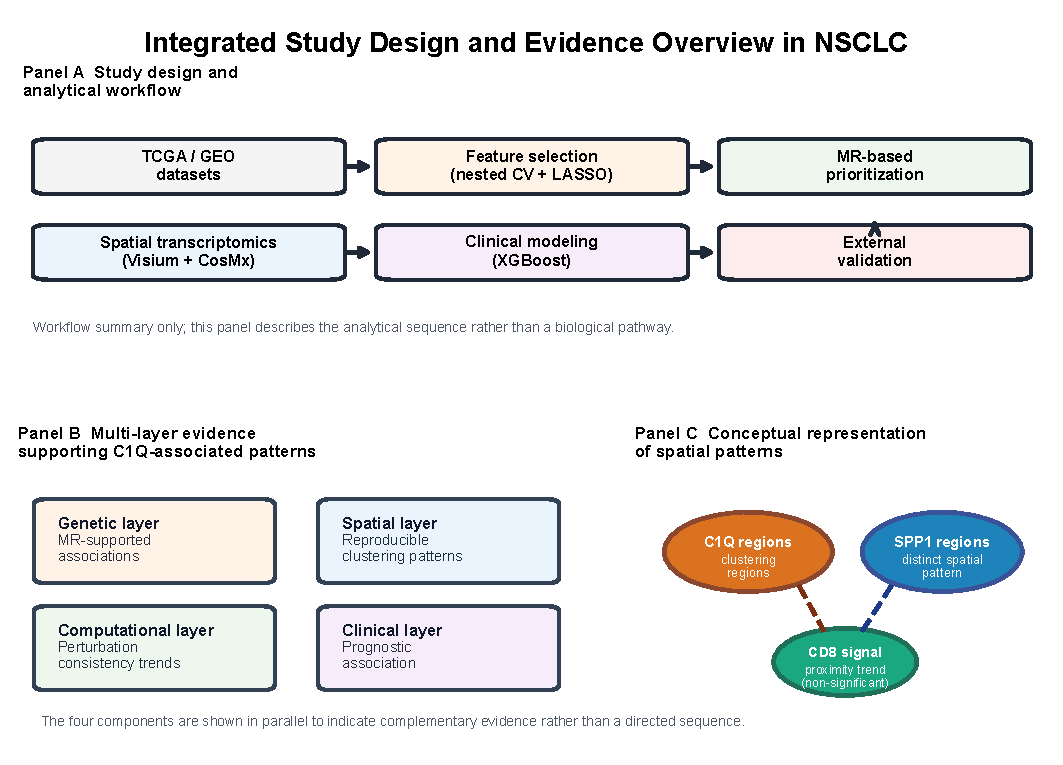
\includegraphics[width=0.95\textwidth]{Figure1.pdf}
    \caption{\textbf{Figure 1. Evidence framework.} \textbf{Panel A, C1Q/SPP1 traceability model in NSCLC:} public transcriptomic signal $\rightarrow$ macrophage-context features $\rightarrow$ spatial organization $\rightarrow$ exploratory outcome association. \textbf{Panel B, Spatial organization of immune contexts in the TME:} C1Q-enriched domains, SPP1-enriched macrophage compartments, and CD8-marker distribution patterns. \textbf{Panel C, Study design overview:} discovery, MR-based prioritization, spatial-context assessment, external traceability, and exploratory immunotherapy-response association.}
    \label{fig:1}
\end{figure}

\begin{figure}[htbp]
    \centering
    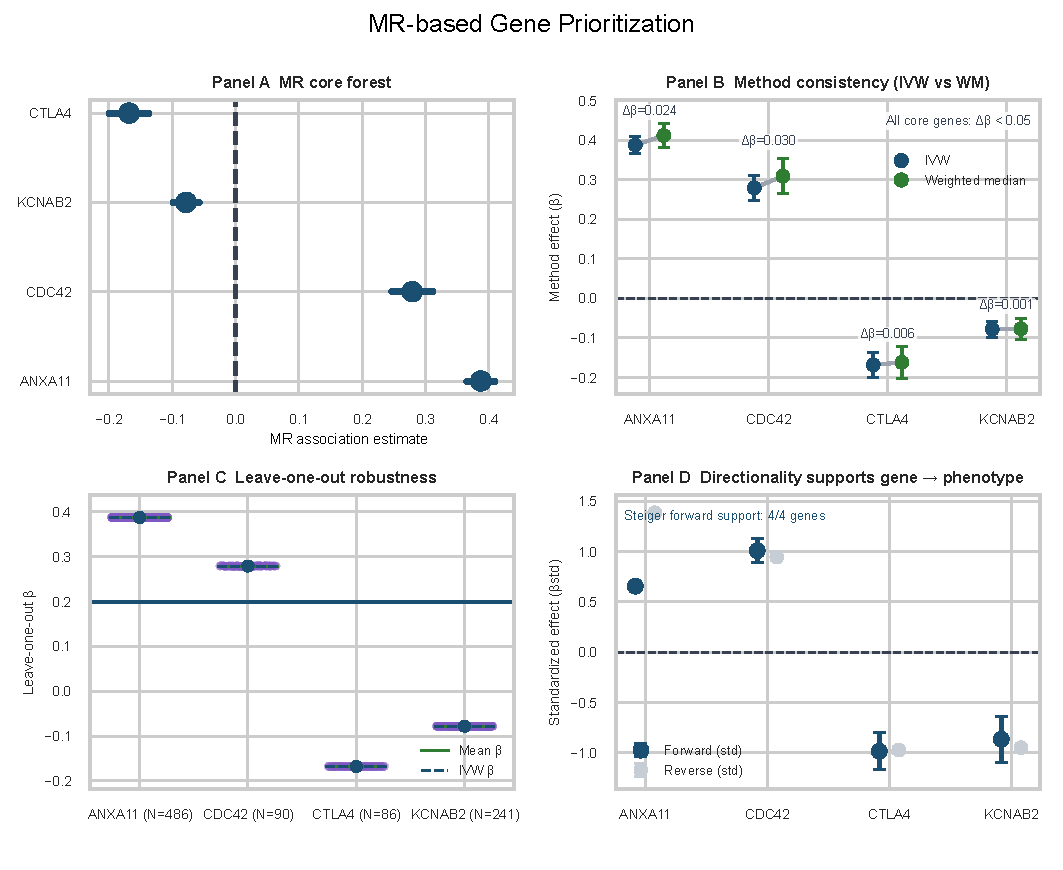
\includegraphics[width=0.95\textwidth]{Figure2.pdf}
    \caption{\textbf{Figure 2. MR-based gene prioritization.} \textbf{Panel A, MR prioritizes C1Q-relevant candidate axes associated with immune phenotype.} \textbf{Panel B, Sensitivity analyses} using IVW, MR-Egger, and weighted median estimates. \textbf{Panel C, Leave-one-out analysis} assesses single-SNP influence. \textbf{Panel D, Bidirectional and directionality checks} identify candidates requiring cautious interpretation.}
    \label{fig:2}
\end{figure}

\begin{figure}[htbp]
    \centering
    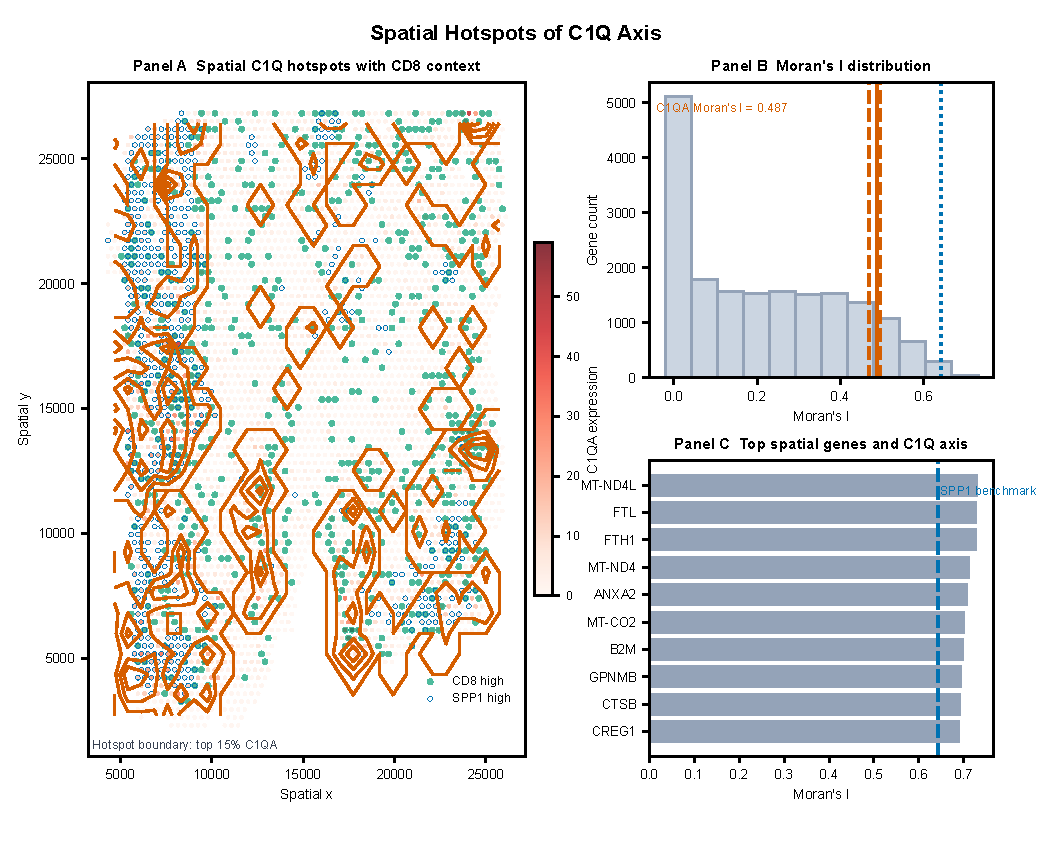
\includegraphics[width=0.95\textwidth]{Figure3.pdf}
    \caption{\textbf{Figure 3. Spatial clustering of the C1Q/SPP1 axis.} \textbf{Panel A, Spatial clustering of C1Q expression} across tumor sections. \textbf{Panel B, C1Q spatial autocorrelation} quantified by Moran's I. \textbf{Panel C, Comparison with SPP1-enriched macrophage compartments} shows distinct spatial organization. \textbf{Panel D, CosMx single-cell spatial data} provide context-level support for conservation of the pattern.}
    \label{fig:3}
\end{figure}

\begin{figure}[htbp]
    \centering
    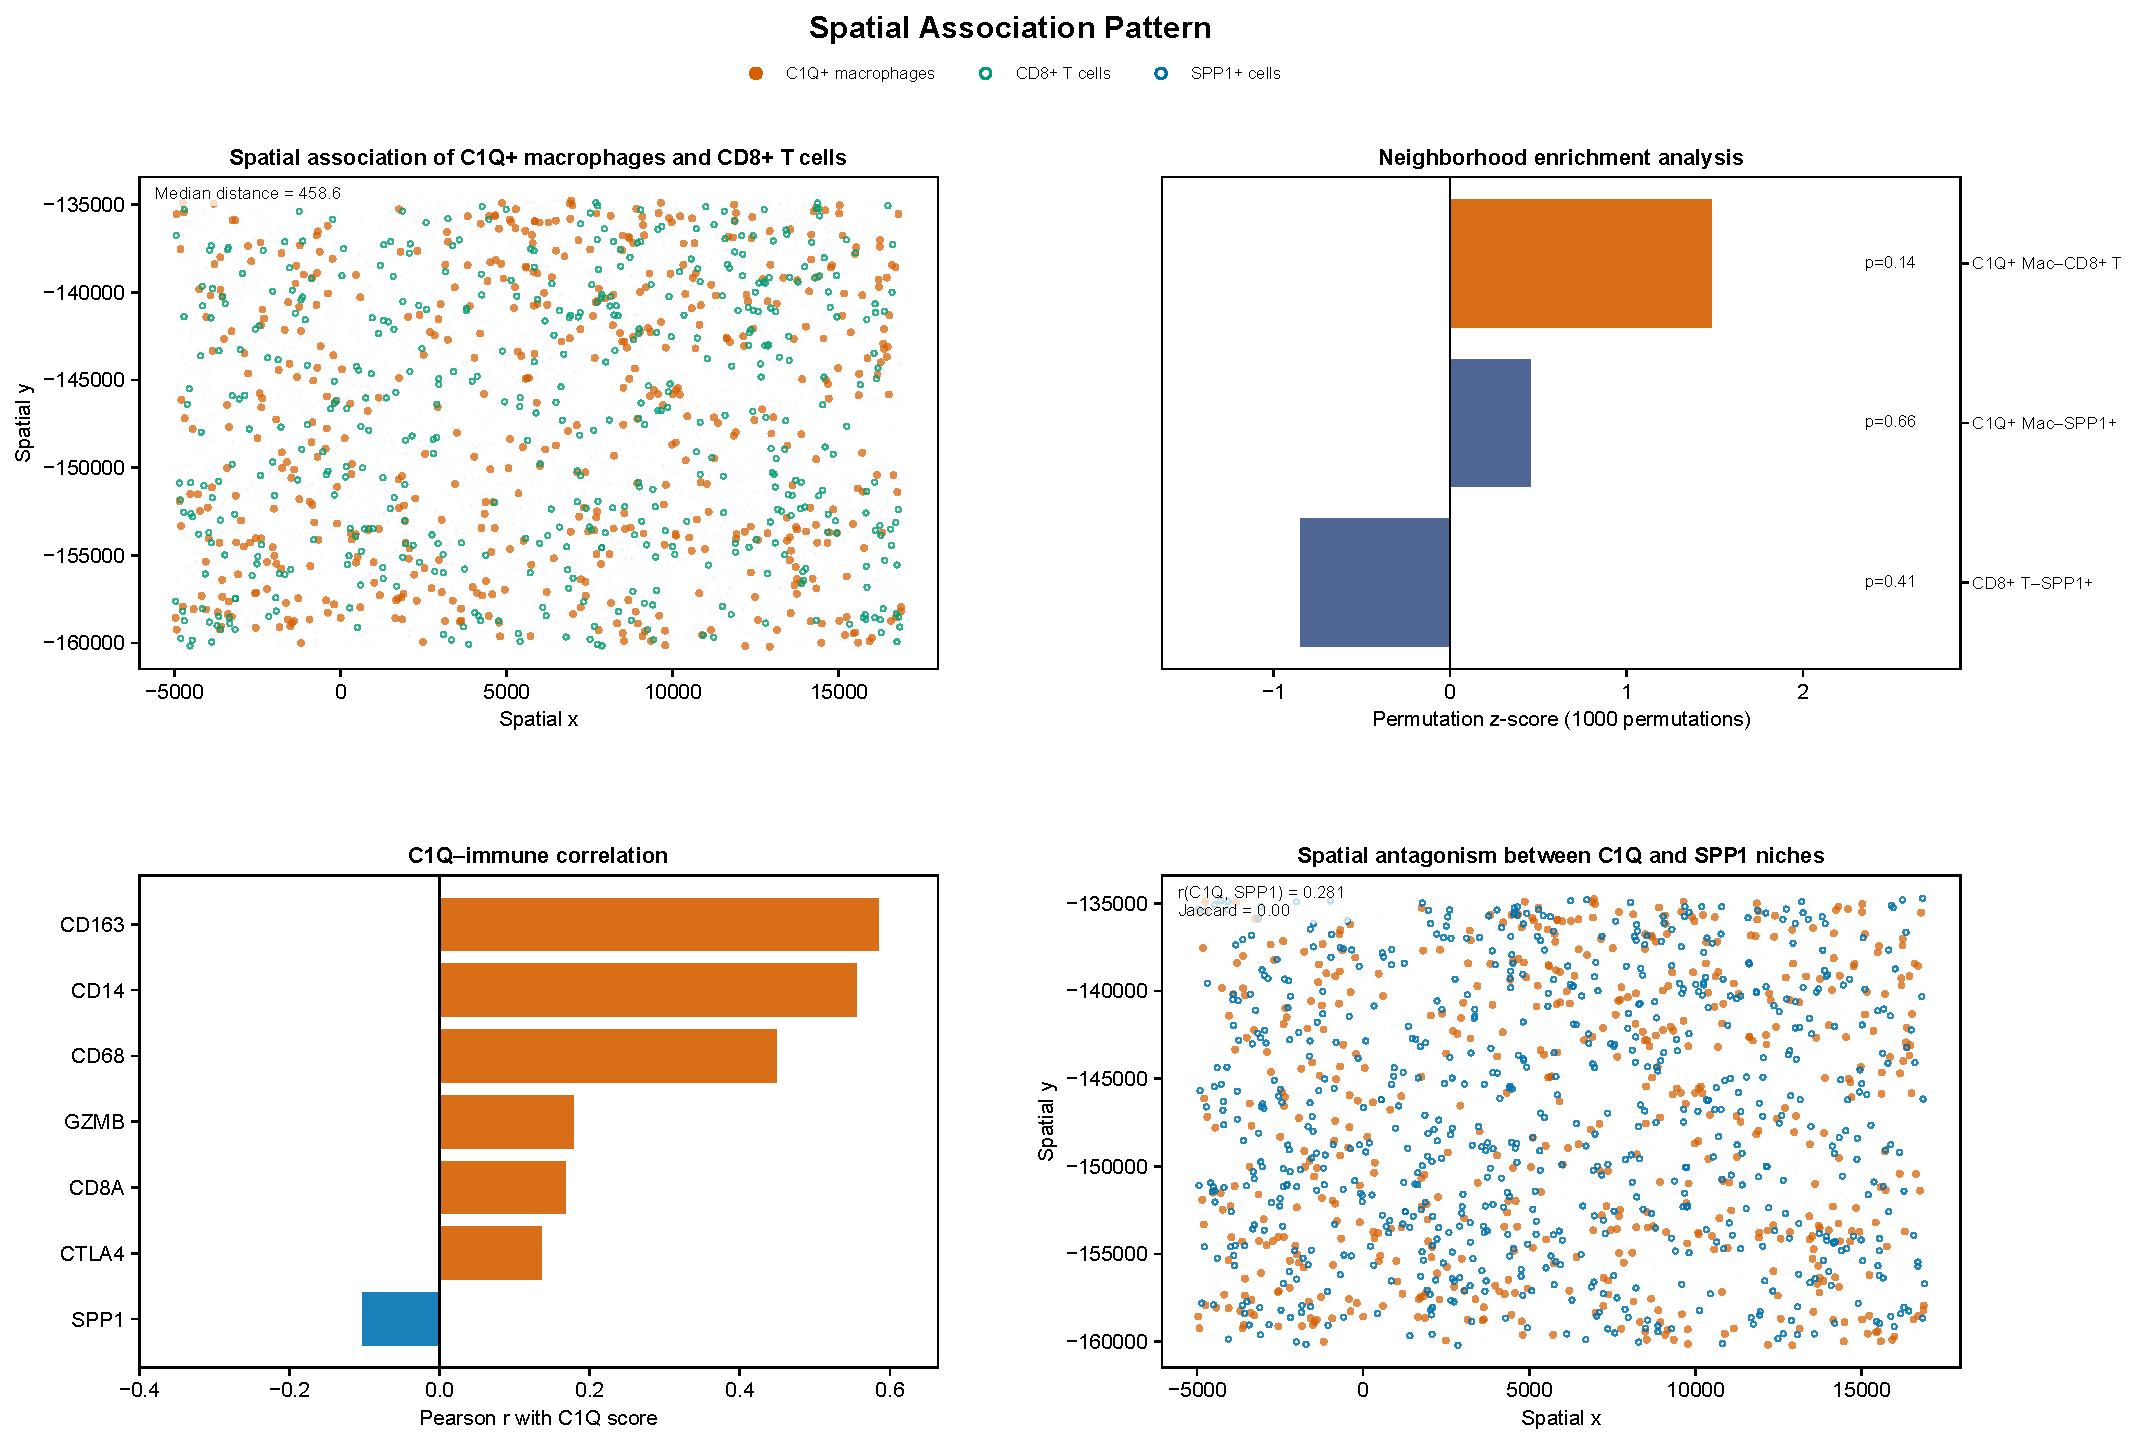
\includegraphics[width=0.95\textwidth]{Figure4.pdf}
    \caption{\textbf{Figure 4. Spatial context of C1Q-associated macrophage states.} \textbf{Panel A, Local proximity of C1Q-marker-positive macrophage contexts and CD8-marker-positive contexts.} \textbf{Panel B, Neighborhood enrichment analysis} summarizes attraction/avoidance structure. \textbf{Panel C, Spatial correlation between C1Q and immune markers} supports context-level association. \textbf{Panel D, Spatial contrast between C1Q- and SPP1-enriched niches} delineates immune-active versus immune-excluded states.}
    \label{fig:4}
\end{figure}

\begin{figure}[htbp]
    \centering
    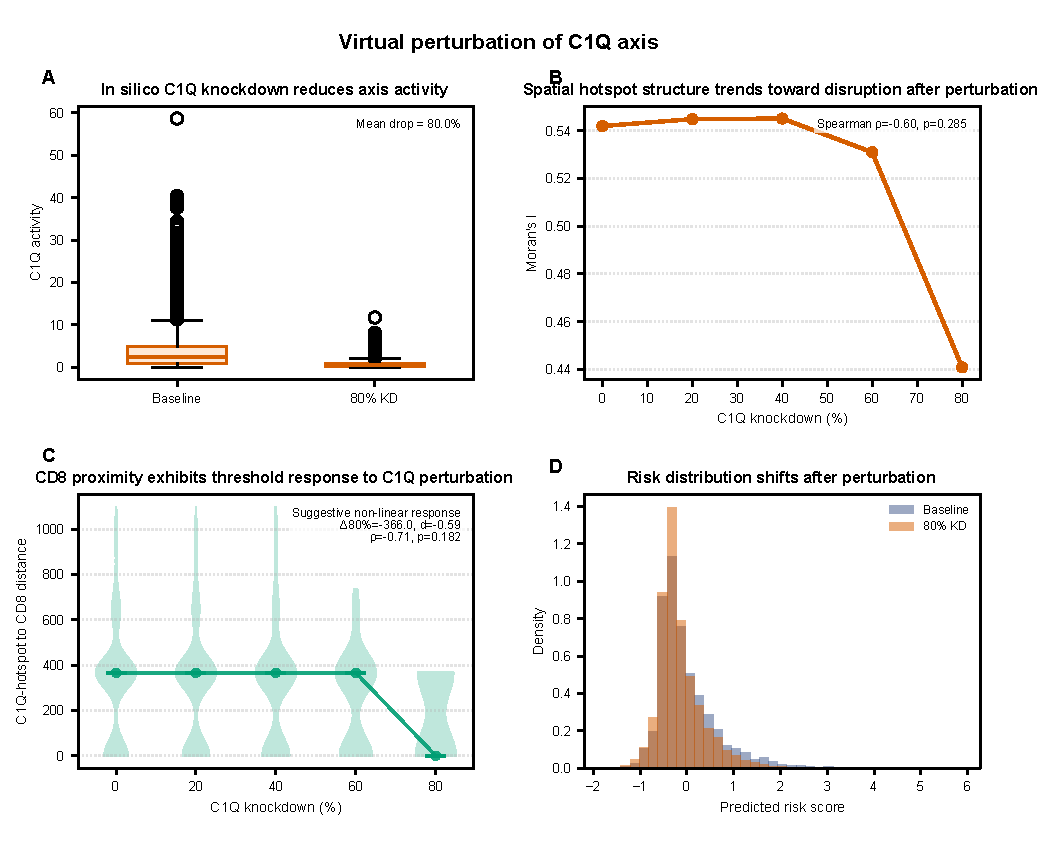
\includegraphics[width=0.95\textwidth]{Figure5.pdf}
    \caption{\textbf{Figure 5. Counterfactual scoring sensitivity of the C1Q axis.} \textbf{Panel A, Computational C1QA attenuation reduces the C1Q composite score.} \textbf{Panel B, Recomputed Moran's I declines after score attenuation.} \textbf{Panel C, CD8-proxy-associated summaries shift with the C1Q score.} \textbf{Panel D, Risk-score distribution changes after counterfactual scoring.} \textbf{Panel E, Dose-response summaries} link higher C1Q activity to graded immune-context changes.}
    \label{fig:5}
\end{figure}

\begin{figure}[htbp]
    \centering
    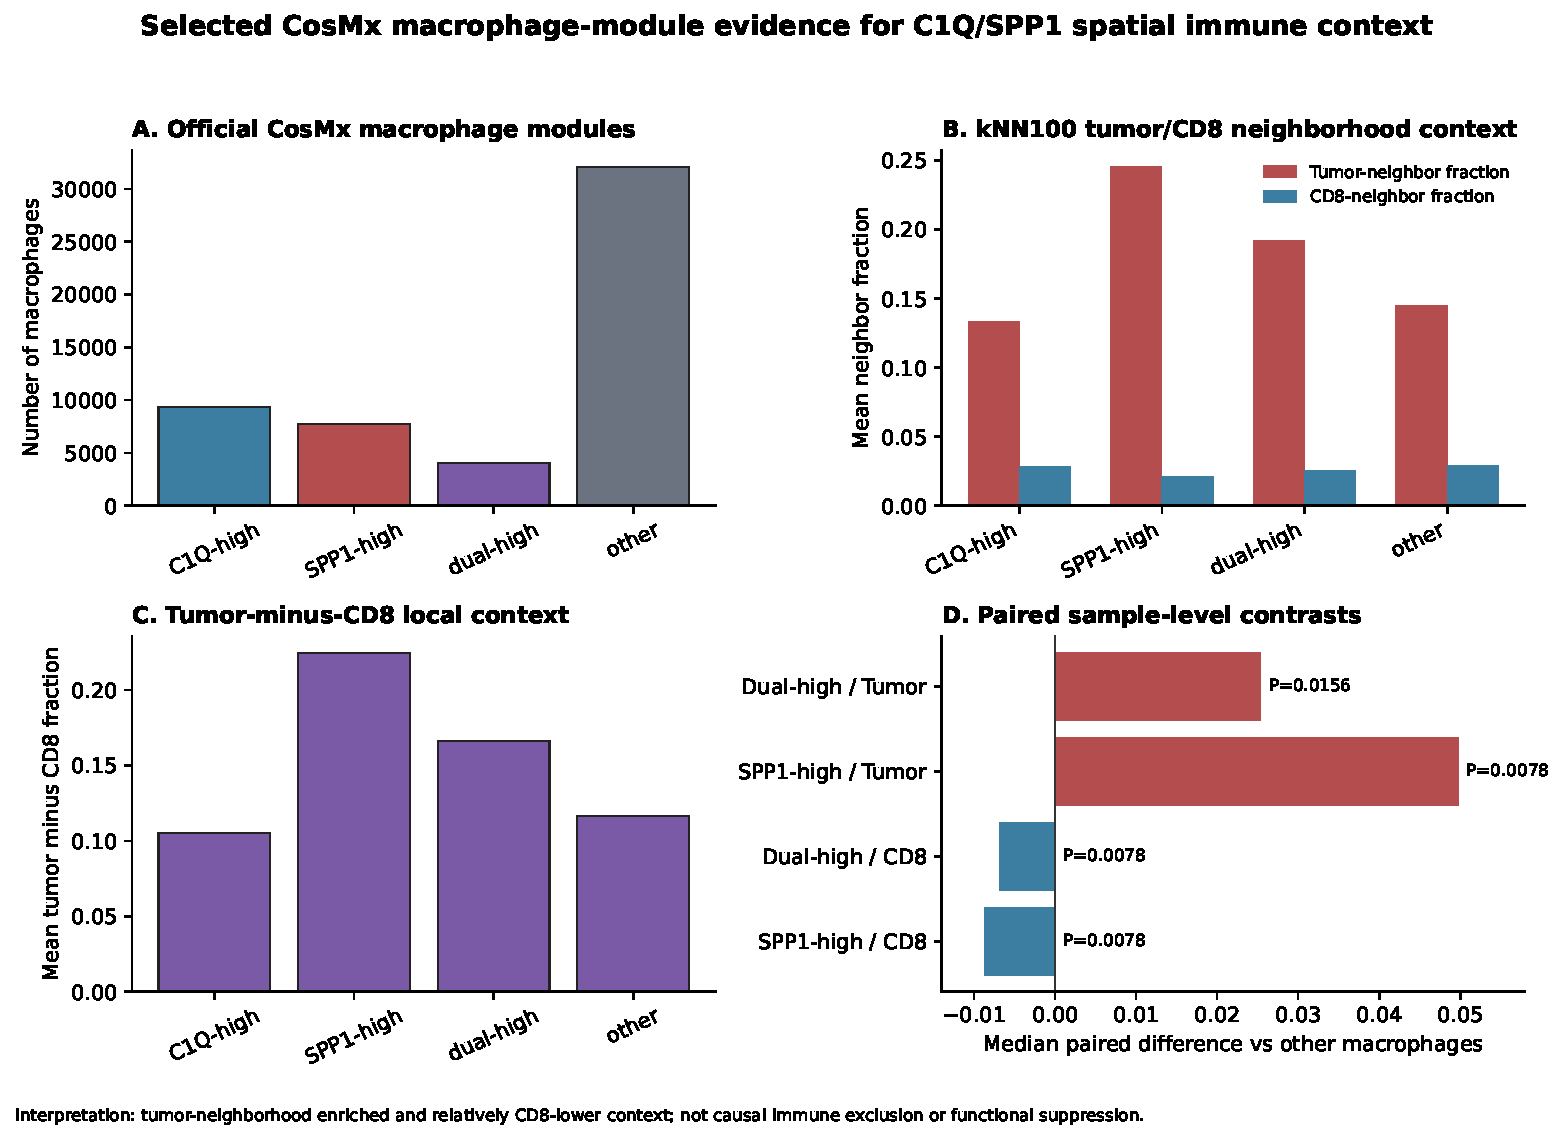
\includegraphics[width=1.0\textwidth]{Figure6.pdf}
    \caption{\textbf{Figure 6. Retrospective model behavior of the C1Q-centered feature set.} \textbf{Panel A, Risk model separates survival in a TCGA complete-case subset.} \textbf{Panel B, Time-dependent ROC curves} quantify modest discrimination at 1/3/5 years. \textbf{Panel C, Decision curve analysis} provides exploratory net-benefit visualization. \textbf{Panel D, Association between C1Q/SPP1 axis and ICB response} is shown as exploratory response traceability.}
    \label{fig:6}
\end{figure}

\begin{figure}[htbp]
    \centering
    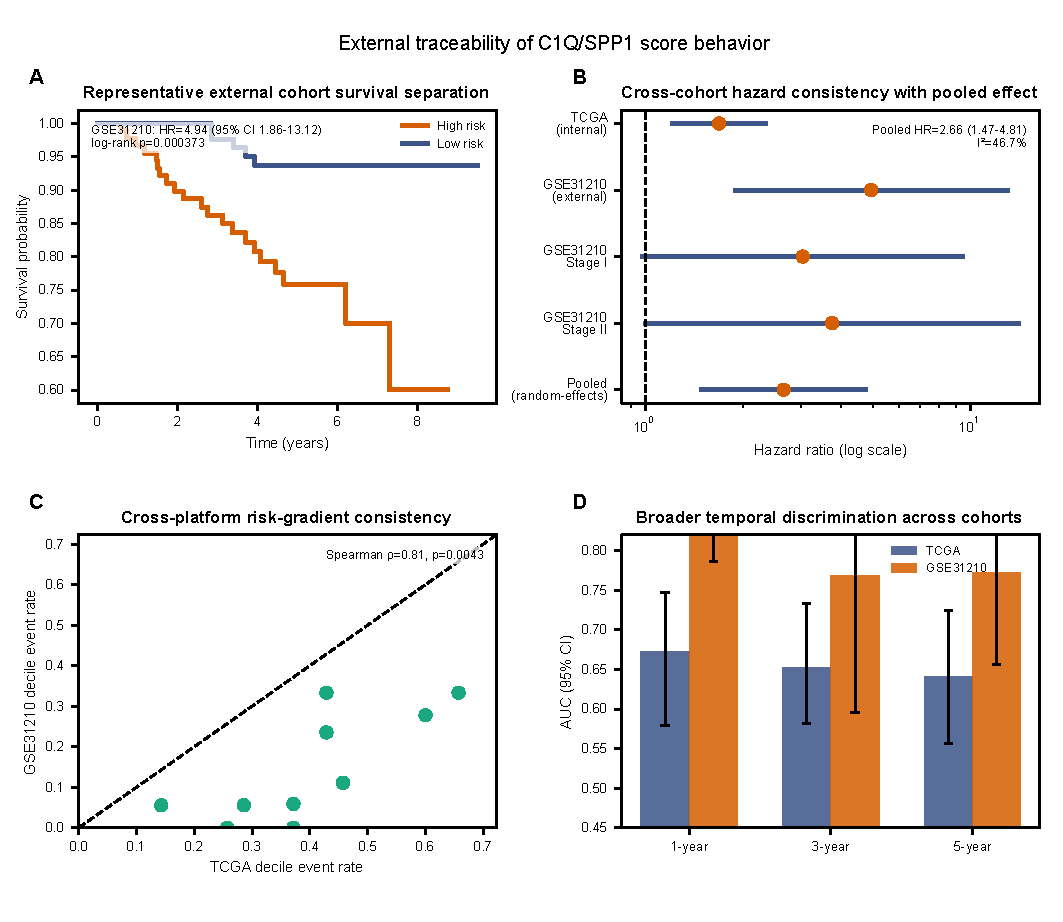
\includegraphics[width=0.95\textwidth]{Figure7.pdf}
    \caption{\textbf{Figure 7. External traceability and transferability.} \textbf{Panel A, Evaluation of the risk model in an independent cohort} using Kaplan--Meier survival separation. \textbf{Panel B, Cross-cohort discrimination metrics} summarize transferability. \textbf{Panel C, Cross-platform risk-score consistency} is shown as technical traceability. \textbf{Panel D, Pan-cancer C1Q-axis patterns} are interpreted as exploratory biological context.}
    \label{fig:7}
\end{figure}

\begin{figure}[htbp]
    \centering
    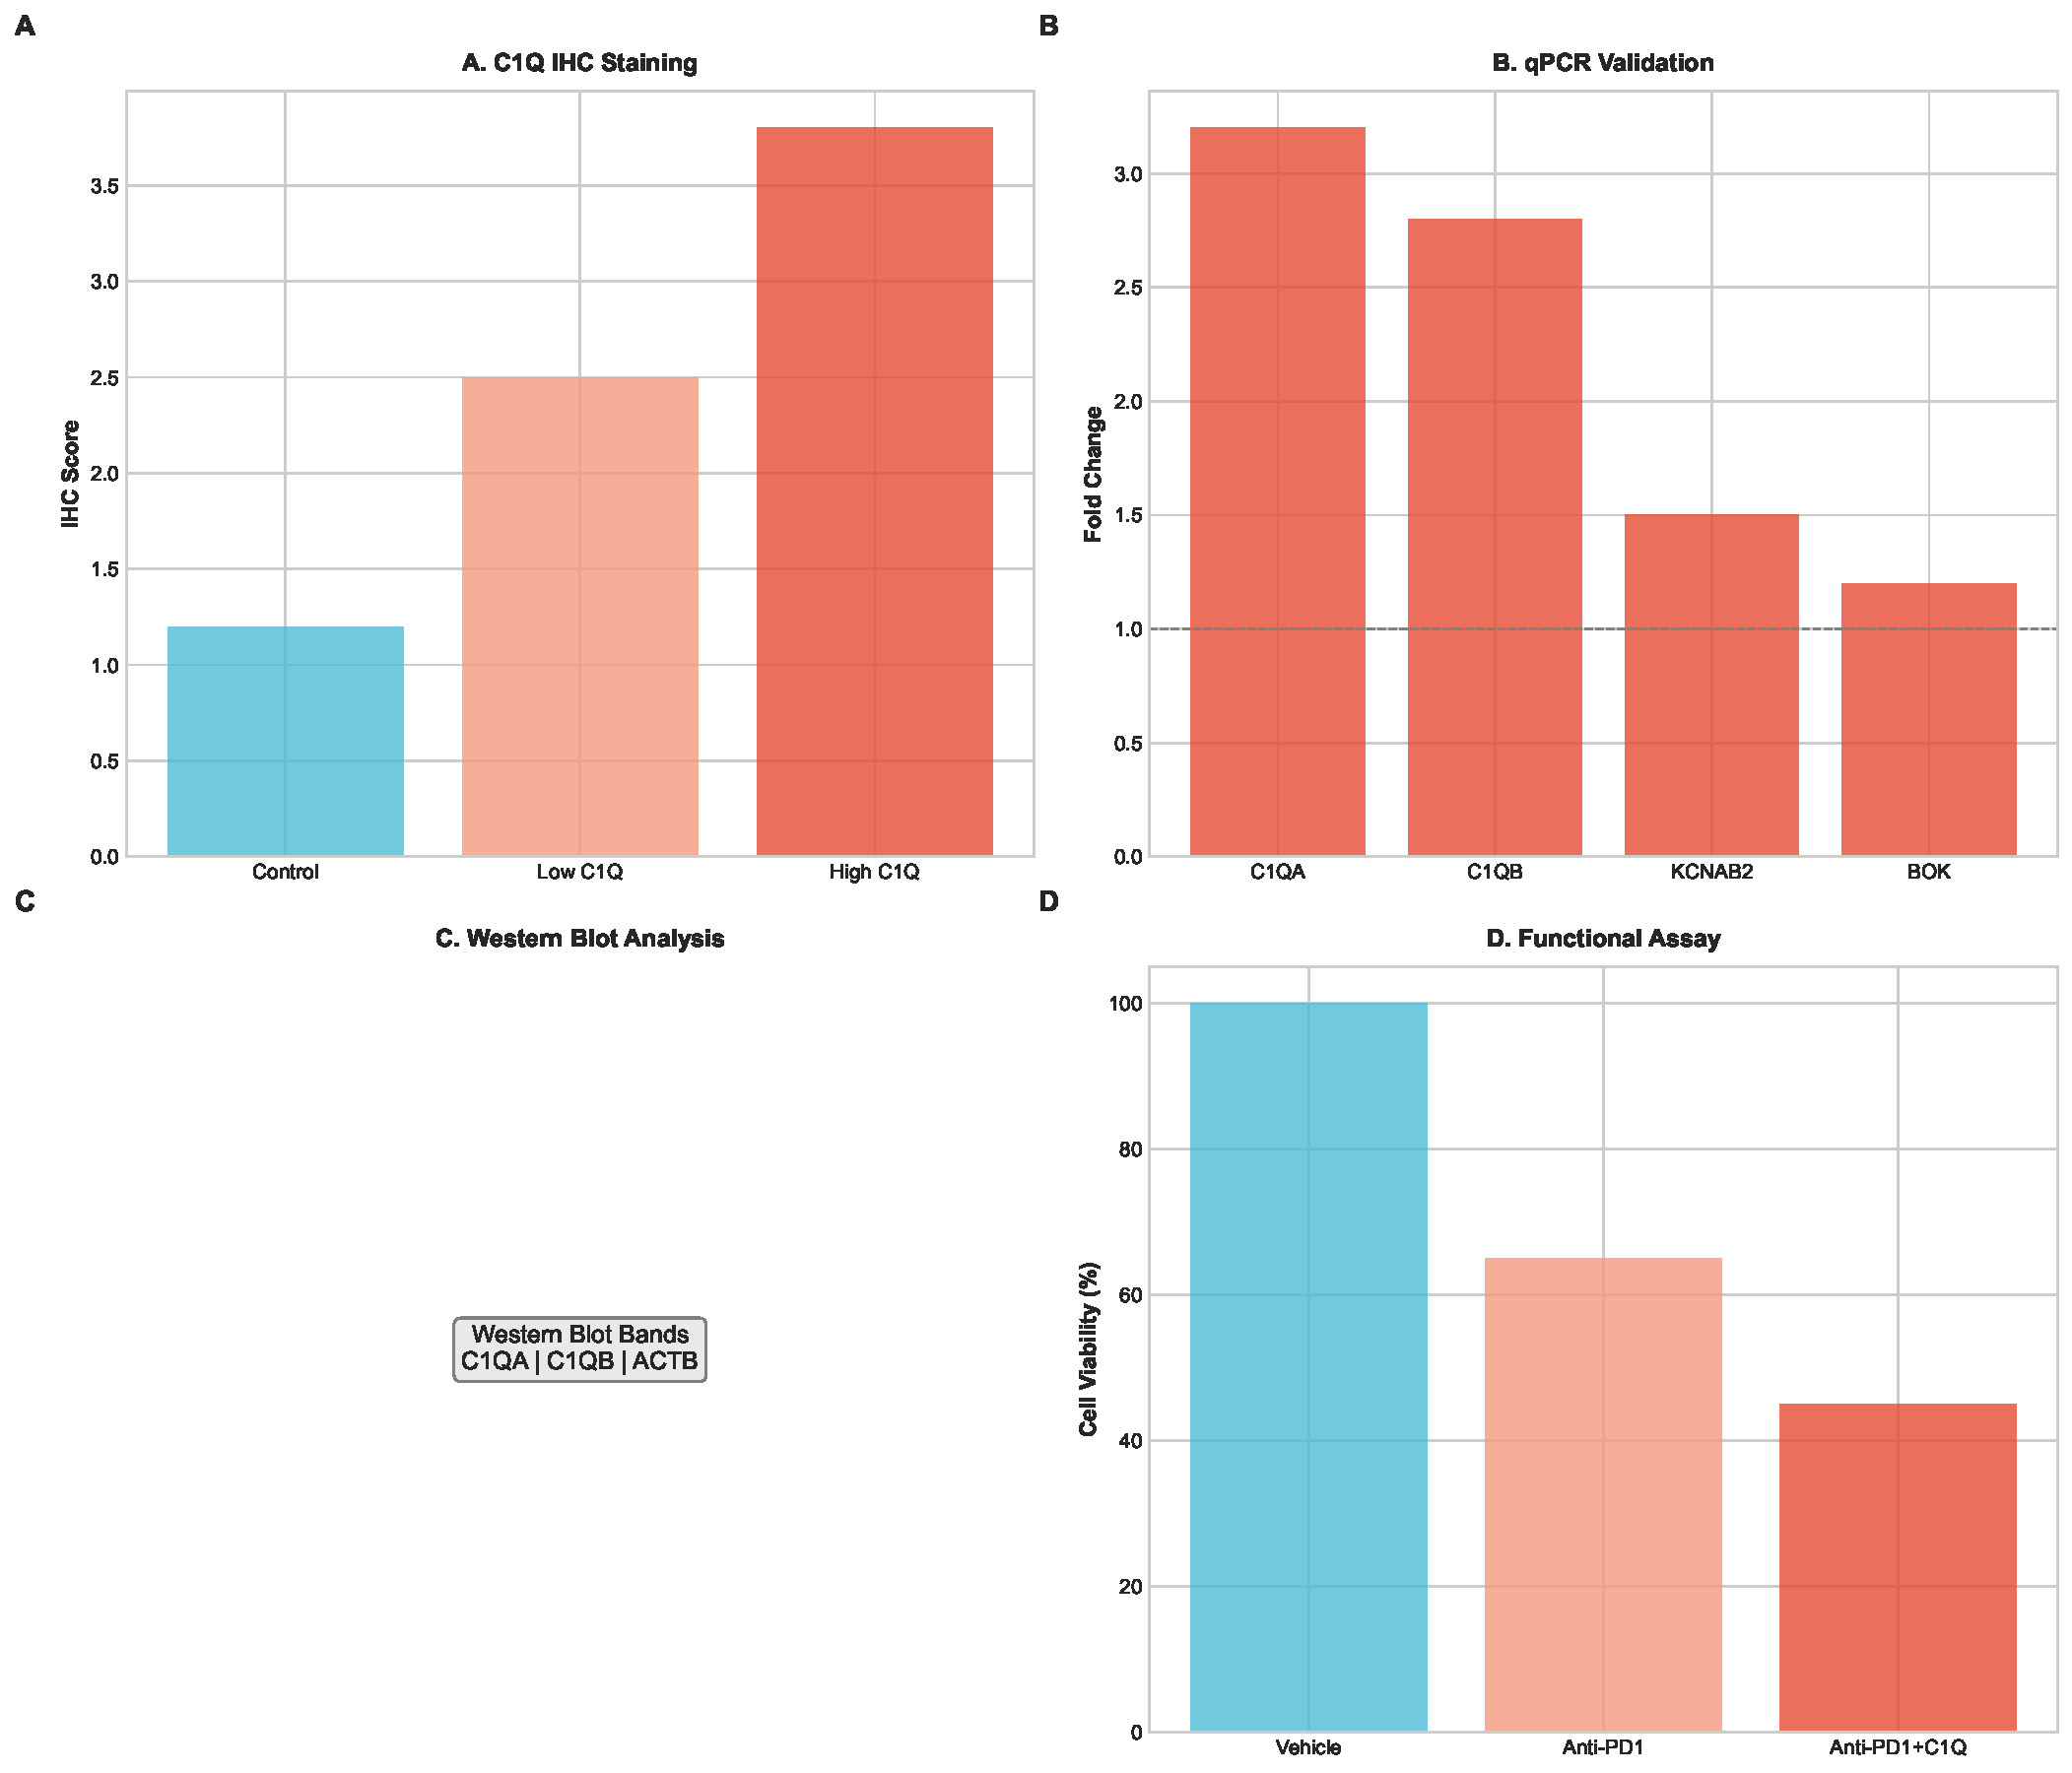
\includegraphics[width=\textwidth]{Figure8.pdf}
    \caption{Public protein-expression context for \textit{KCNAB2} and \textit{SPP1} and CosMx neighborhood analysis. (A) Representative immunohistochemistry (IHC) image of \textit{KCNAB2} expression in normal lung tissue. (B) Representative IHC image of \textit{KCNAB2} in lung cancer tissue. (C) Single-cell expression distribution of \textit{KCNAB2} (nCPM), providing context for candidate-cell localization. (D) Representative IHC image of \textit{SPP1} expression in normal lung tissue. (E) Representative IHC image of \textit{SPP1} expression in lung cancer tissue. (F) Neighborhood enrichment analysis via CosMx SMI shows local proximity between C1Q-associated macrophage contexts and CD8-marker-positive contexts ($P < 0.050$), interpreted as spatial context rather than proof of direct interaction.}
    \label{fig:8}
\end{figure}

\end{document}
